\section{Задание 1. Линейные фильтры}
Зададимся числами $a$, $t_1$, $t_2$ такими, что $t_1 < t_2$, и построим функцию
\[
g(t) = 
\begin{cases}
a, & t \in [t_1, t_2], \\
0, & t \notin [t_1, t_2];
\end{cases}
\]
и её зашумлённую версию
\[
u(t) = g(t) + b\xi(t) + c \sin(dt),
\]
где $\xi(t) \sim \mathcal{U} [-1, 1]$ - равномерное распределение, представляющее белый шум, а значения $b$, $c$, $d$ - параметры возмущения.

\subsection{Фильтр первого порядка}
Применим $c=0$. Зададим постоянную времени $T>0$ и пропустим сигнал $u(t)$ через линейный фильтр первого порядка
$$
W_1(p)=\frac{1}{Tp+1}.
$$
Построим сравнительные графики исходного и фильтрованого сигналов, графики модулей их Фурье-образов, а так же АЧХ фильтра. Исследуем влияние постоянной времени $T$ и значение параметра $a$ на эффективность фильтрации.\newline
Графики сигналов представлены на рис. \ref{fig:1}-\ref{fig:3}, графики Фурье-образов на рис. \ref{fig:4}-\ref{fig:6}, АЧХ фильтра на рис. \ref{fig:7}.

\textbf{Анализ}
\newline
Из графиков видим, что параметр $T=\frac{1}{\omega_c}$ влияет на сглаживание и запаздывание сигнала. При увеличении $T$ остаётся меньше шумов, но при этом увеличивается запаздывание сигнала и он теряет свою форму. По сути, $T$ - это время отклика, насколько быстро фильтр реагирует на изменение сигнала. Поэтому при увеличении $T$ увеличивается запаздывание, но фильтр накапливает больше информацции о сигнале и фильтрация шумов получается более эффективной.
\newline
Наиболее оптимальным в нашем варианте является  $T\approx0.1$ при $a=2$ и $T=0.025$ при остальных $a$, при таких комбинациях остаётся мало шума, и форма сигнала близка к оригиналу.
\newline
Параметр $a$ определяет амплитуду сигнала $g(t)$. При большем $a$ зашумленный сигнал эффективнее фильтруется, так как мы рассматриваем фиксированные параметры генерации шума, и при большей амплитуде исходного сигнала, отношение сигнал/шум увеличивается, делая шум менее заметным относительно полезного сигнала.
\newline
Посмотрим на графики Фурье-образа: подавление верхних частот происходит постепенно - чем больше частота, тем сильнее уменьшается её амплитуда. Для более точного объяснение обратимся к графикам АЧХ, на которых видим, что в данном фильтре подавление частот происходит на всём спектре (нет усиления выбранных частот), и при увеличении $T$ фильтр начинает подавлять высокочастотные помехи быстрее, фильтр становится более "жёстким".
\newline
На графиках \ref{fig:8} - \ref{fig:13} представлена проверка теоремы о свёртке для временной и частотной области. Эксперимент подтвердил теоретические ожидания.


\begin{figure}[H]
    \centering
    
\includegraphics[width=1.0\linewidth]{fig/plots/Figure 1.png}
    \caption{Сигнал}
    \label{fig:1}
\end{figure}\begin{figure}[H]
    \centering
    
\includegraphics[width=1.0\linewidth]{fig/plots/Figure 2.png}
    \caption{Сигнал}
    \label{fig:2}
\end{figure}\begin{figure}[H]
    \centering
    
\includegraphics[width=1.0\linewidth]{fig/plots/Figure 3.png}
    \caption{Сигнал}
    \label{fig:3}
\end{figure}

\begin{figure}[H]
    \centering
    
\includegraphics[width=1.0\linewidth]{fig/plots/Figure 4.png}
    \caption{Фурье-образ}
    \label{fig:4}
\end{figure}\begin{figure}[H]
    \centering
    
\includegraphics[width=1.0\linewidth]{fig/plots/Figure 5.png}
    \caption{Фурье-образ}
    \label{fig:5}
\end{figure}\begin{figure}[H]
    \centering
    
\includegraphics[width=1.0\linewidth]{fig/plots/Figure 6.png}
    \caption{Фурье-образ}
    \label{fig:6}
\end{figure}

\begin{figure}[H]
    \centering
    
\includegraphics[width=1.0\linewidth]{fig/plots/Figure 7.png}
    \caption{АЧХ}
    \label{fig:7}
\end{figure}

\begin{figure}[H]
    \centering
    
\includegraphics[width=1.0\linewidth]{fig/plots/Figure 8.png}
    \caption{Временная область}
    \label{fig:8}
\end{figure}\begin{figure}[H]
    \centering
    
\includegraphics[width=1.0\linewidth]{fig/plots/Figure 9.png}
    \caption{Временная область}
    \label{fig:9}
\end{figure}\begin{figure}[H]
    \centering
    
\includegraphics[width=1.0\linewidth]{fig/plots/Figure 10.png}
    \caption{Временная область}
    \label{fig:10}
\end{figure}

\begin{figure}[H]
    \centering
    
\includegraphics[width=1.0\linewidth]{fig/plots/Figure 11.png}
    \caption{Частотная область}
    \label{fig:11}
\end{figure}\begin{figure}[H]
    \centering
    
\includegraphics[width=1.0\linewidth]{fig/plots/Figure 12.png}
    \caption{Частотная область}
    \label{fig:12}
\end{figure}\begin{figure}[H]
    \centering
    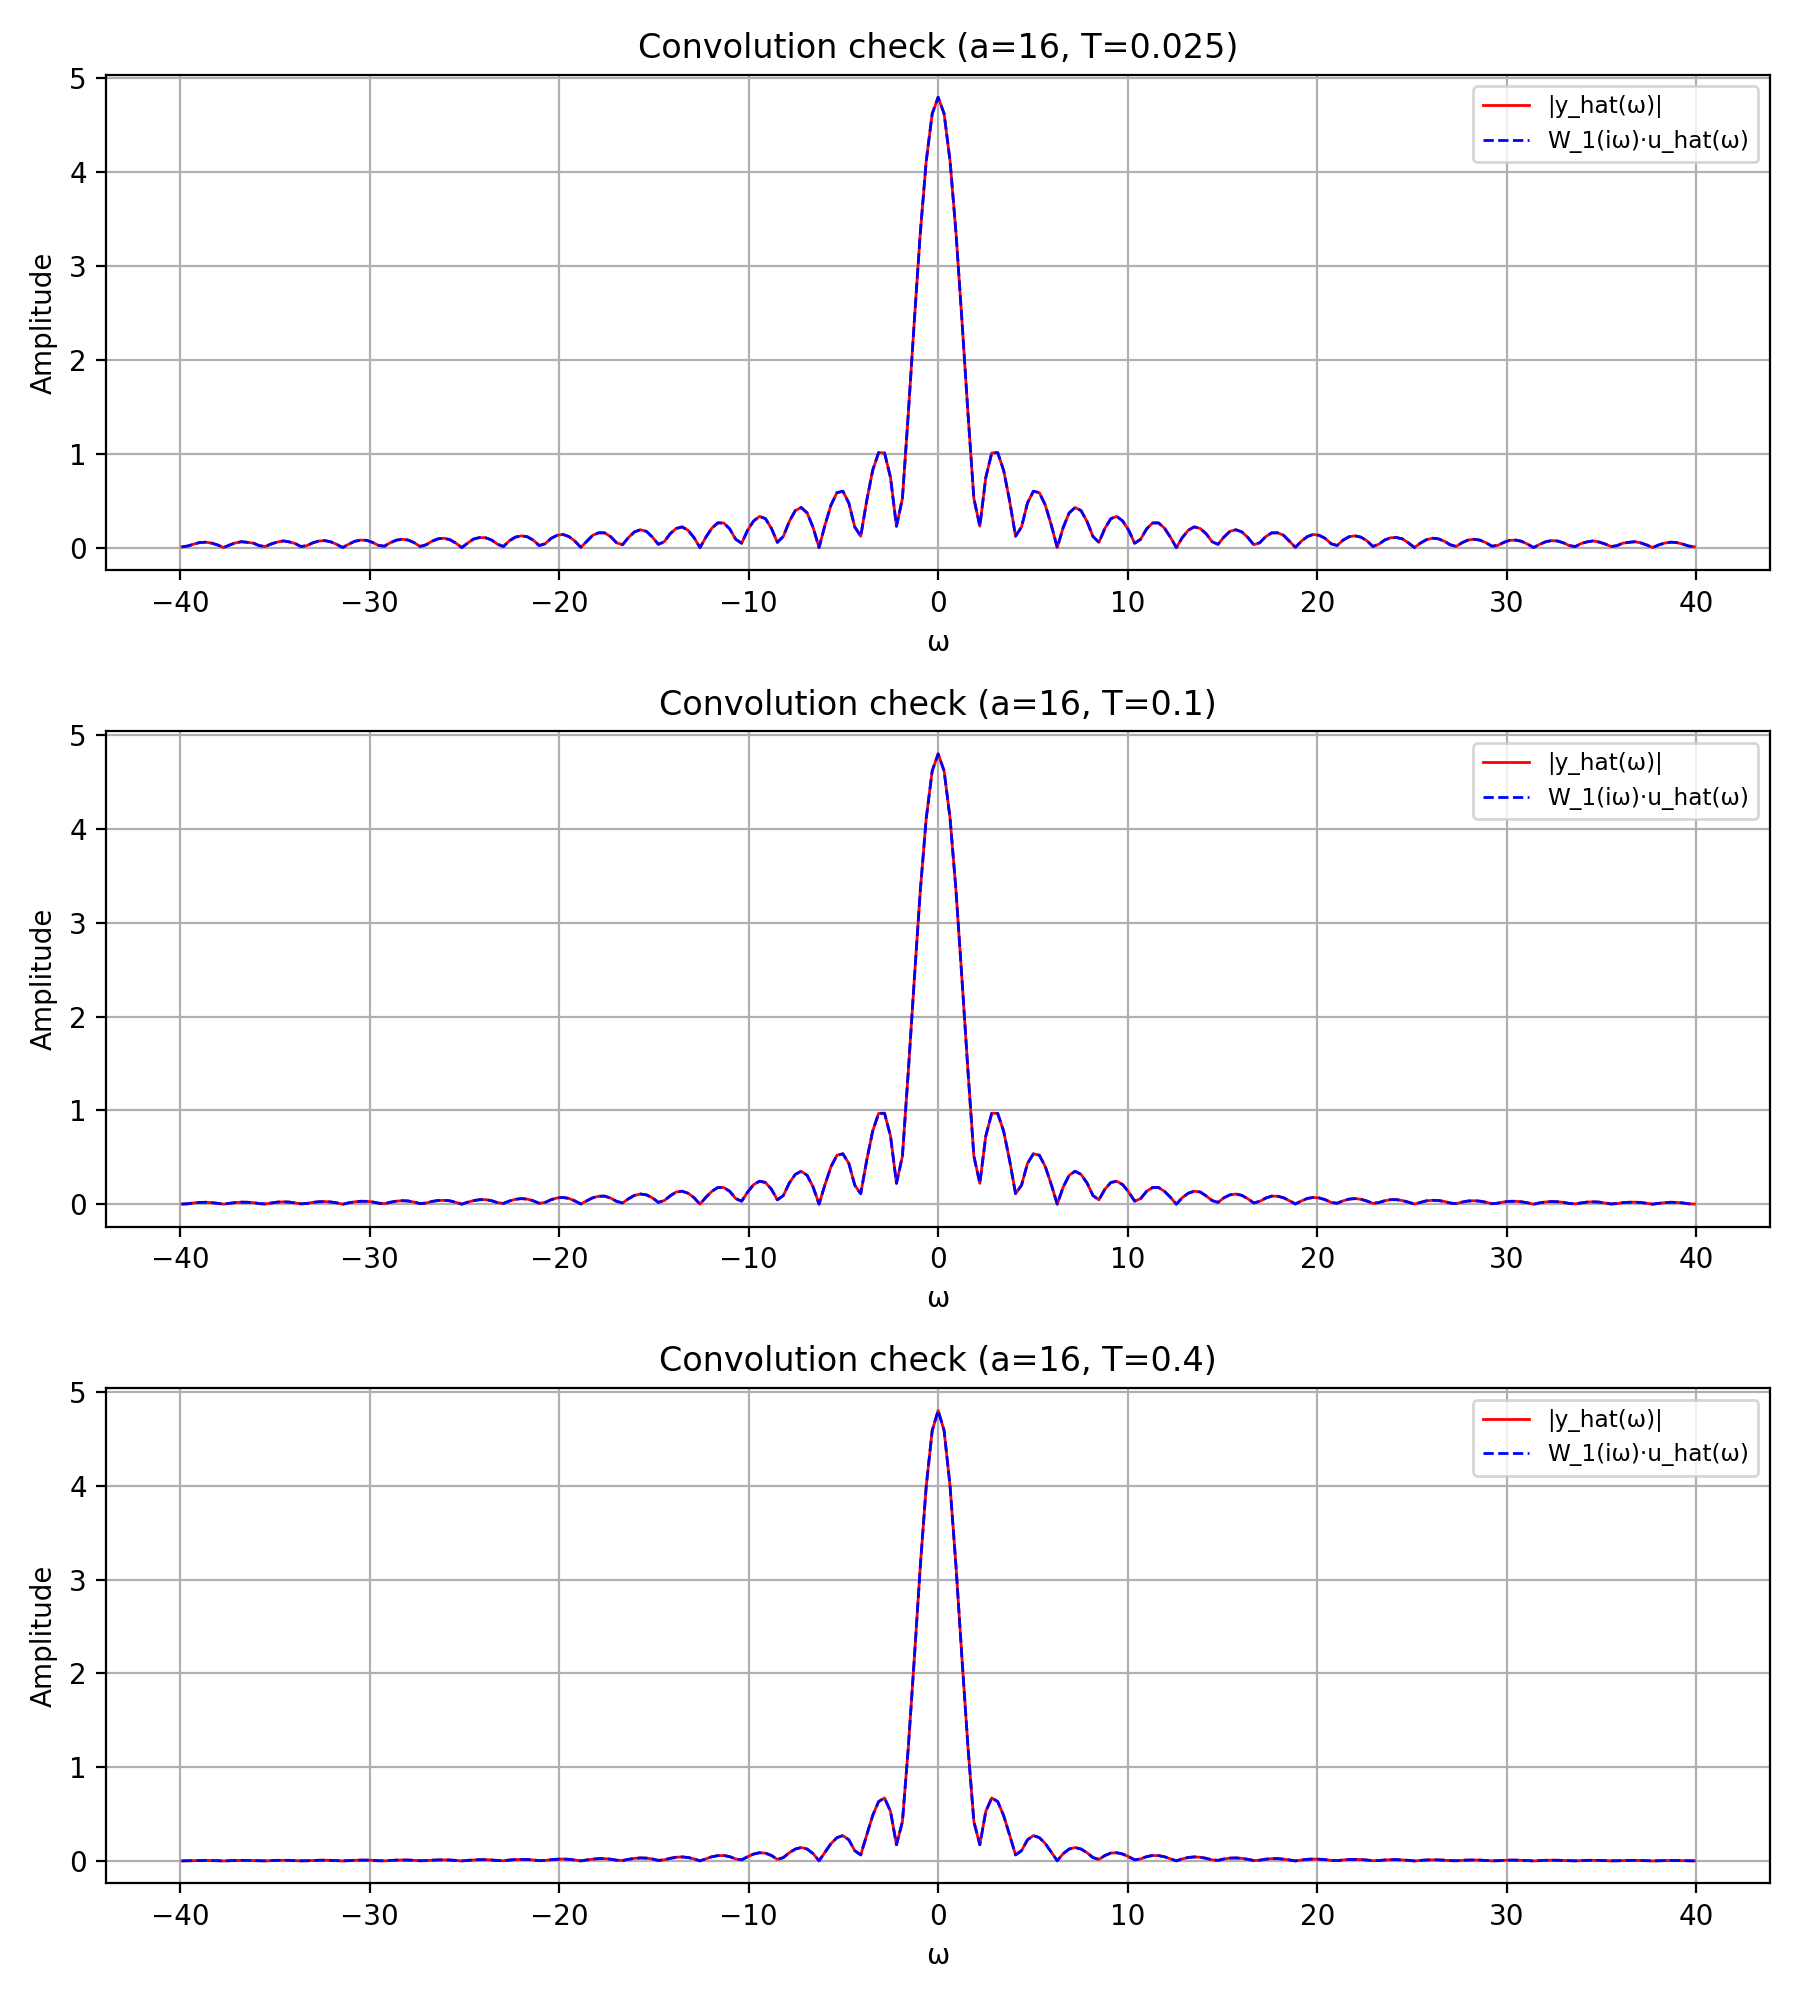
\includegraphics[width=1.0\linewidth]{fig/plots/Figure 13.png}
    \caption{Частотная область}
    \label{fig:13}
\end{figure}


\textbf{Выводы}
\newline
Полученные в результате исследования данные согласуются с теоретическим представлением о динамическом фильтре низких частот.
\newline
Параметр $T$ тем меньше можно выбирать, чем больше $a$, а при более близком $a$ к амплитуде шума $b$ (в нашем случае, $b=0.5$), параметр $T$ приходится увеличивать, иначе в отфильтрованном сигнале сохраняется много помех. Теорема о свёртке выполняется.

\subsection{Режекторный полосовой фильтр}
Примем $b = 0$. Рассмотрим линейный фильтр вида
$$
W_2(p) = \frac{p^2 + a_1 p + a_2}{p^2 + b_1 p + b_2}.
$$
Выберем значения параметров $a_1, a_2, b_1, b_2 \in \mathbb{R}$ исходя из условий:
\begin{itemize}
    \item Фильтр должен быть устойчивым (корни полинома знаменателя $p_1, p_2$ должны иметь строго отрицательную вещественную часть).
    \item Для нижних частот ($\omega \to 0$) и верхних частот ($\omega \to \infty$) АЧХ фильтра должна быть равна 1.
    \item Для некоторой частоты $\omega_0$ АЧХ фильтра должна быть равна 0.
\end{itemize}
Построим сравнительные графики исходного и фильтрованного сигналов, графики модулей их Фурье-образов, а также АЧХ фильтра. Исследуем влияние параметра $c$ и $d$ на эффективность фильтрации.\newline
Обеспечим выполнимость условий:
\begin{itemize}
    \item Корни полинома $p^2 + b_1 p + b_2$ гарантированно будут иметь отрицательную вещественную часть при $\text{Re}(\frac{-b_1\pm\sqrt{b_1^2-4a_2}}{2})<0$
    
    \item При $\omega \to 0$: $W(i\omega) = \frac{a_2}{b_2} = 1 \Rightarrow a_2 = b_2$
    
    \item При $\omega \to \infty$: $W(i\omega) = \lim_{\omega\to\infty} \frac{(i\omega)^2 + a_1(i\omega) + a_2}{(i\omega)^2 + b_1(i\omega) + b_2} = \frac{-1 + \frac{a_1}{i\omega} + \frac{a_2}{\omega^2}}{-1 + \frac{b_1}{i\omega} + \frac{b_2}{\omega^2}} \to 1$, что выполняется автоматически при $a_2 = b_2$
    
    \item Для частоты $\omega_0$ АЧХ равна нулю: $|W(i\omega_0)| = 0 \Rightarrow (i\omega_0)^2 + a_1(i\omega_0) + a_2 = 0$. Отсюда получаем систему:
  $$\begin{cases}
        -\omega_0^2 + a_2 &= 0\\
        a_1 \omega_0 &= 0
    \end{cases}$$
    Так как $\omega_0 \neq 0$, то $a_1 = 0$ и $a_2 = \omega_0^2$.
\end{itemize}

Рассмотрим следующие параметры:
$$
a=1,\
c = \{0.1, 0.5\},\
d = \{20, 25, 30\},\
a_1 = 0,\
a_2 = b_2 = 625,\
b_1 = \{5, 20, 70, 200\} 
$$



Графики сигналов представлены на рис. \ref{fig:14} - \ref{fig:21}, графики Фурье-образов на рис. \ref{fig:22} - \ref{fig:29}, АЧХ фильтра на рис. \ref{fig:30}.\newline
\textbf{Анализ}
\newline
Параметр $c$ влияет на амплитуду гармоники, $d$ - на её частоту. $b_1$ - на ширину полосы $\Delta\omega$ при $|W(i\omega)|=\frac{1}{\sqrt{2}}$, покажем  это:
\newline
Рассмотрим передаточную функцию режекторного фильтра второго порядка:

$$
W_2(p) = \frac{p^2 + \omega_0^2}{p^2 + b_1 p + \omega_0^2}
$$
где $\omega_0$ - центральная частота подавления.

Учитывая определение АЧХ фильтра:

$$
|W(i\omega)| = \frac{|\omega_0^2 - \omega^2|}{\sqrt{(\omega_0^2 - \omega^2)^2 + (b_1 \omega)^2}}
$$

Получаем:

$$
\frac{(\omega_0^2 - \omega^2)^2}{(\omega_0^2 - \omega^2)^2 + (b_1 \omega)^2} = \frac{1}{2};\quad 
(\omega_0^2 - \omega^2)^2 = (b_1 \omega)^2;\quad
\omega_0^2 - \omega^2 = \pm b_1 \omega
$$$$
\omega_\pm = \frac{\pm b_1 + \sqrt{b_1^2 + 4\omega_0^2}}{2}\quad\text{(для $\omega>0$)}
$$

Разность граничных частот дает искомую ширину полосы:
$$
\Delta\omega = \omega_+ - \omega_- = b_1
$$
Данный фильтр лучше всего подавляет гармонику в том случае, когда её частота совпадает с $\omega_0$, что согласуется с теоретическими ожиданиями: на этой частоте АЧХ фильтра зануляется. Чем большее разница $|d-\omega_0|$, тем меньше гармоника подавляется. Причем из графика АЧХ видно, что при удалении $d$ от $\omega_0$ подавление происходит сильнее, если $d$ находится в области более высоких частот, чем $\omega_0$. В то же время, при увеличении $b_1$ область, в которой гармоника подавляется эффективно, увеличивается, и поэтому возрастает разница $|d-\omega_0|$, при которой всё ещё получится хорошо приблизиться к исходному сигналу после фильтрации. Однако, при увеличении $b_1$ растёт и запаздываение сигнала (аналогичное явление мы наблюдали в предыдущем пункте), поэтому увеличивать $b_1$ очень сильно тоже не получится. На графике АЧХ это довольно наглядно, чем шире окно $\Delta\omega= b_1$, тем у большего количества частот "режется" амплитуда.
\newline
При увеличении амплитды гармоники $c$ сглаживание происходит немного хуже, но при совпадении $d=\omega_0$ данный параметр почти не влияет.
\newline
Так же заметен эффект Гибса, который усиливается при увеличении $b_1$.
\newline
На графиках \ref{fig:31} - \ref{fig:46} представлена проверка теоремы о свёртке для временной и частотной области. Эксперимент подтвердил теоретические ожидания. Так же мы можем заметить, что для данного сигнала графики в некоторой степени расходятся в области около нуля (если точнее, в начальный момент времени и некоторое малое время спустя него), что вызванно особенностью того, как считается функция \texttt{lsim} (начальными условиями для неё). В следующем задании мы явно зададим начальные условия для того, чтобы скорректировать данную погрешность и увидеть, как с ней можно бороться.


\textbf{Выводы}
\newline
Полученные в результате исследования данные согласуются с теоретическим представлением о динамическом режекторном полосовом фильтре.
\newline
Лучшая фильтрация происходит при $d=\omega_0$ для любого $b_1$ - по сути, фильтровать именно эту частоту и есть задача данного фильтра. При увеличении $b_1$ до некоторых значений мы можем эффективно подавлять б\`ольшую полосу частот. При слишком сильном увеличении данного параметра фильтрованный сигнал начинает сильно запаздывать. Параметр $c$ также оказывает влияение на качество фильтрации.

\begin{figure}[H]
    \centering
    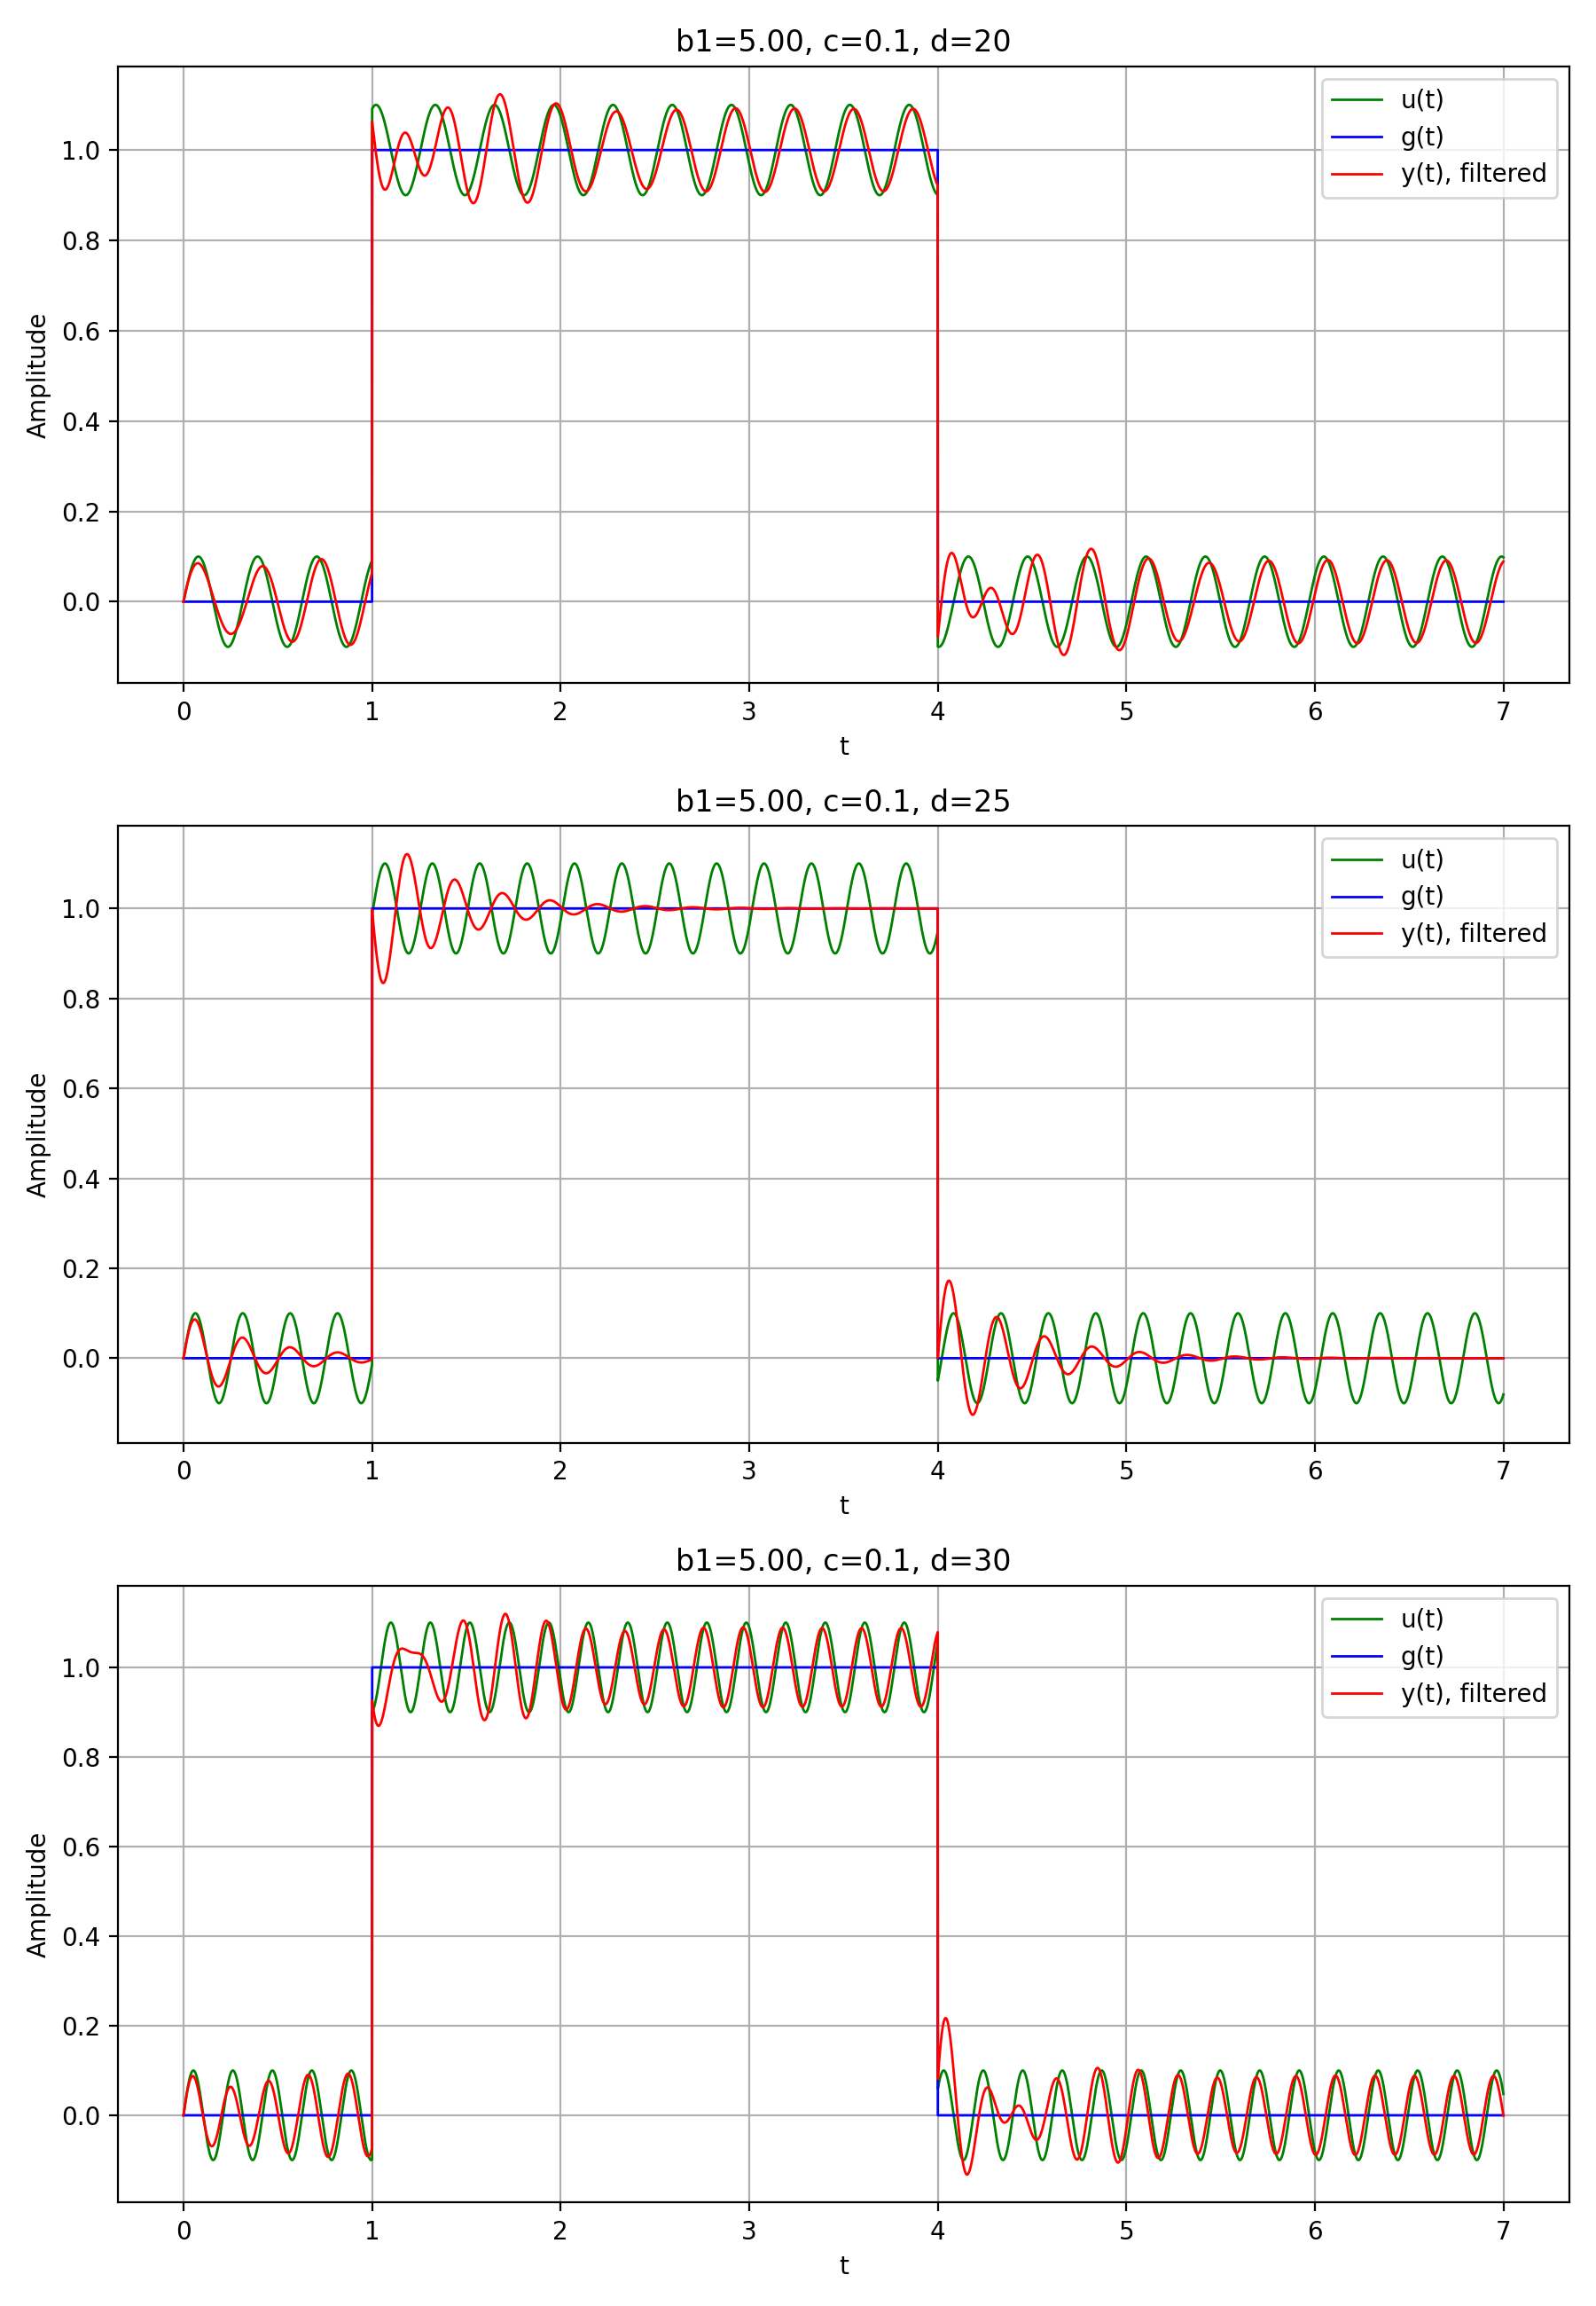
\includegraphics[width=1.0\linewidth]{fig/plots/Figure 14.png}
    \caption{Сигнал}
    \label{fig:14}
\end{figure}
\begin{figure}[H]
    \centering
    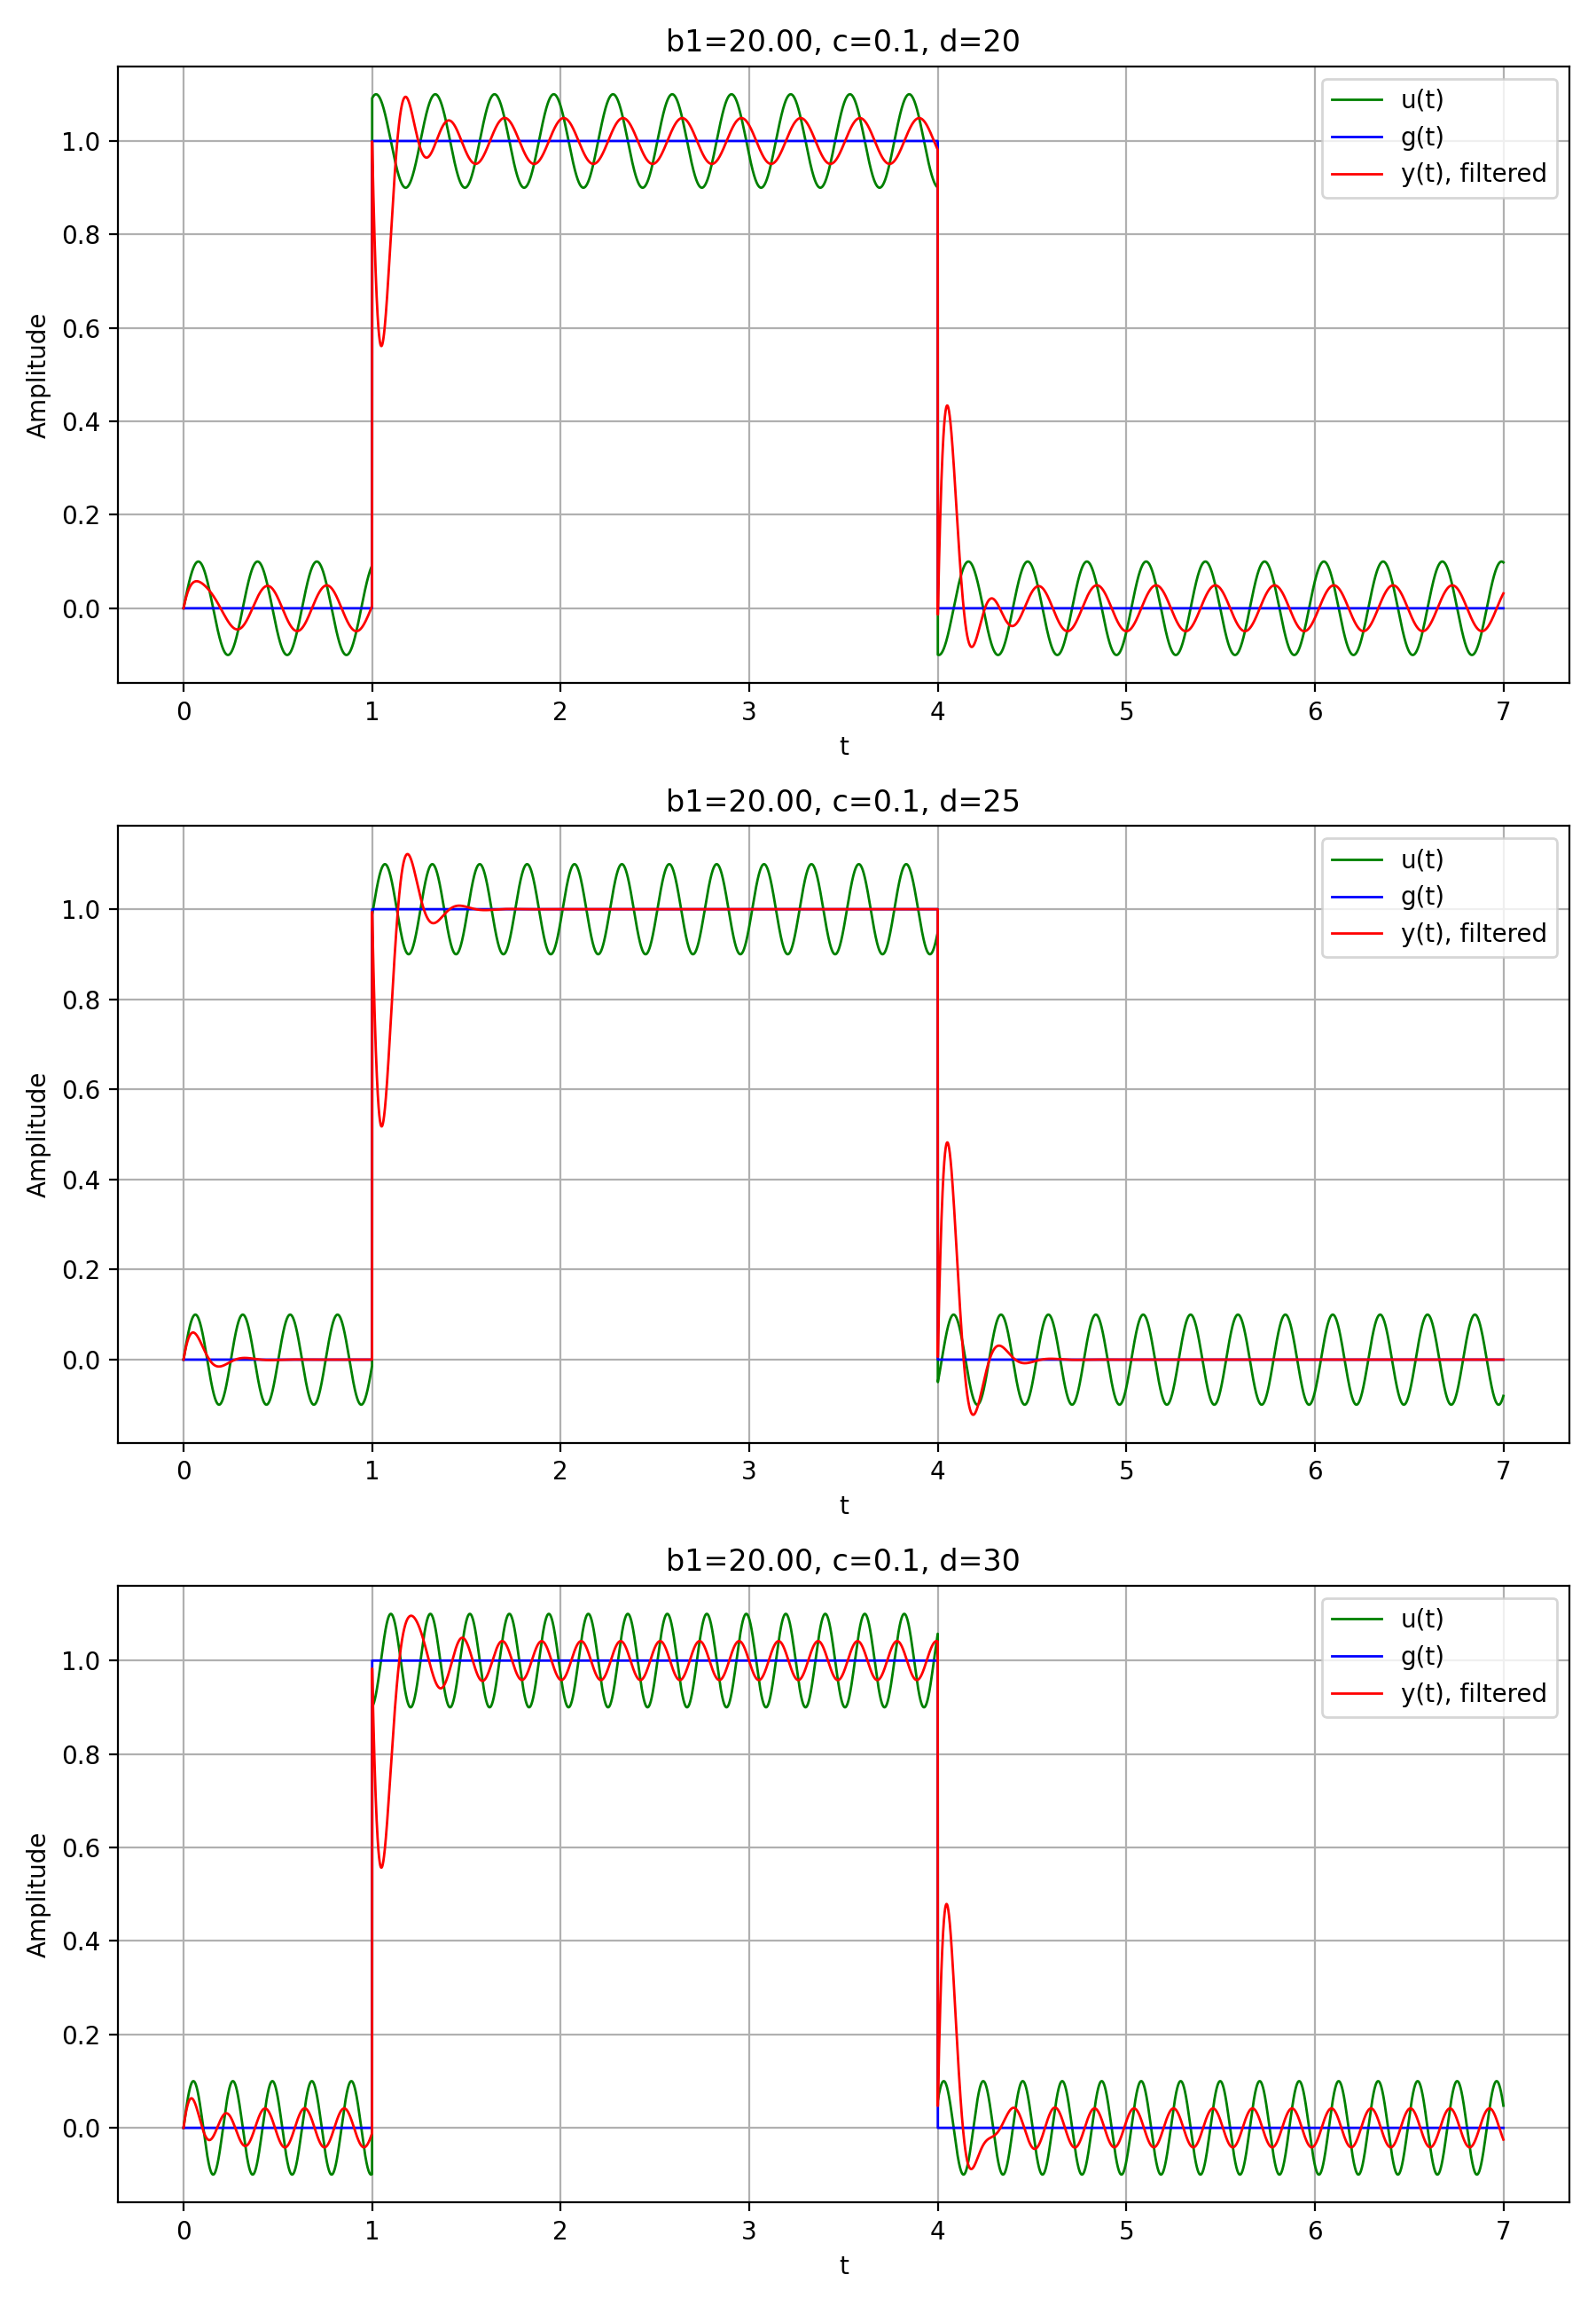
\includegraphics[width=1.0\linewidth]{fig/plots/Figure 15.png}
    \caption{Сигнал}
    \label{fig:15}
\end{figure}
\begin{figure}[H]
    \centering
    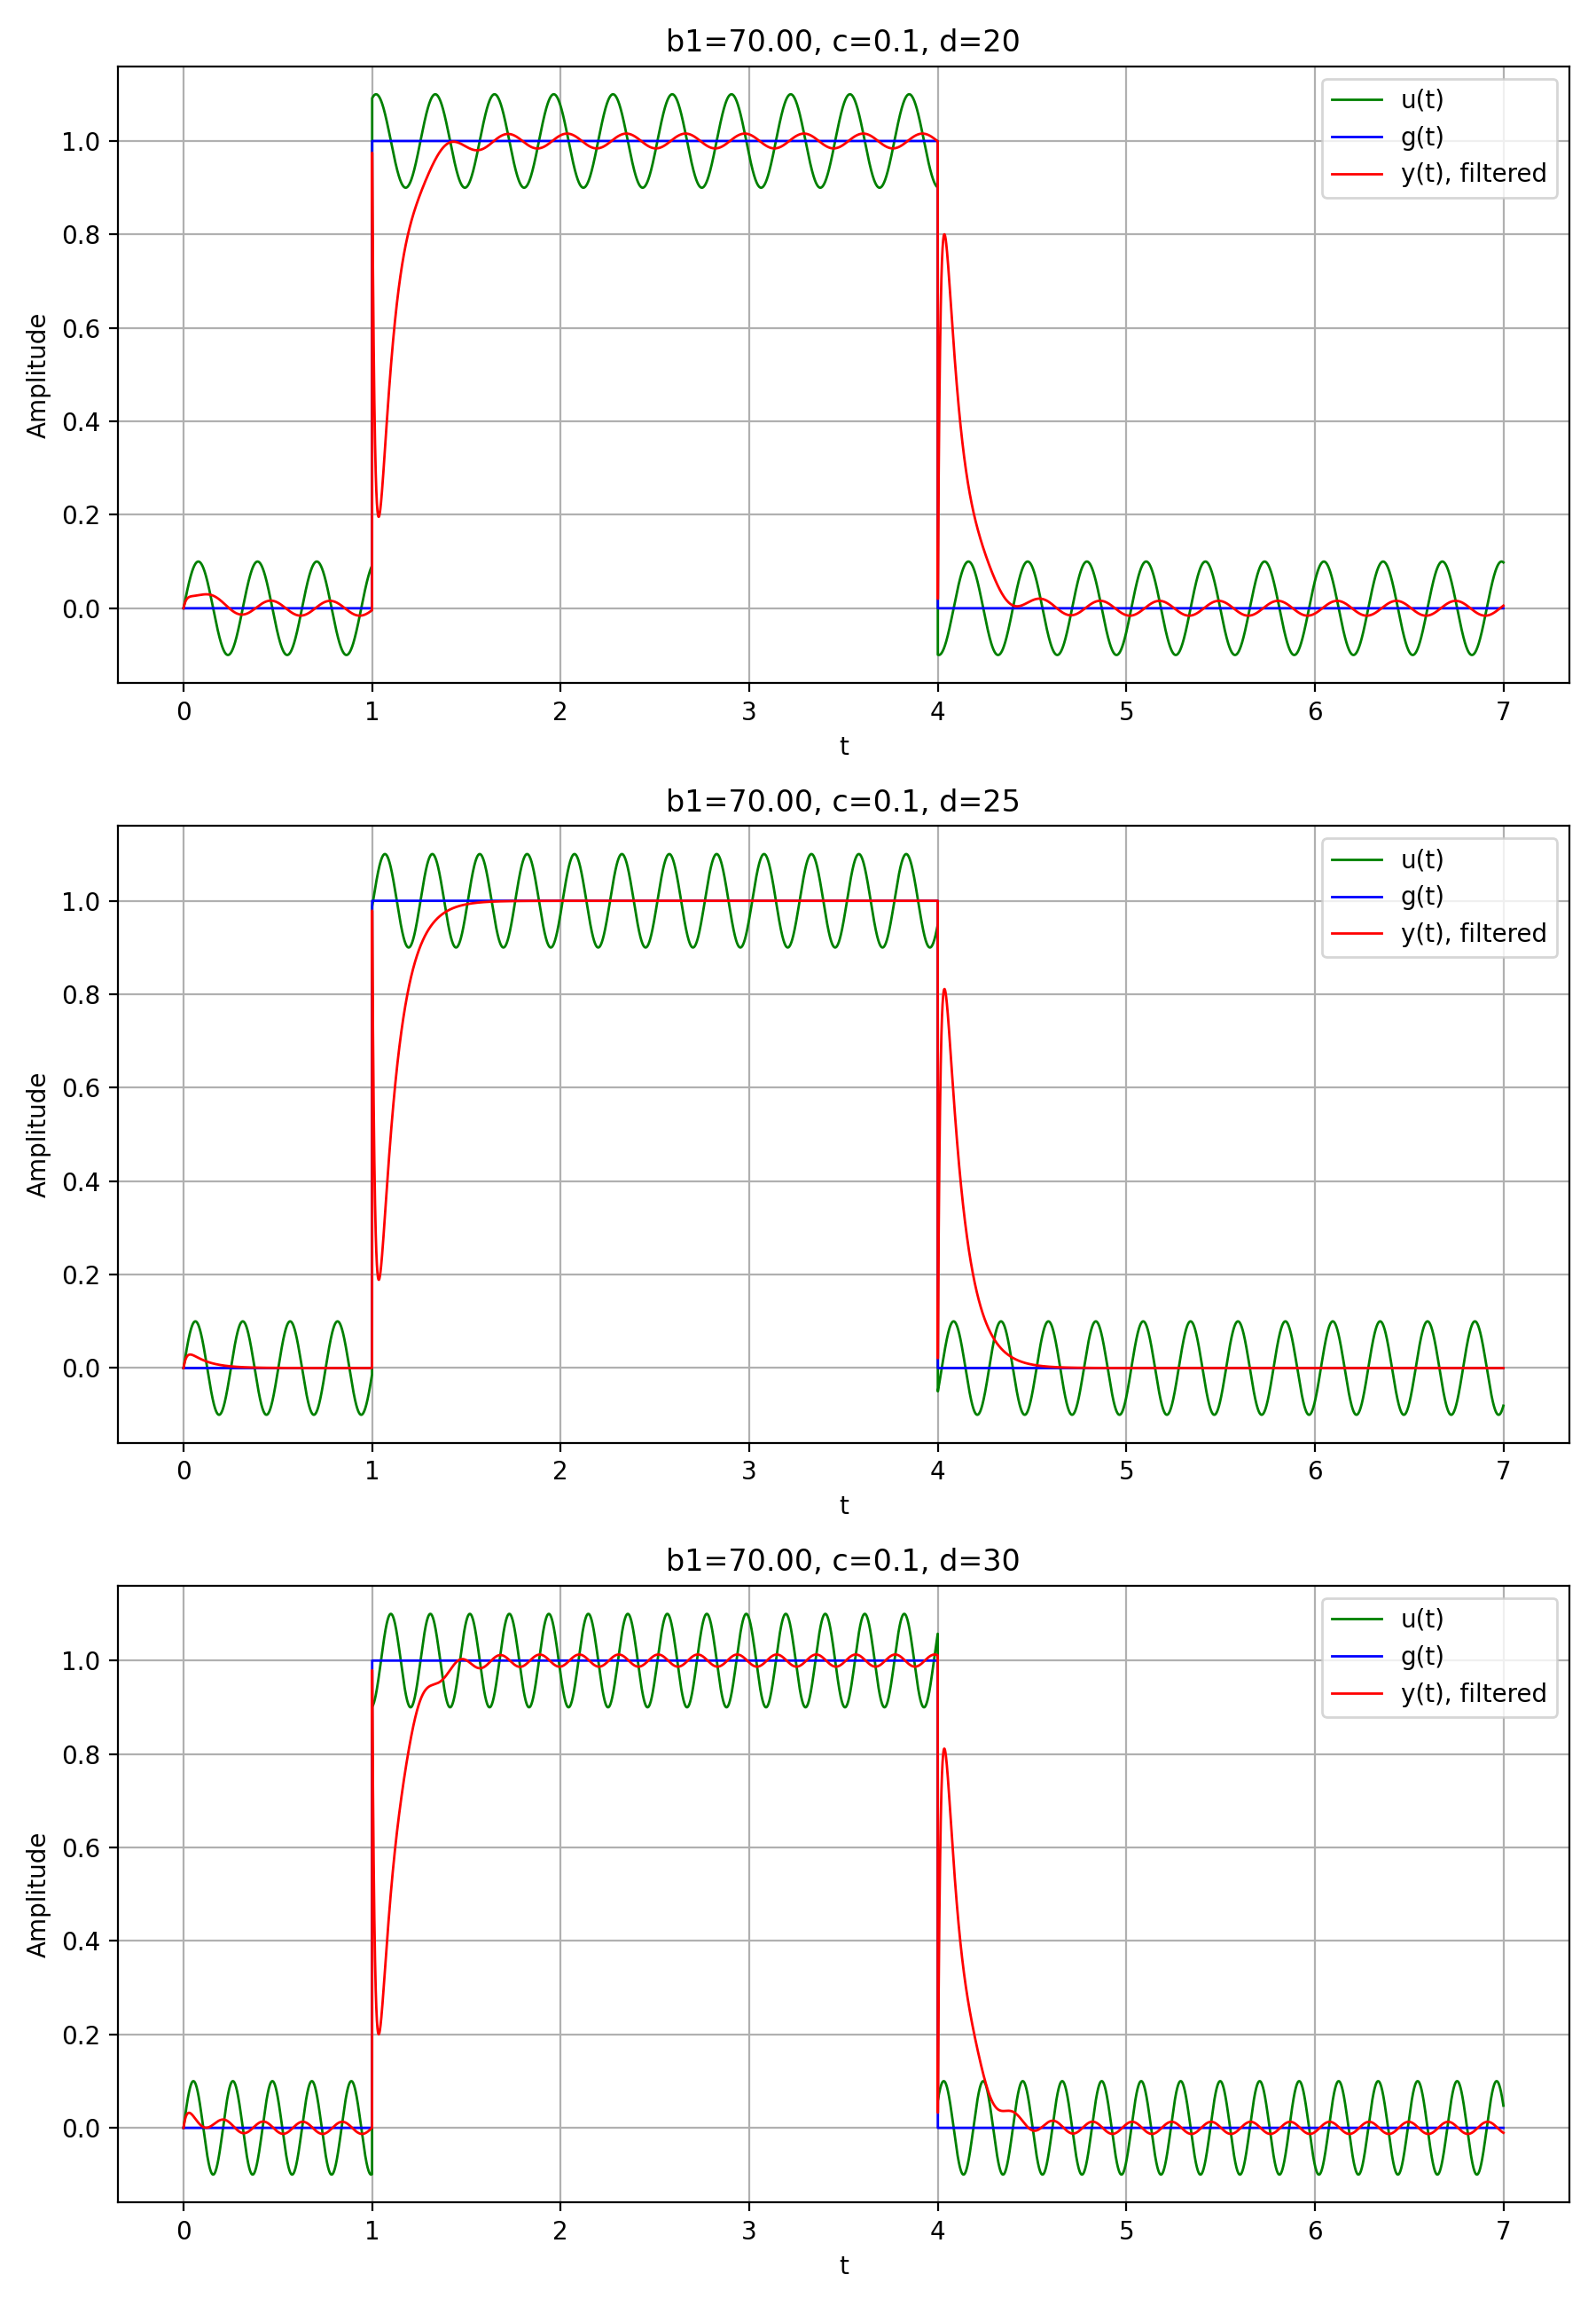
\includegraphics[width=1.0\linewidth]{fig/plots/Figure 16.png}
    \caption{Сигнал}
    \label{fig:16}
\end{figure}
\begin{figure}[H]
    \centering
    
\includegraphics[width=1.0\linewidth]{fig/plots/Figure 17.png}
    \caption{Сигнал}
    \label{fig:17}
\end{figure}
\begin{figure}[H]
    \centering
    
\includegraphics[width=1.0\linewidth]{fig/plots/Figure 18.png}
    \caption{Сигнал}
    \label{fig:18}
\end{figure}
\begin{figure}[H]
    \centering
    
\includegraphics[width=1.0\linewidth]{fig/plots/Figure 19.png}
    \caption{Сигнал}
    \label{fig:19}
\end{figure}
\begin{figure}[H]
    \centering
    
\includegraphics[width=1.0\linewidth]{fig/plots/Figure 20.png}
    \caption{Сигнал}
    \label{fig:20}
\end{figure}
\begin{figure}[H]
    \centering
    
\includegraphics[width=1.0\linewidth]{fig/plots/Figure 21.png}
    \caption{Сигнал}
    \label{fig:21}
\end{figure}

\begin{figure}[H]
    \centering
    
\includegraphics[width=1.0\linewidth]{fig/plots/Figure 22.png}
    \caption{Фурье-образ}
    \label{fig:22}
\end{figure}
\begin{figure}[H]
    \centering
    
\includegraphics[width=1.0\linewidth]{fig/plots/Figure 23.png}
    \caption{Фурье-образ}
    \label{fig:23}
\end{figure}
\begin{figure}[H]
    \centering
    
\includegraphics[width=1.0\linewidth]{fig/plots/Figure 24.png}
    \caption{Фурье-образ}
    \label{fig:24}
\end{figure}
\begin{figure}[H]
    \centering
    
\includegraphics[width=1.0\linewidth]{fig/plots/Figure 25.png}
    \caption{Фурье-образ}
    \label{fig:25}
\end{figure}
\begin{figure}[H]
    \centering
    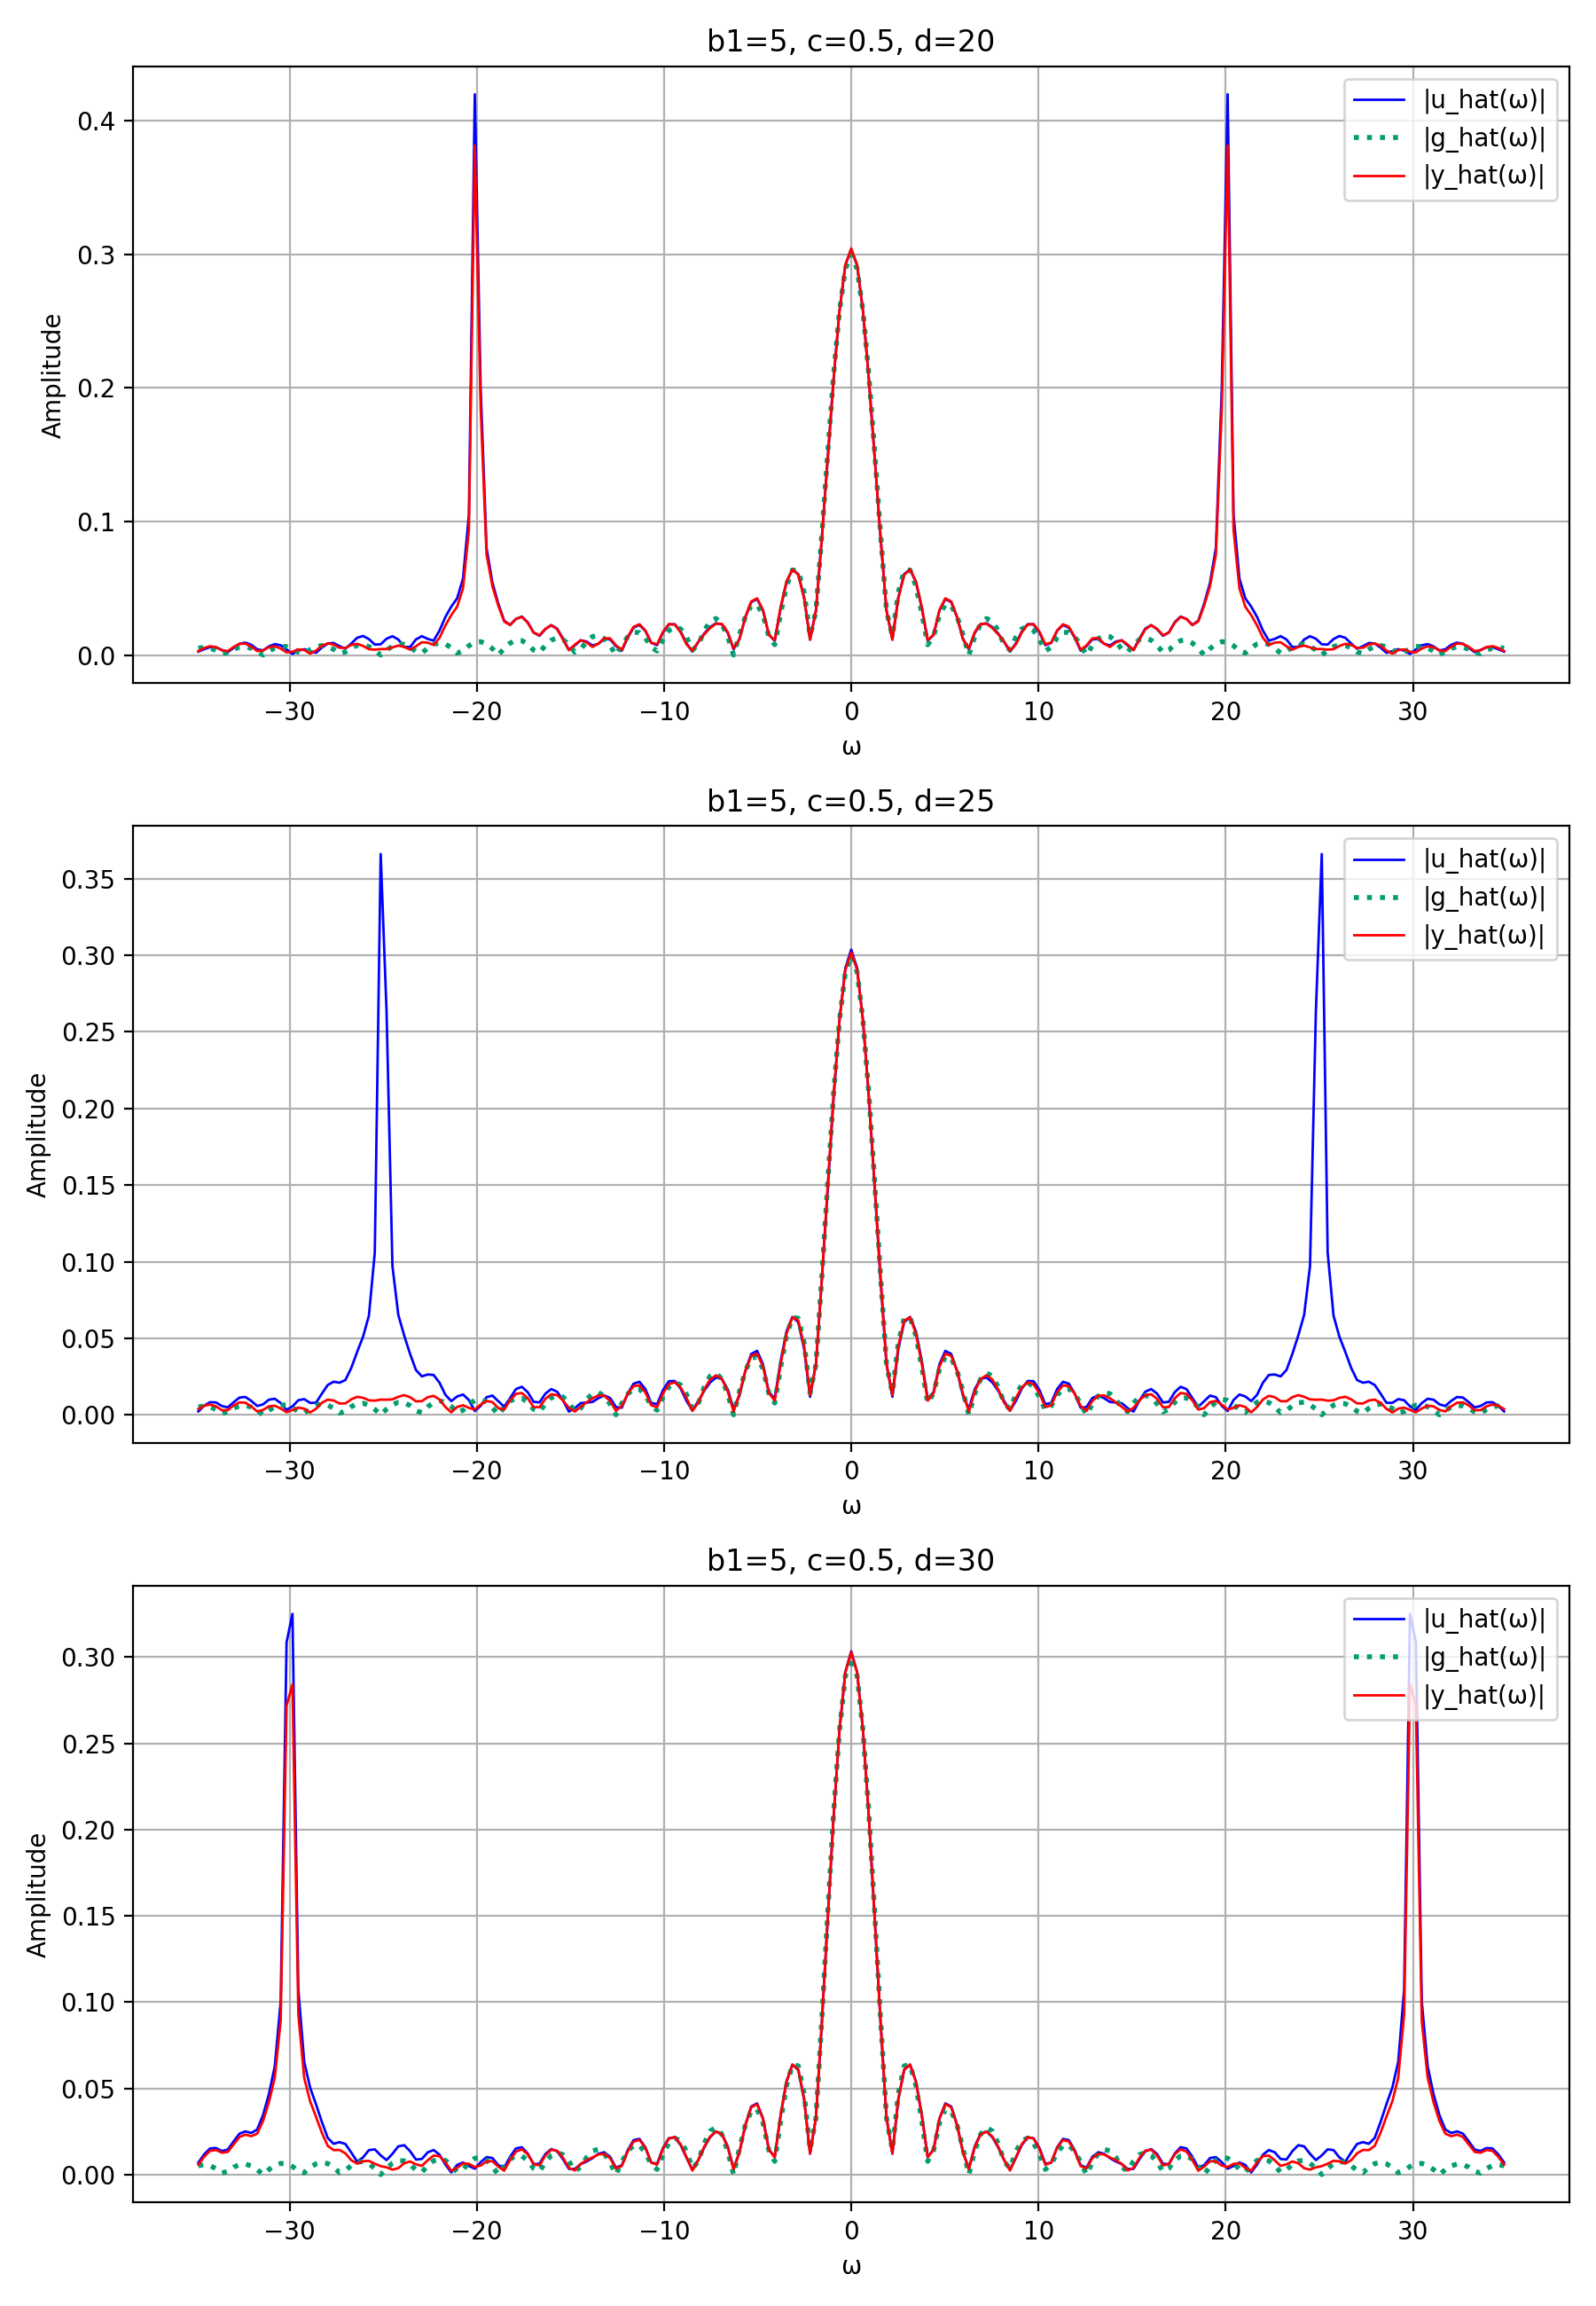
\includegraphics[width=1.0\linewidth]{fig/plots/Figure 26.png}
    \caption{Фурье-образ}
    \label{fig:26}
\end{figure}
\begin{figure}[H]
    \centering
    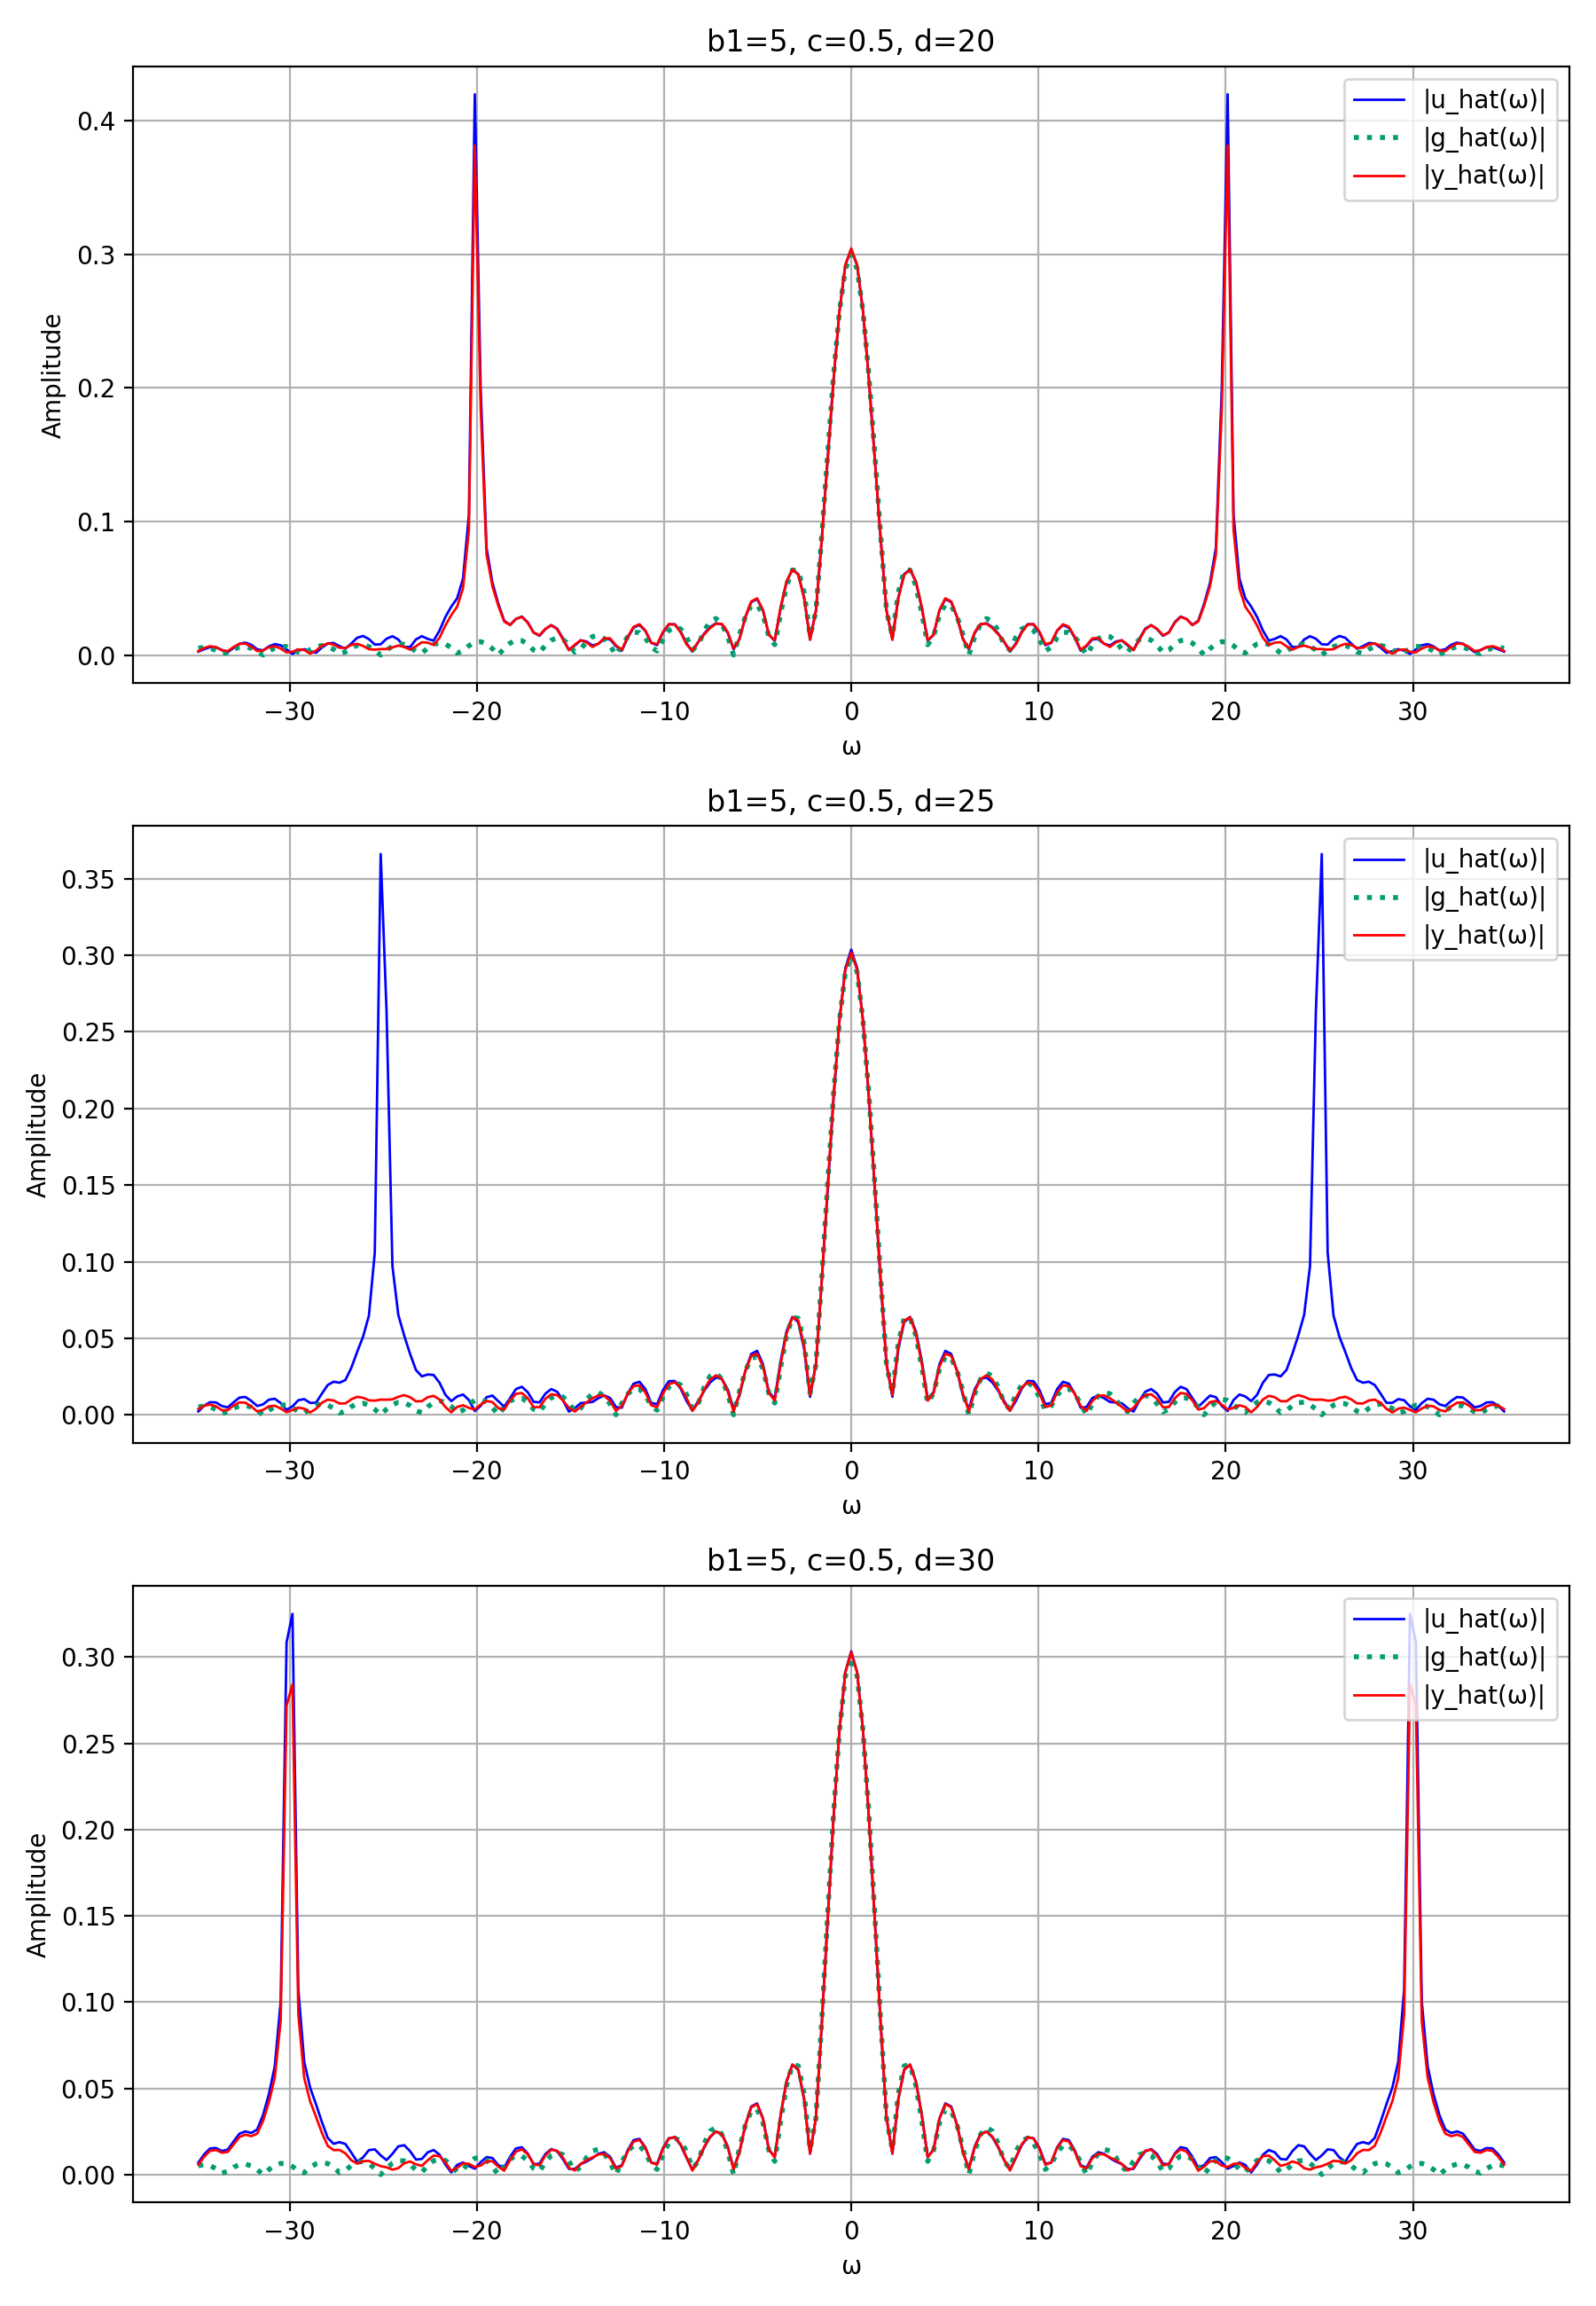
\includegraphics[width=1.0\linewidth]{fig/plots/Figure 26.png}
    \caption{Фурье-образ}
    \label{fig:27}
\end{figure}
\begin{figure}[H]
    \centering
    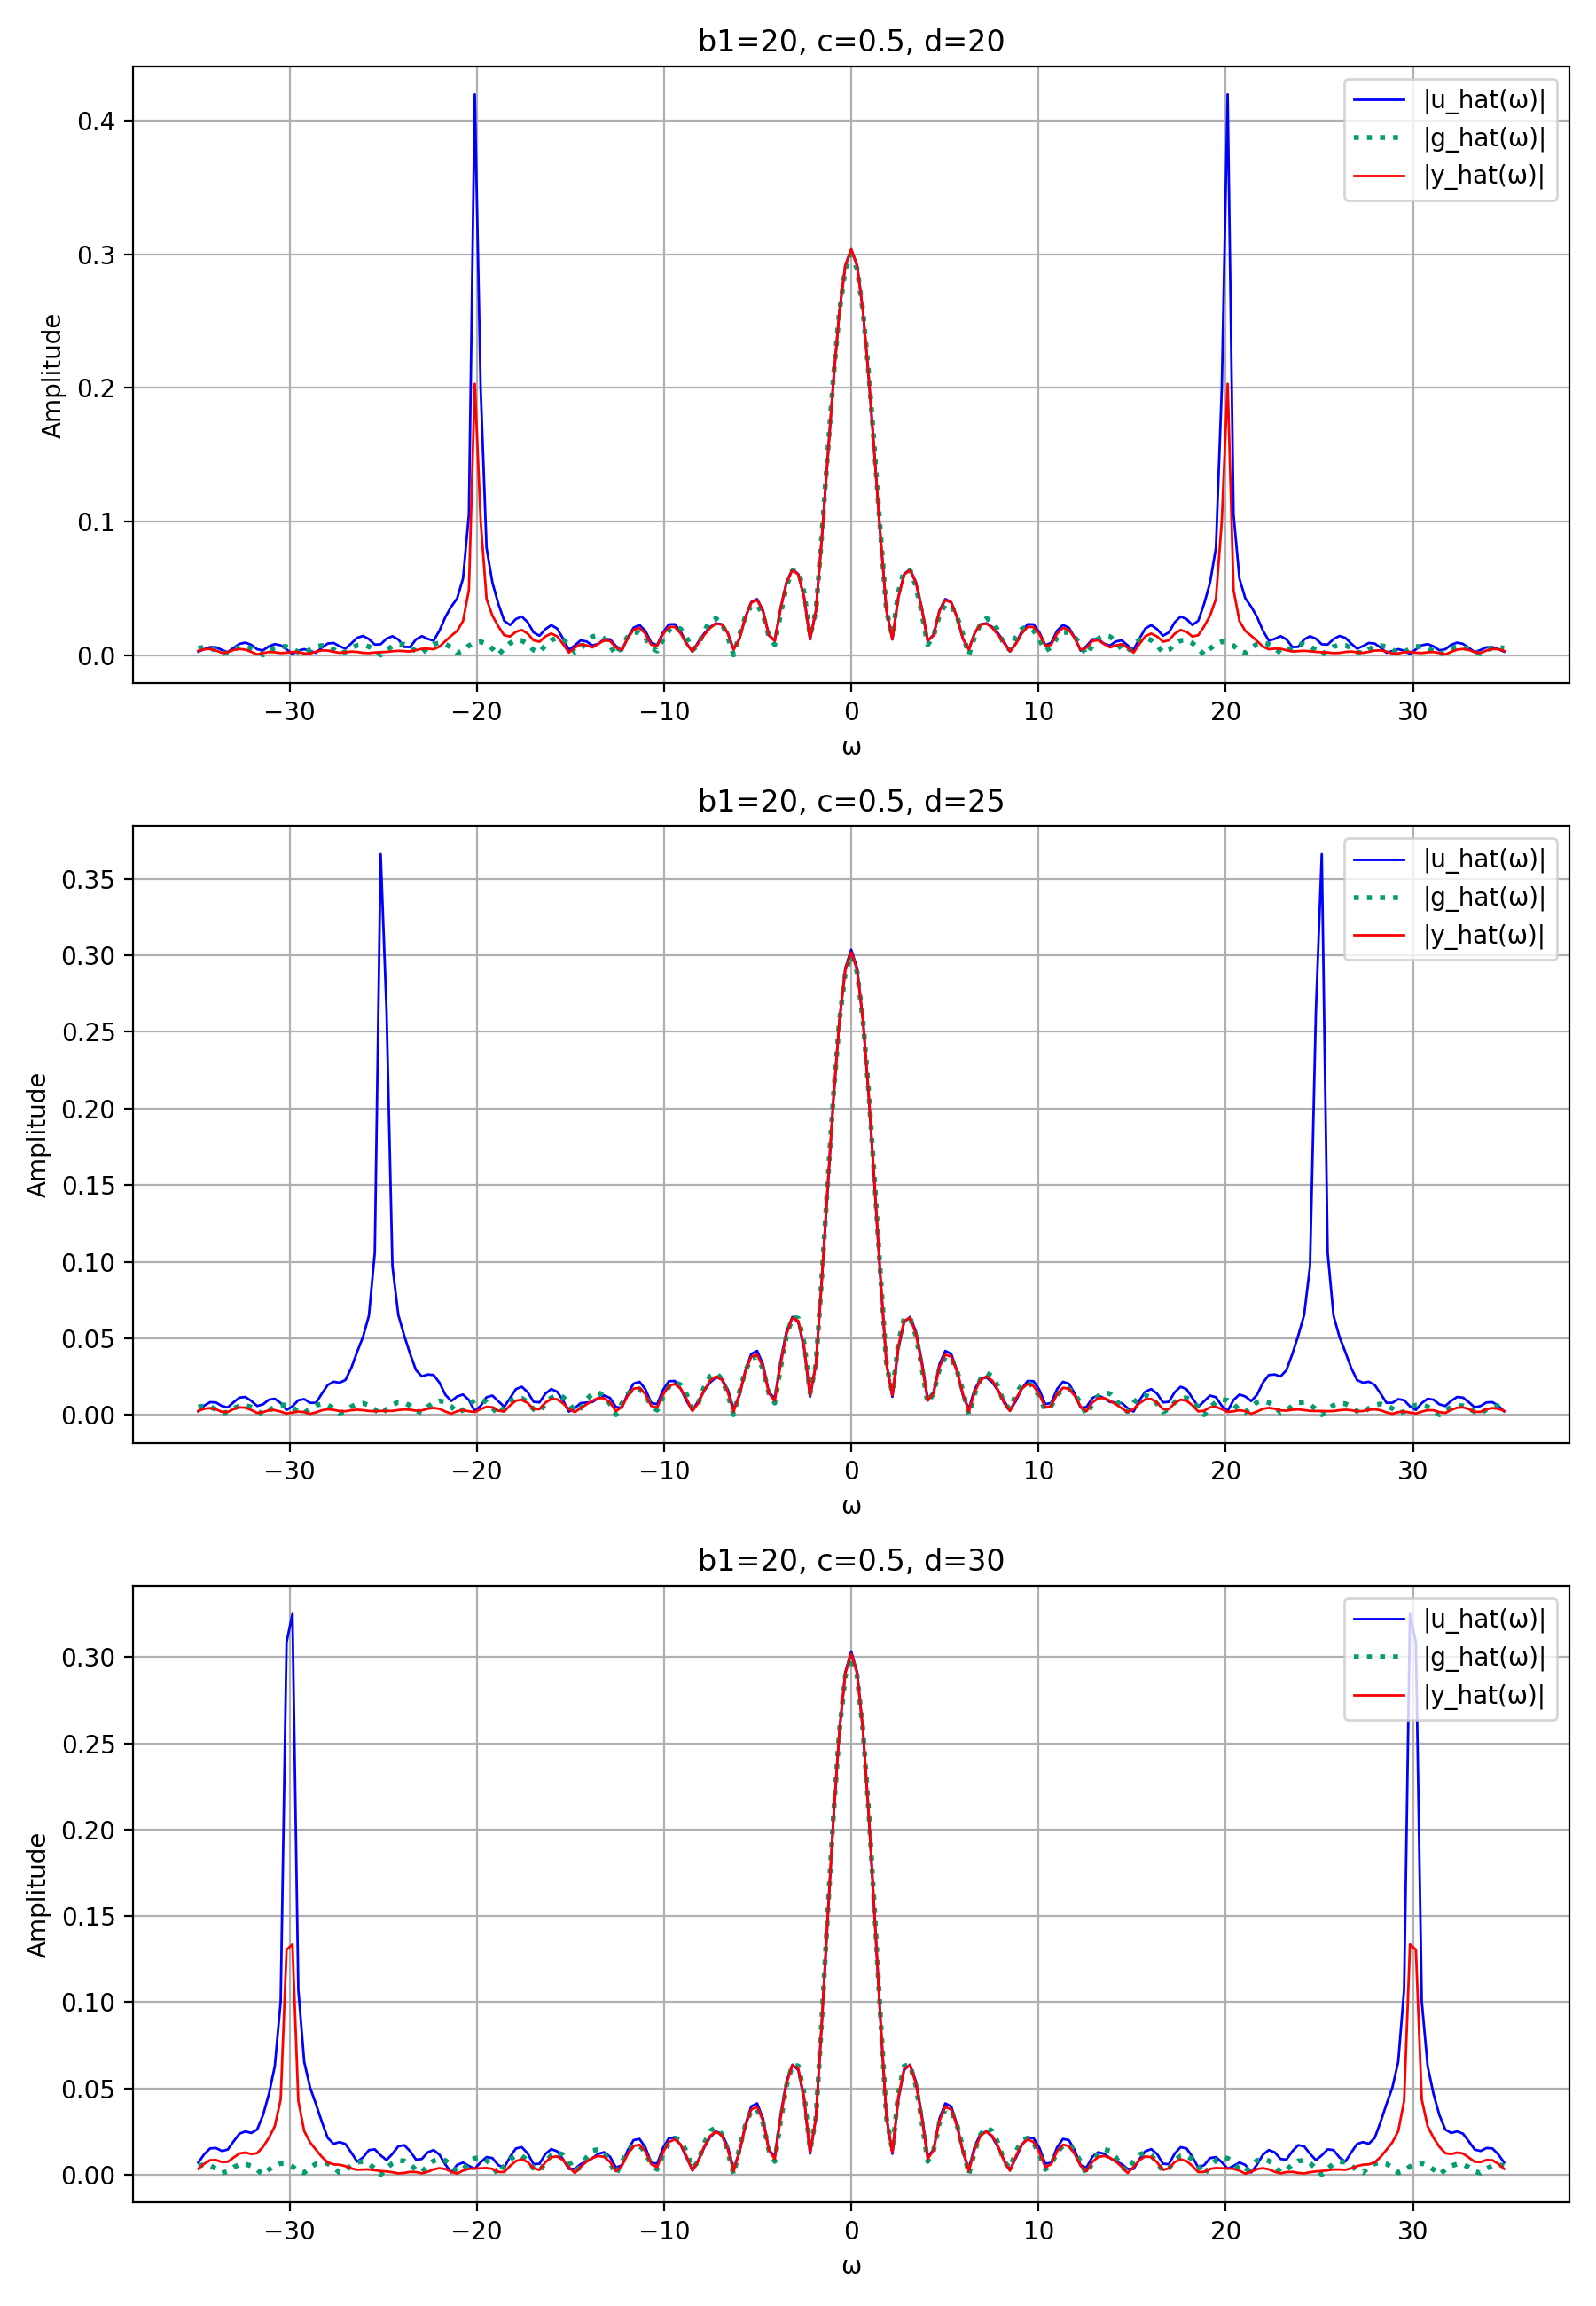
\includegraphics[width=1.0\linewidth]{fig/plots/Figure 27.png}
    \caption{Фурье-образ}
    \label{fig:28}
\end{figure}
\begin{figure}[H]
    \centering
    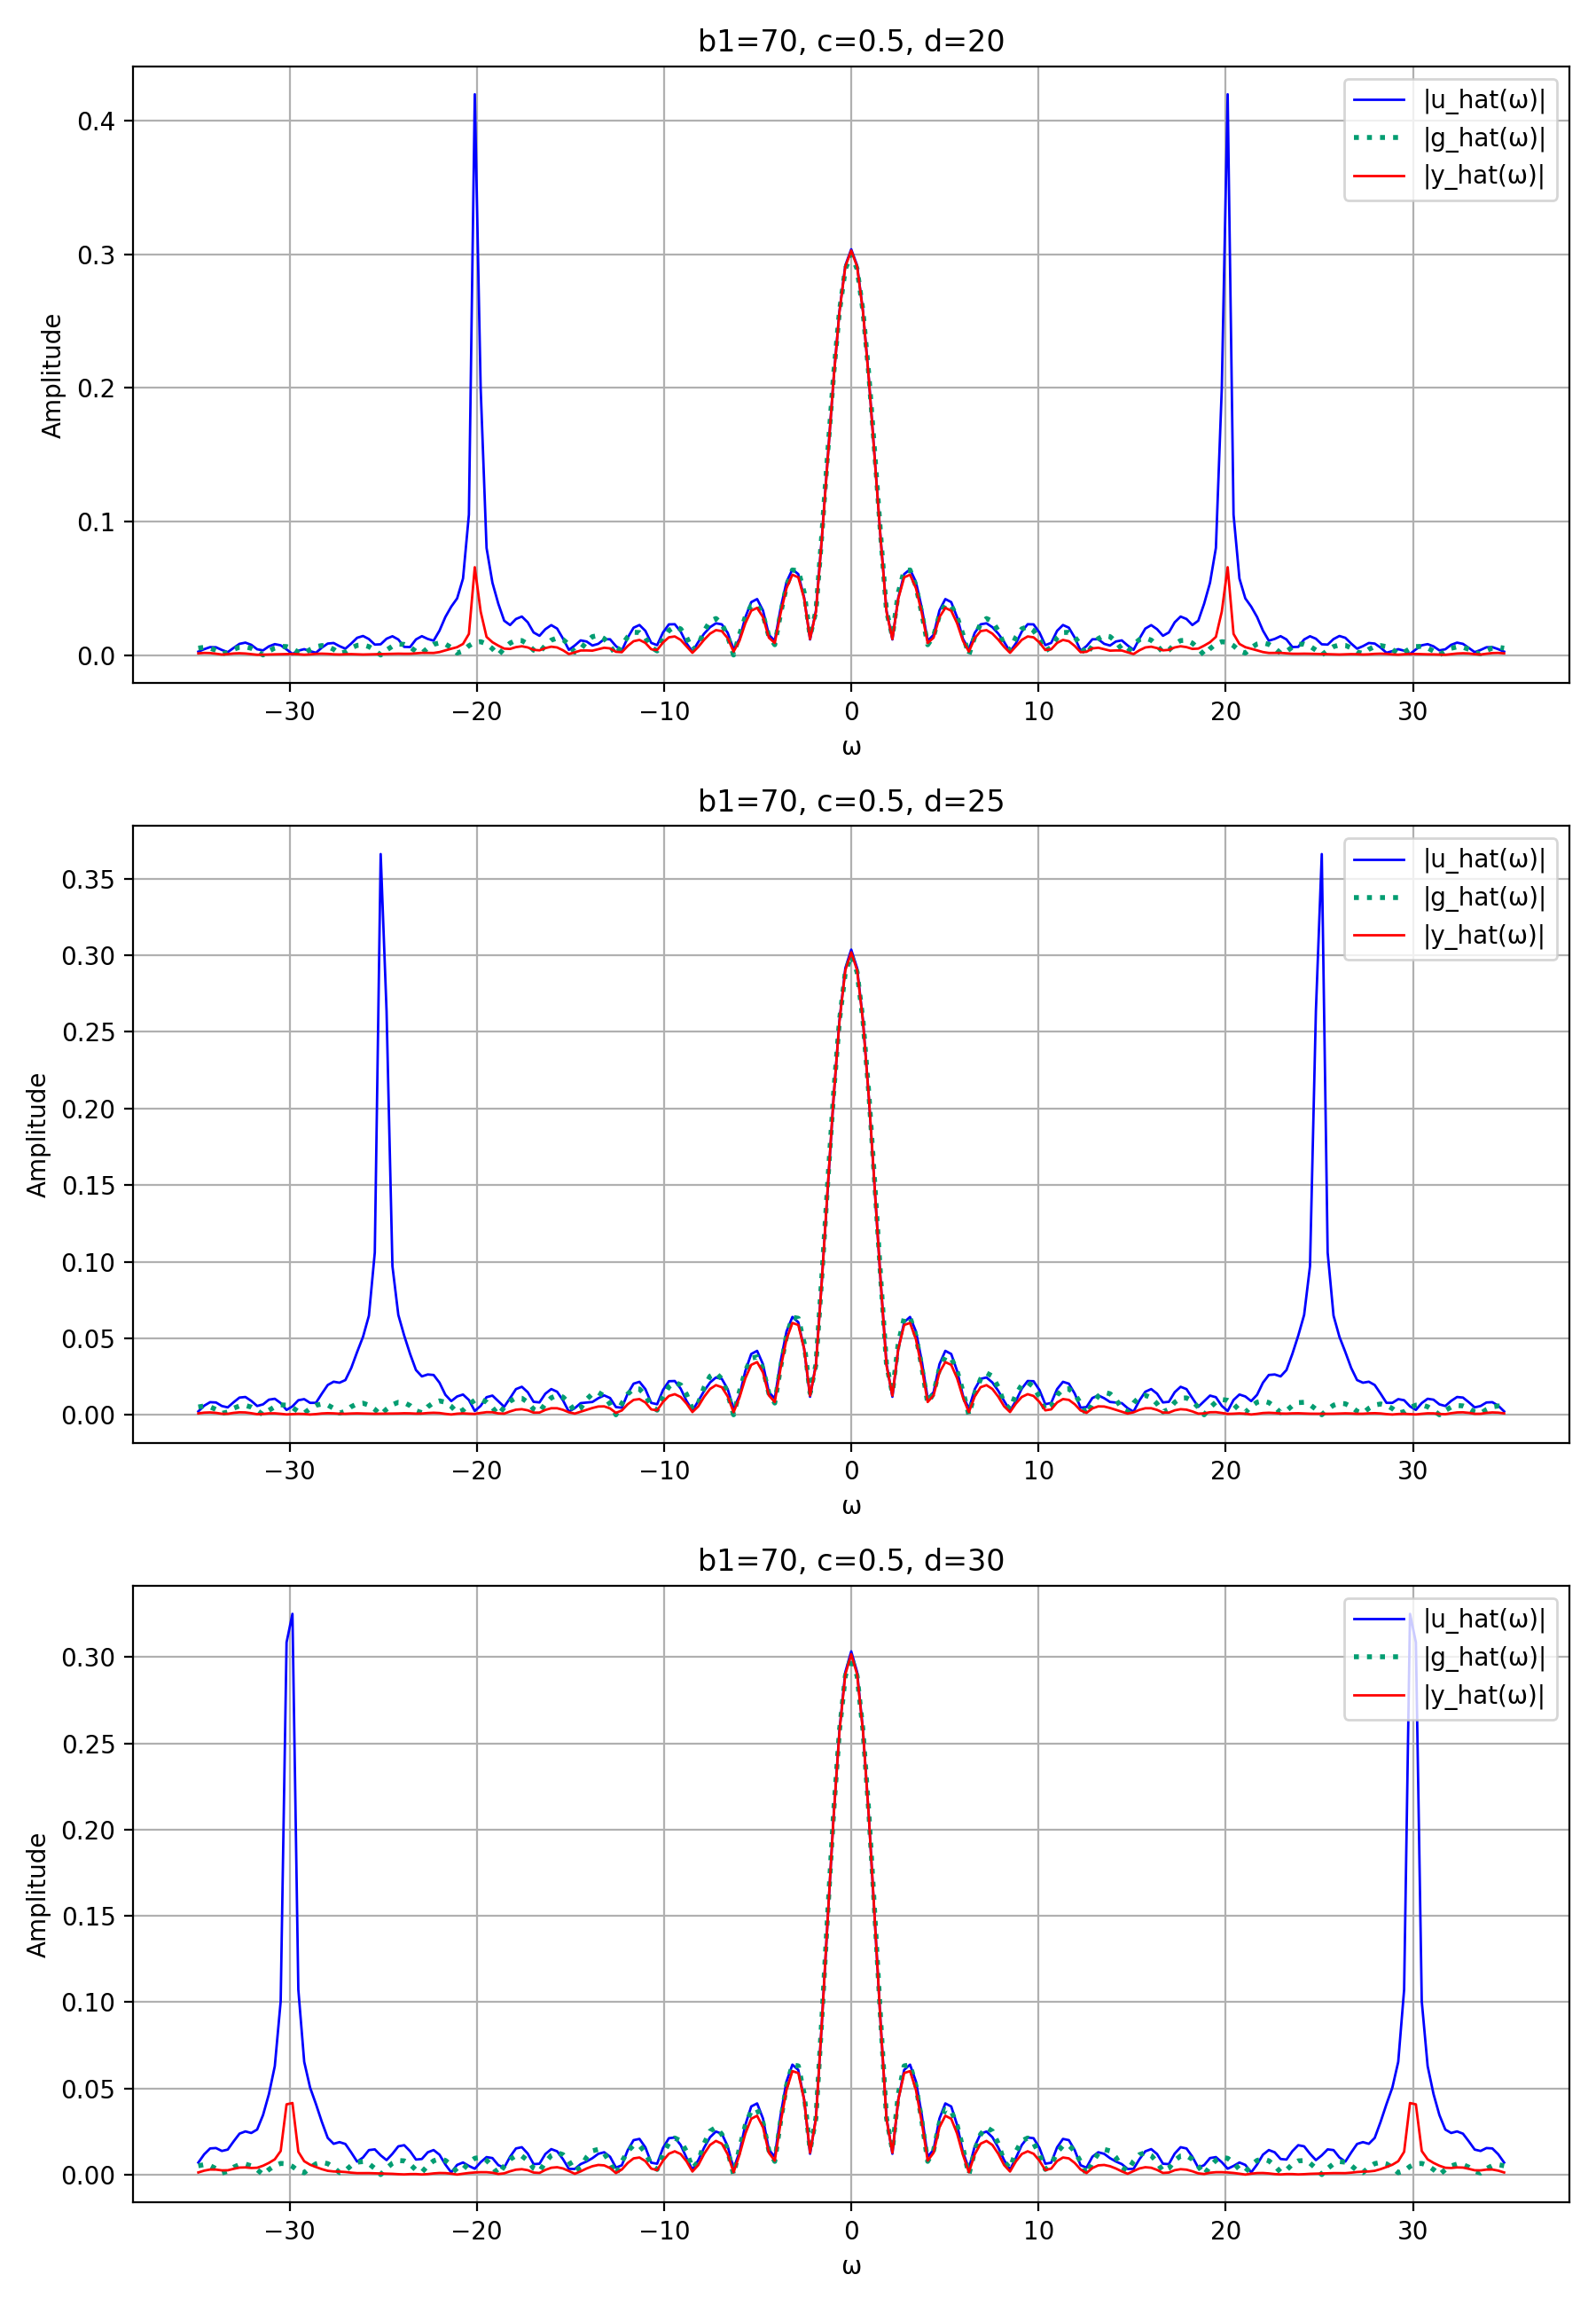
\includegraphics[width=1.0\linewidth]{fig/plots/Figure 28.png}
    \caption{Фурье-образ}
    \label{fig:29}
\end{figure}

\begin{figure}[H]
    \centering
    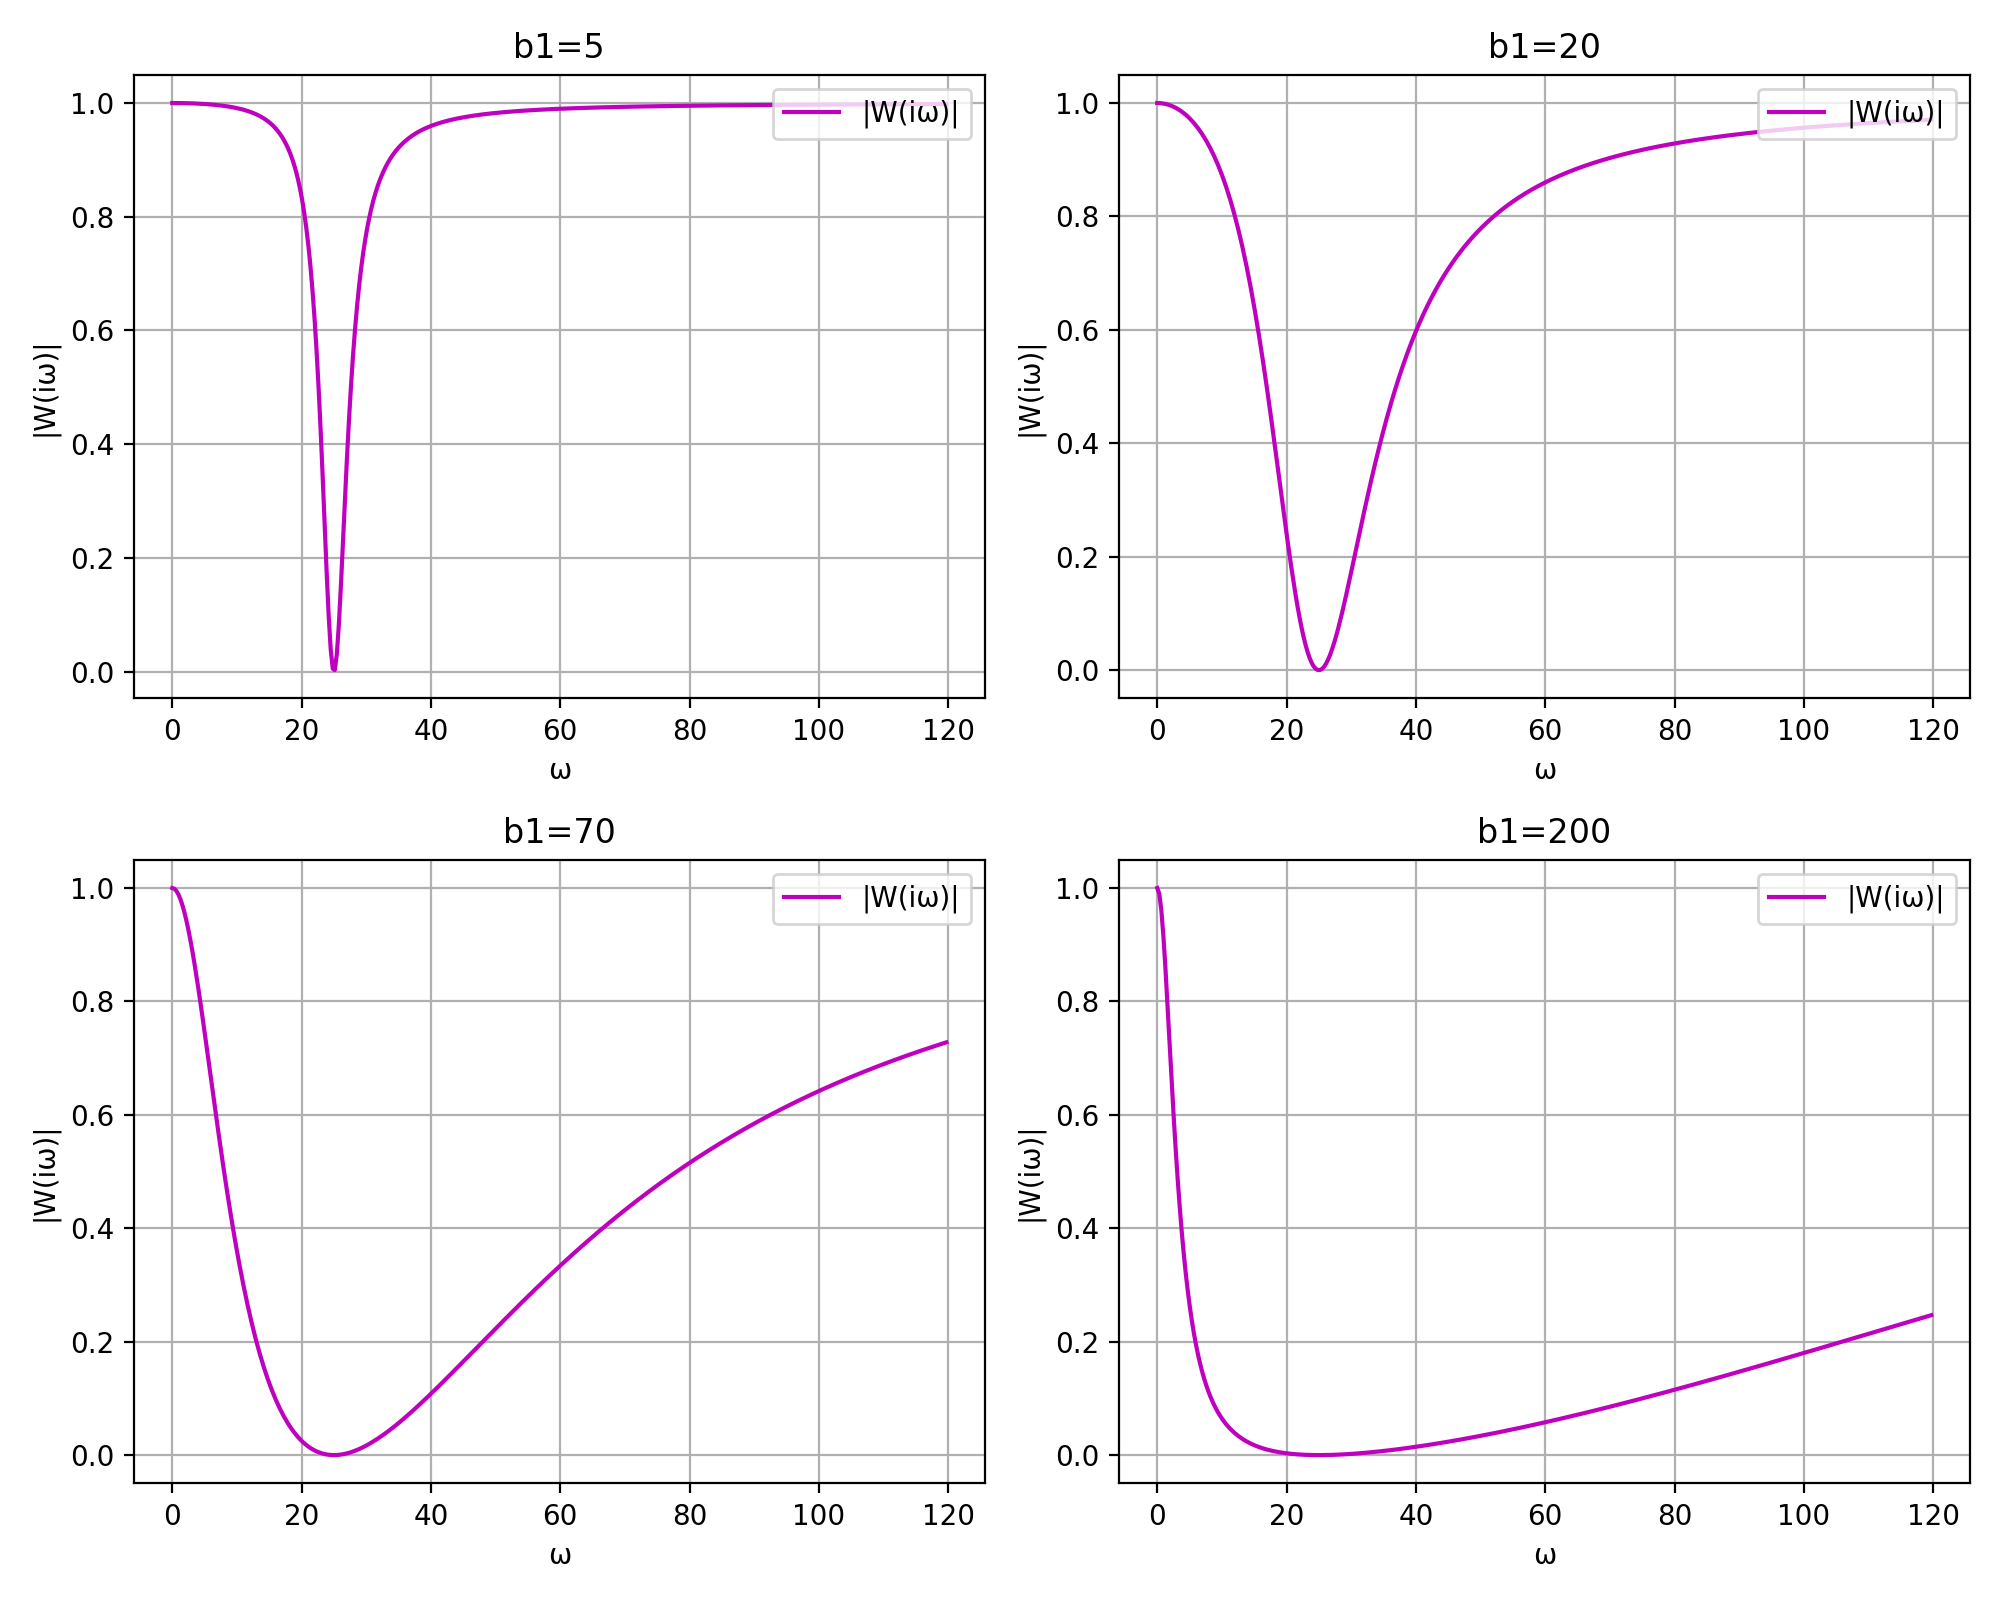
\includegraphics[width=1.0\linewidth]{fig/plots/Figure 30.png}
    \caption{АЧХ}
    \label{fig:30}
\end{figure}

\begin{figure}[H]
    \centering
    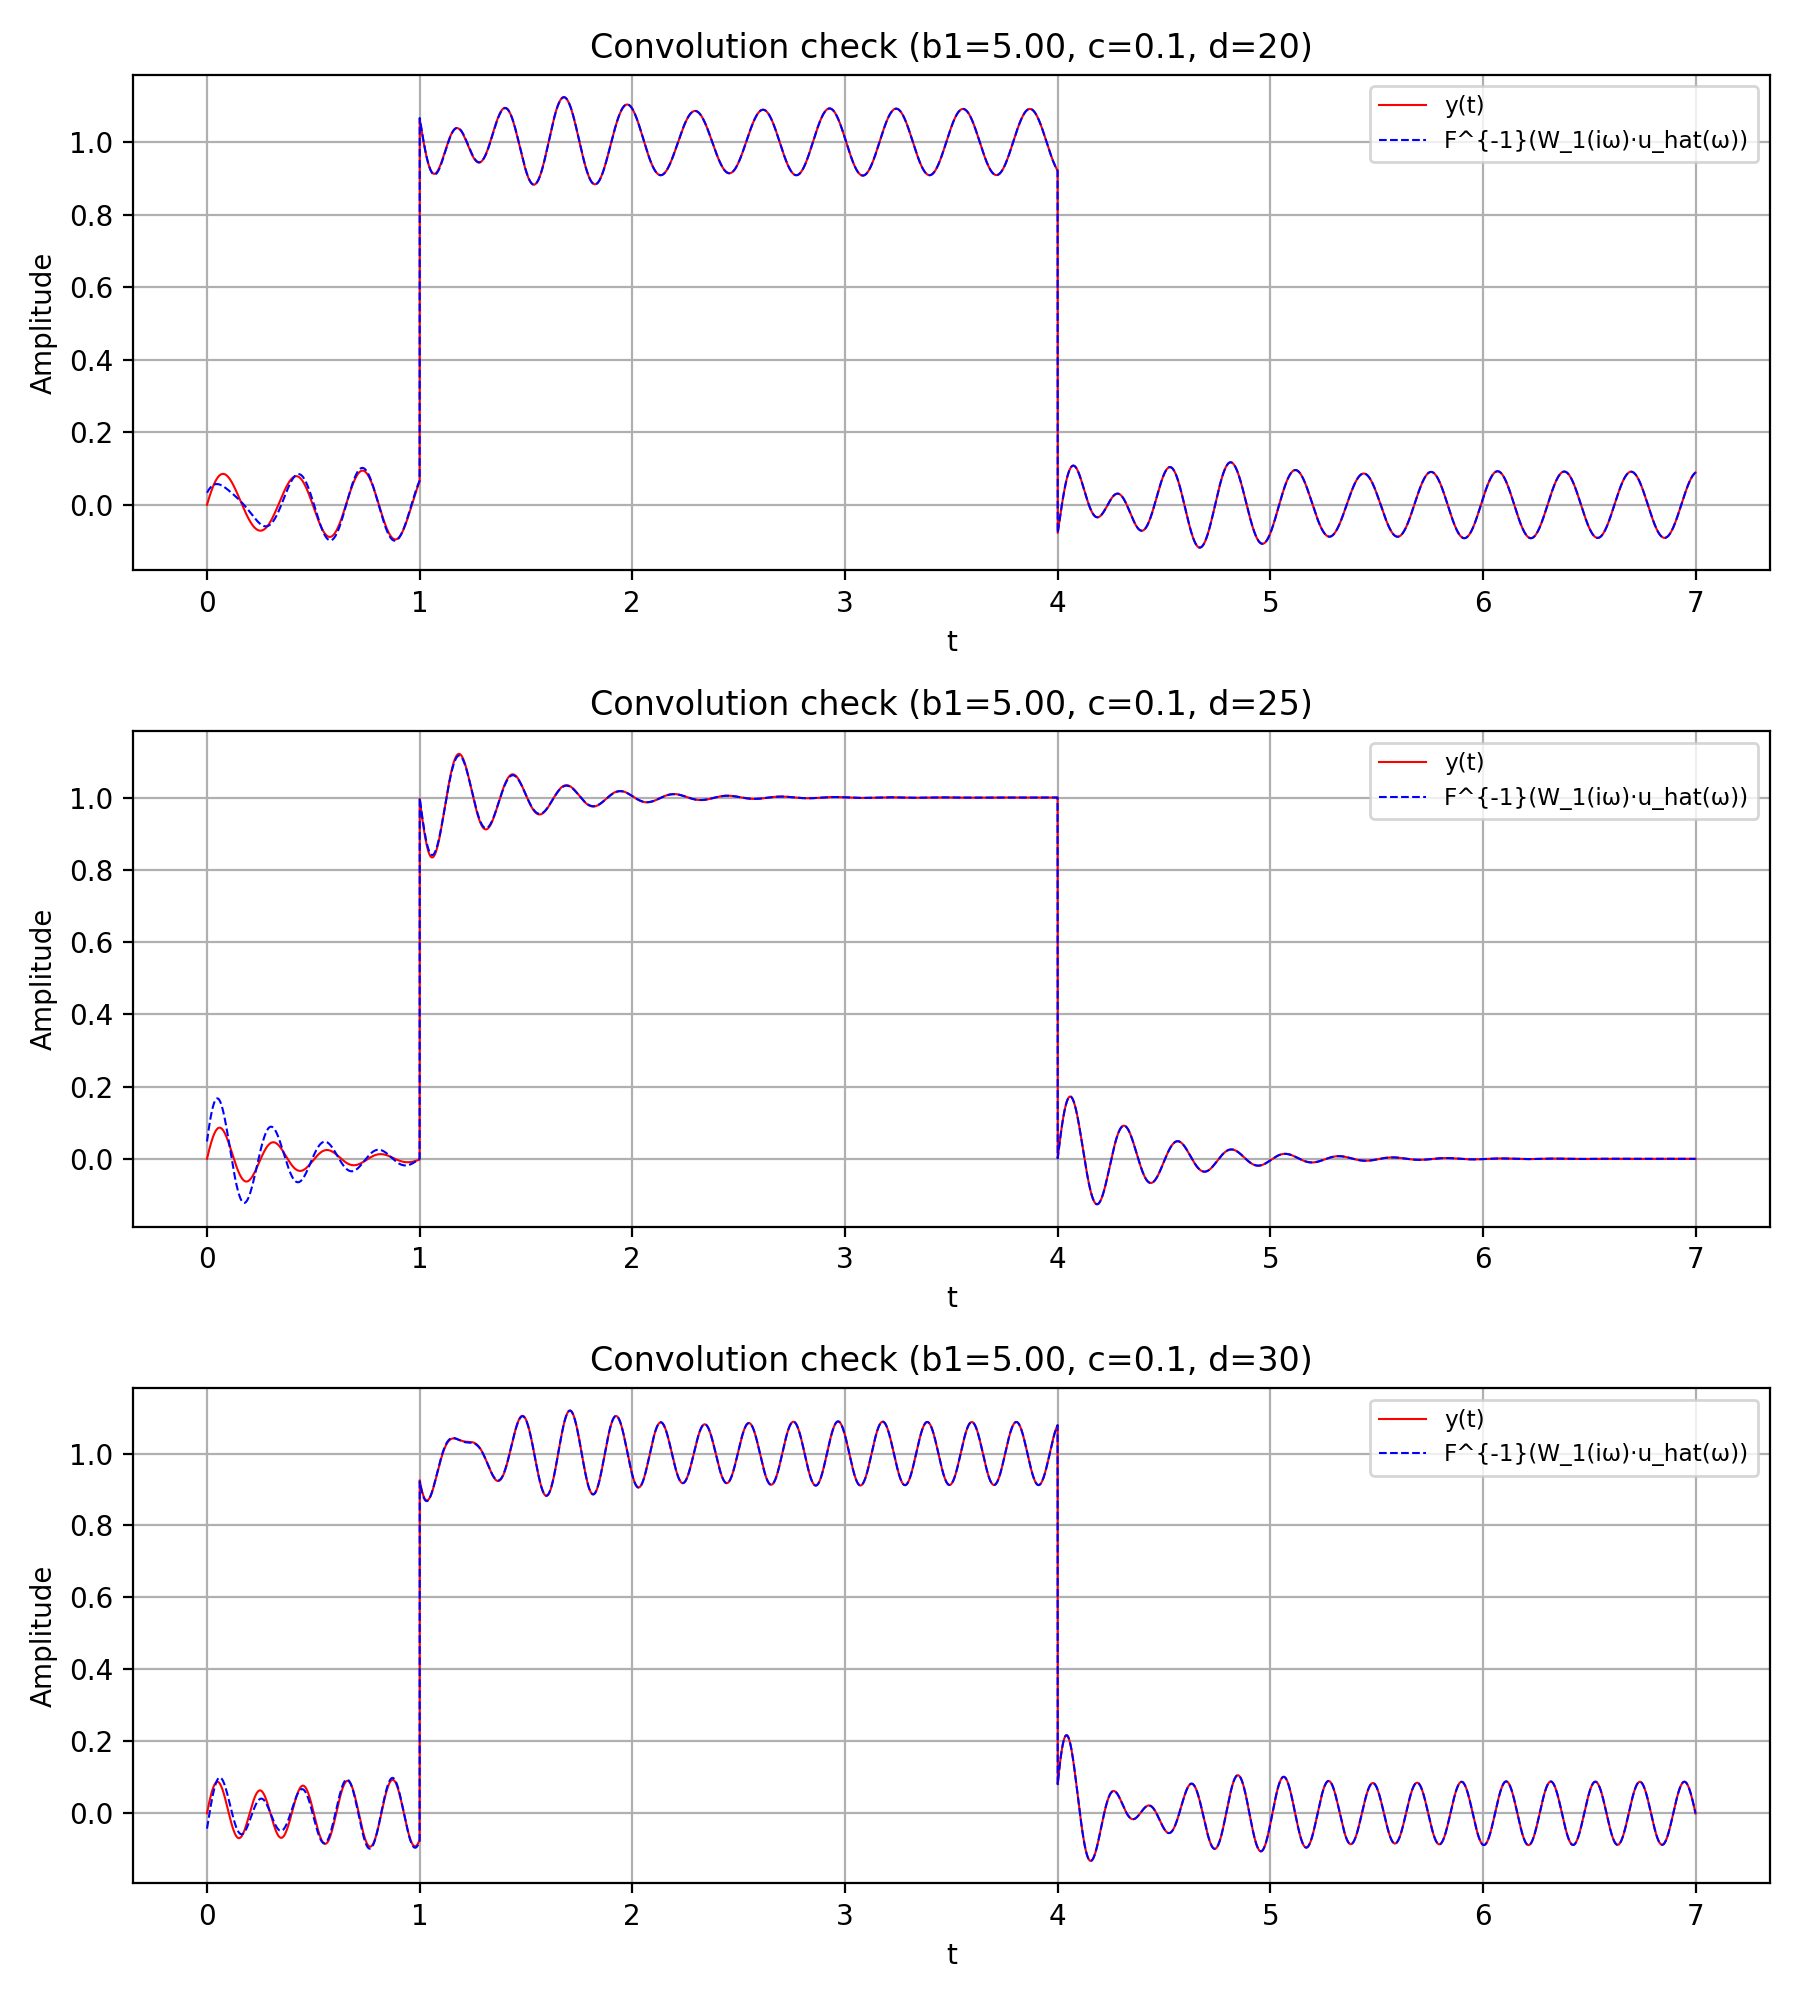
\includegraphics[width=1.0\linewidth]{fig/plots/Figure 31.png}
    \caption{Временная область}
    \label{fig:31}
\end{figure}
\begin{figure}[H]
    \centering
    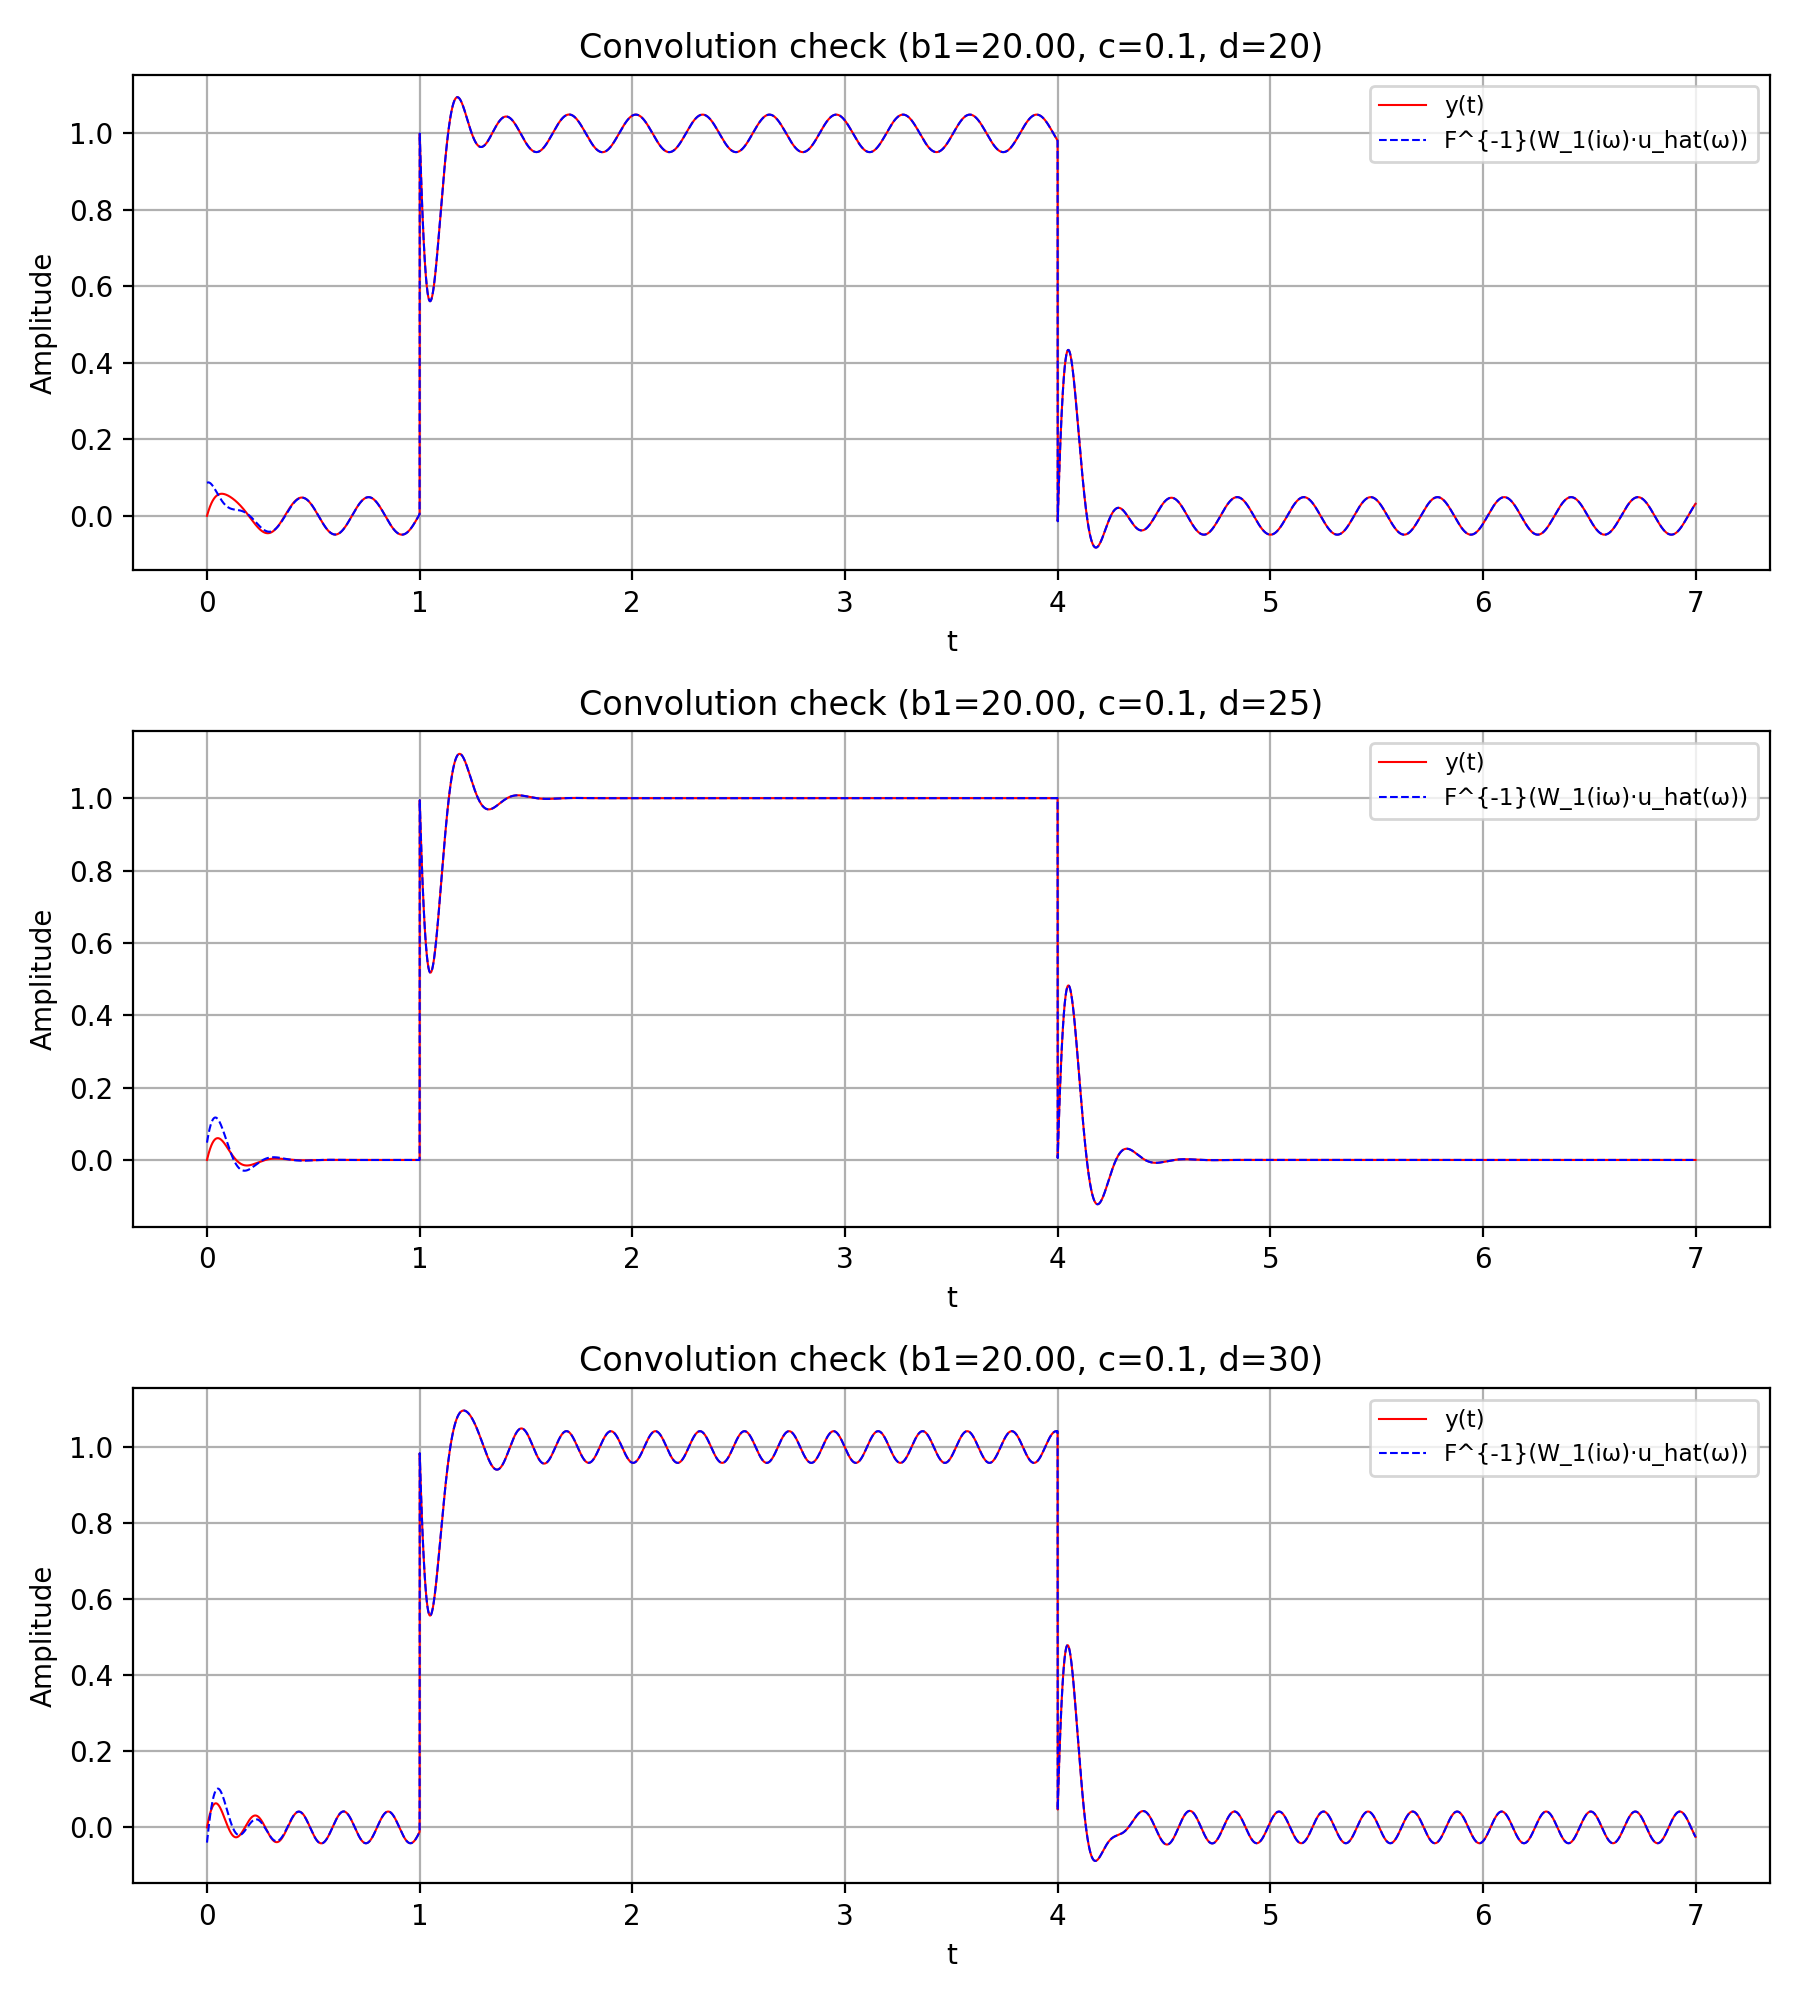
\includegraphics[width=1.0\linewidth]{fig/plots/Figure 32.png}
    \caption{Временная область}
    \label{fig:32}
\end{figure}
\begin{figure}[H]
    \centering
    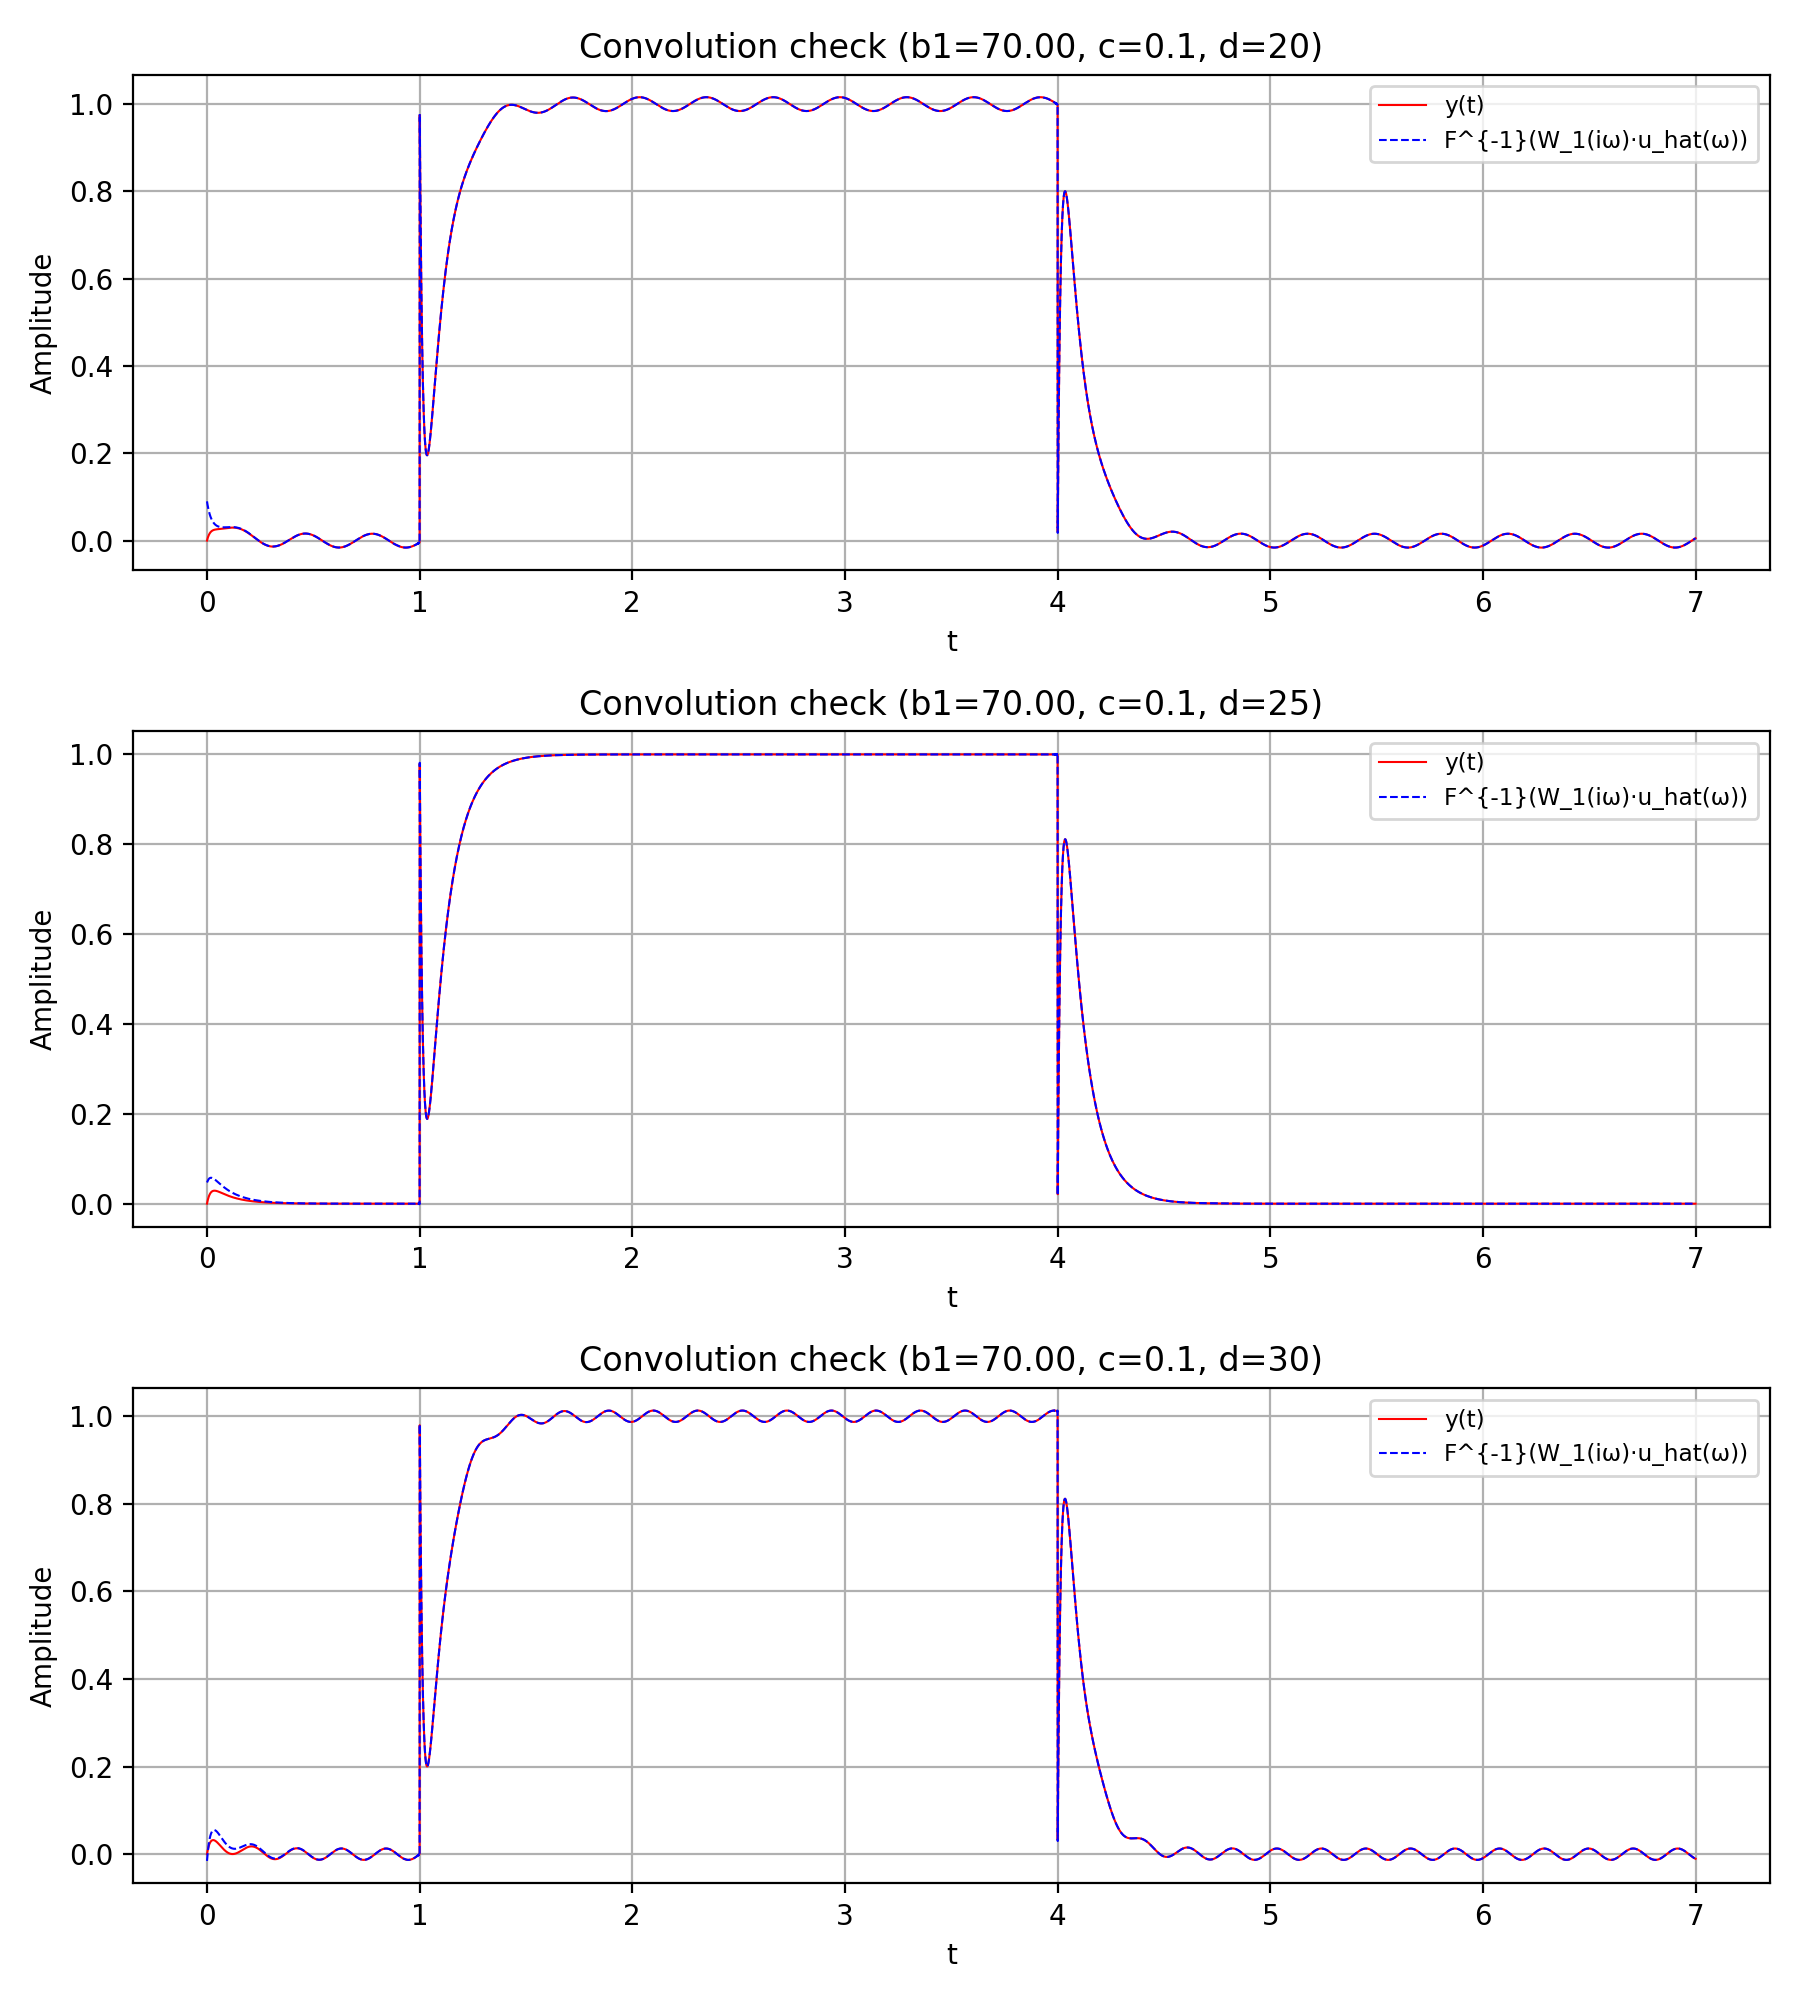
\includegraphics[width=1.0\linewidth]{fig/plots/Figure 33.png}
    \caption{Временная область}
    \label{fig:33}
\end{figure}
\begin{figure}[H]
    \centering
    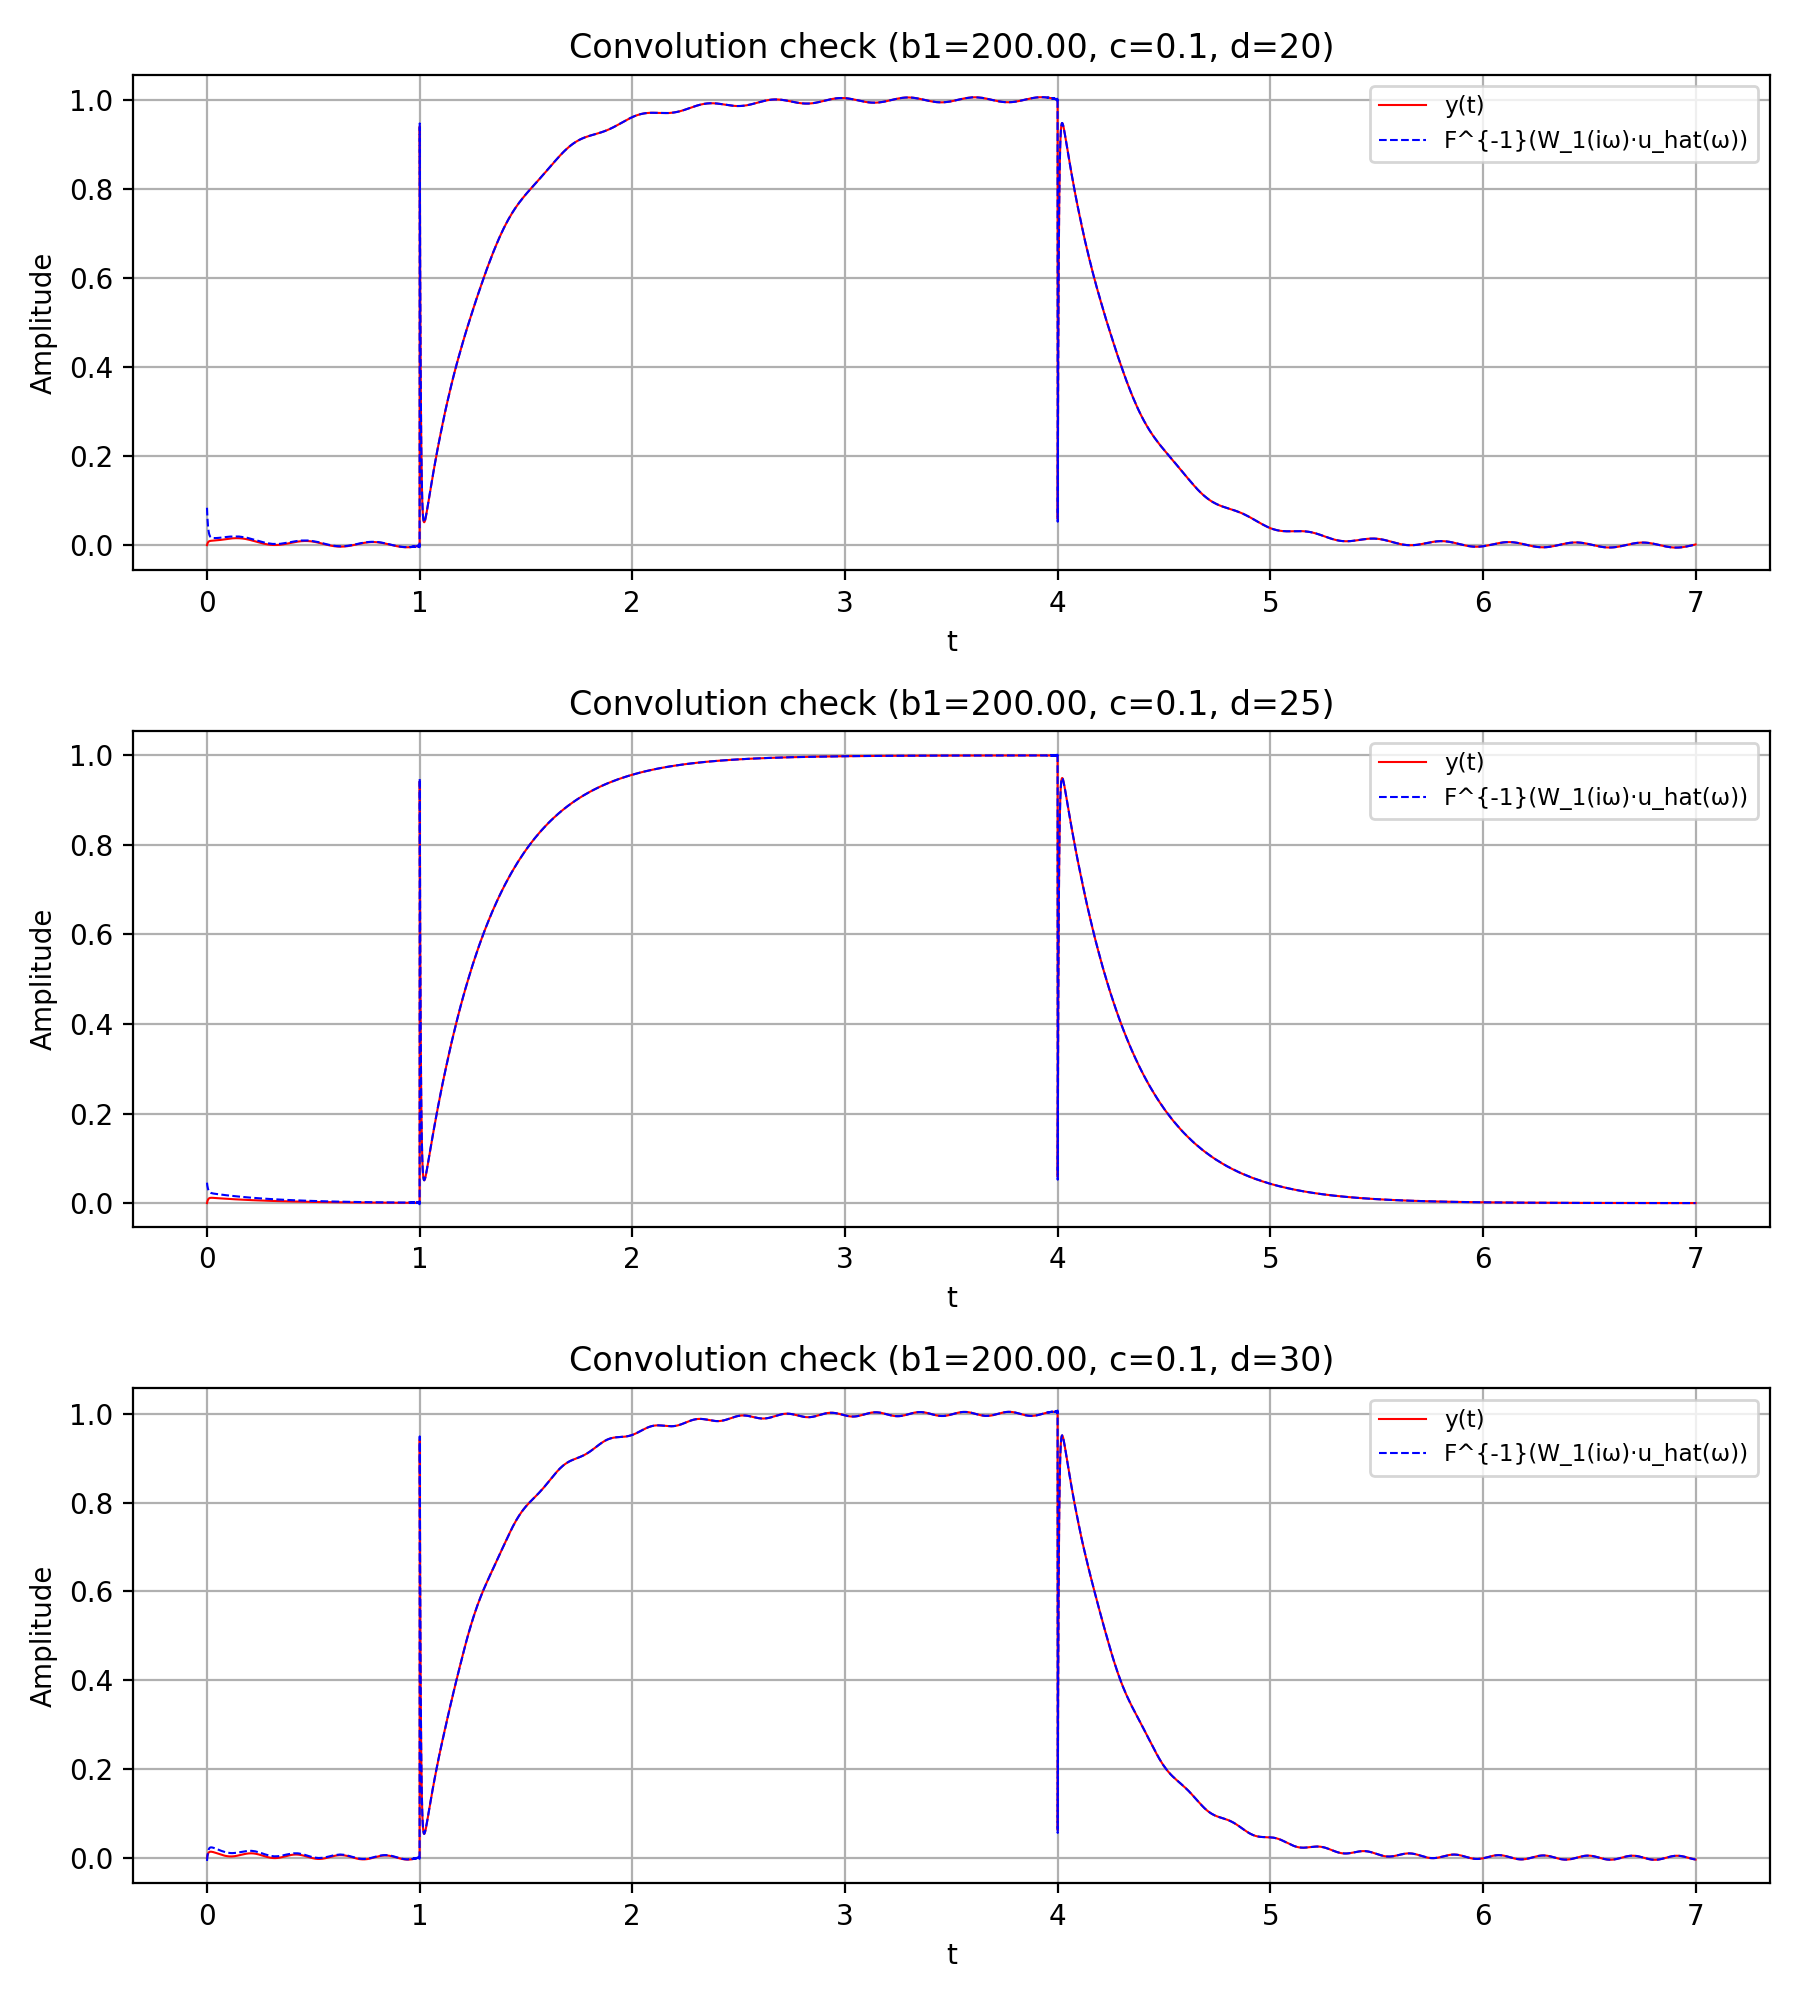
\includegraphics[width=1.0\linewidth]{fig/plots/Figure 34.png}
    \caption{Временная область}
    \label{fig:34}
\end{figure}
\begin{figure}[H]
    \centering
    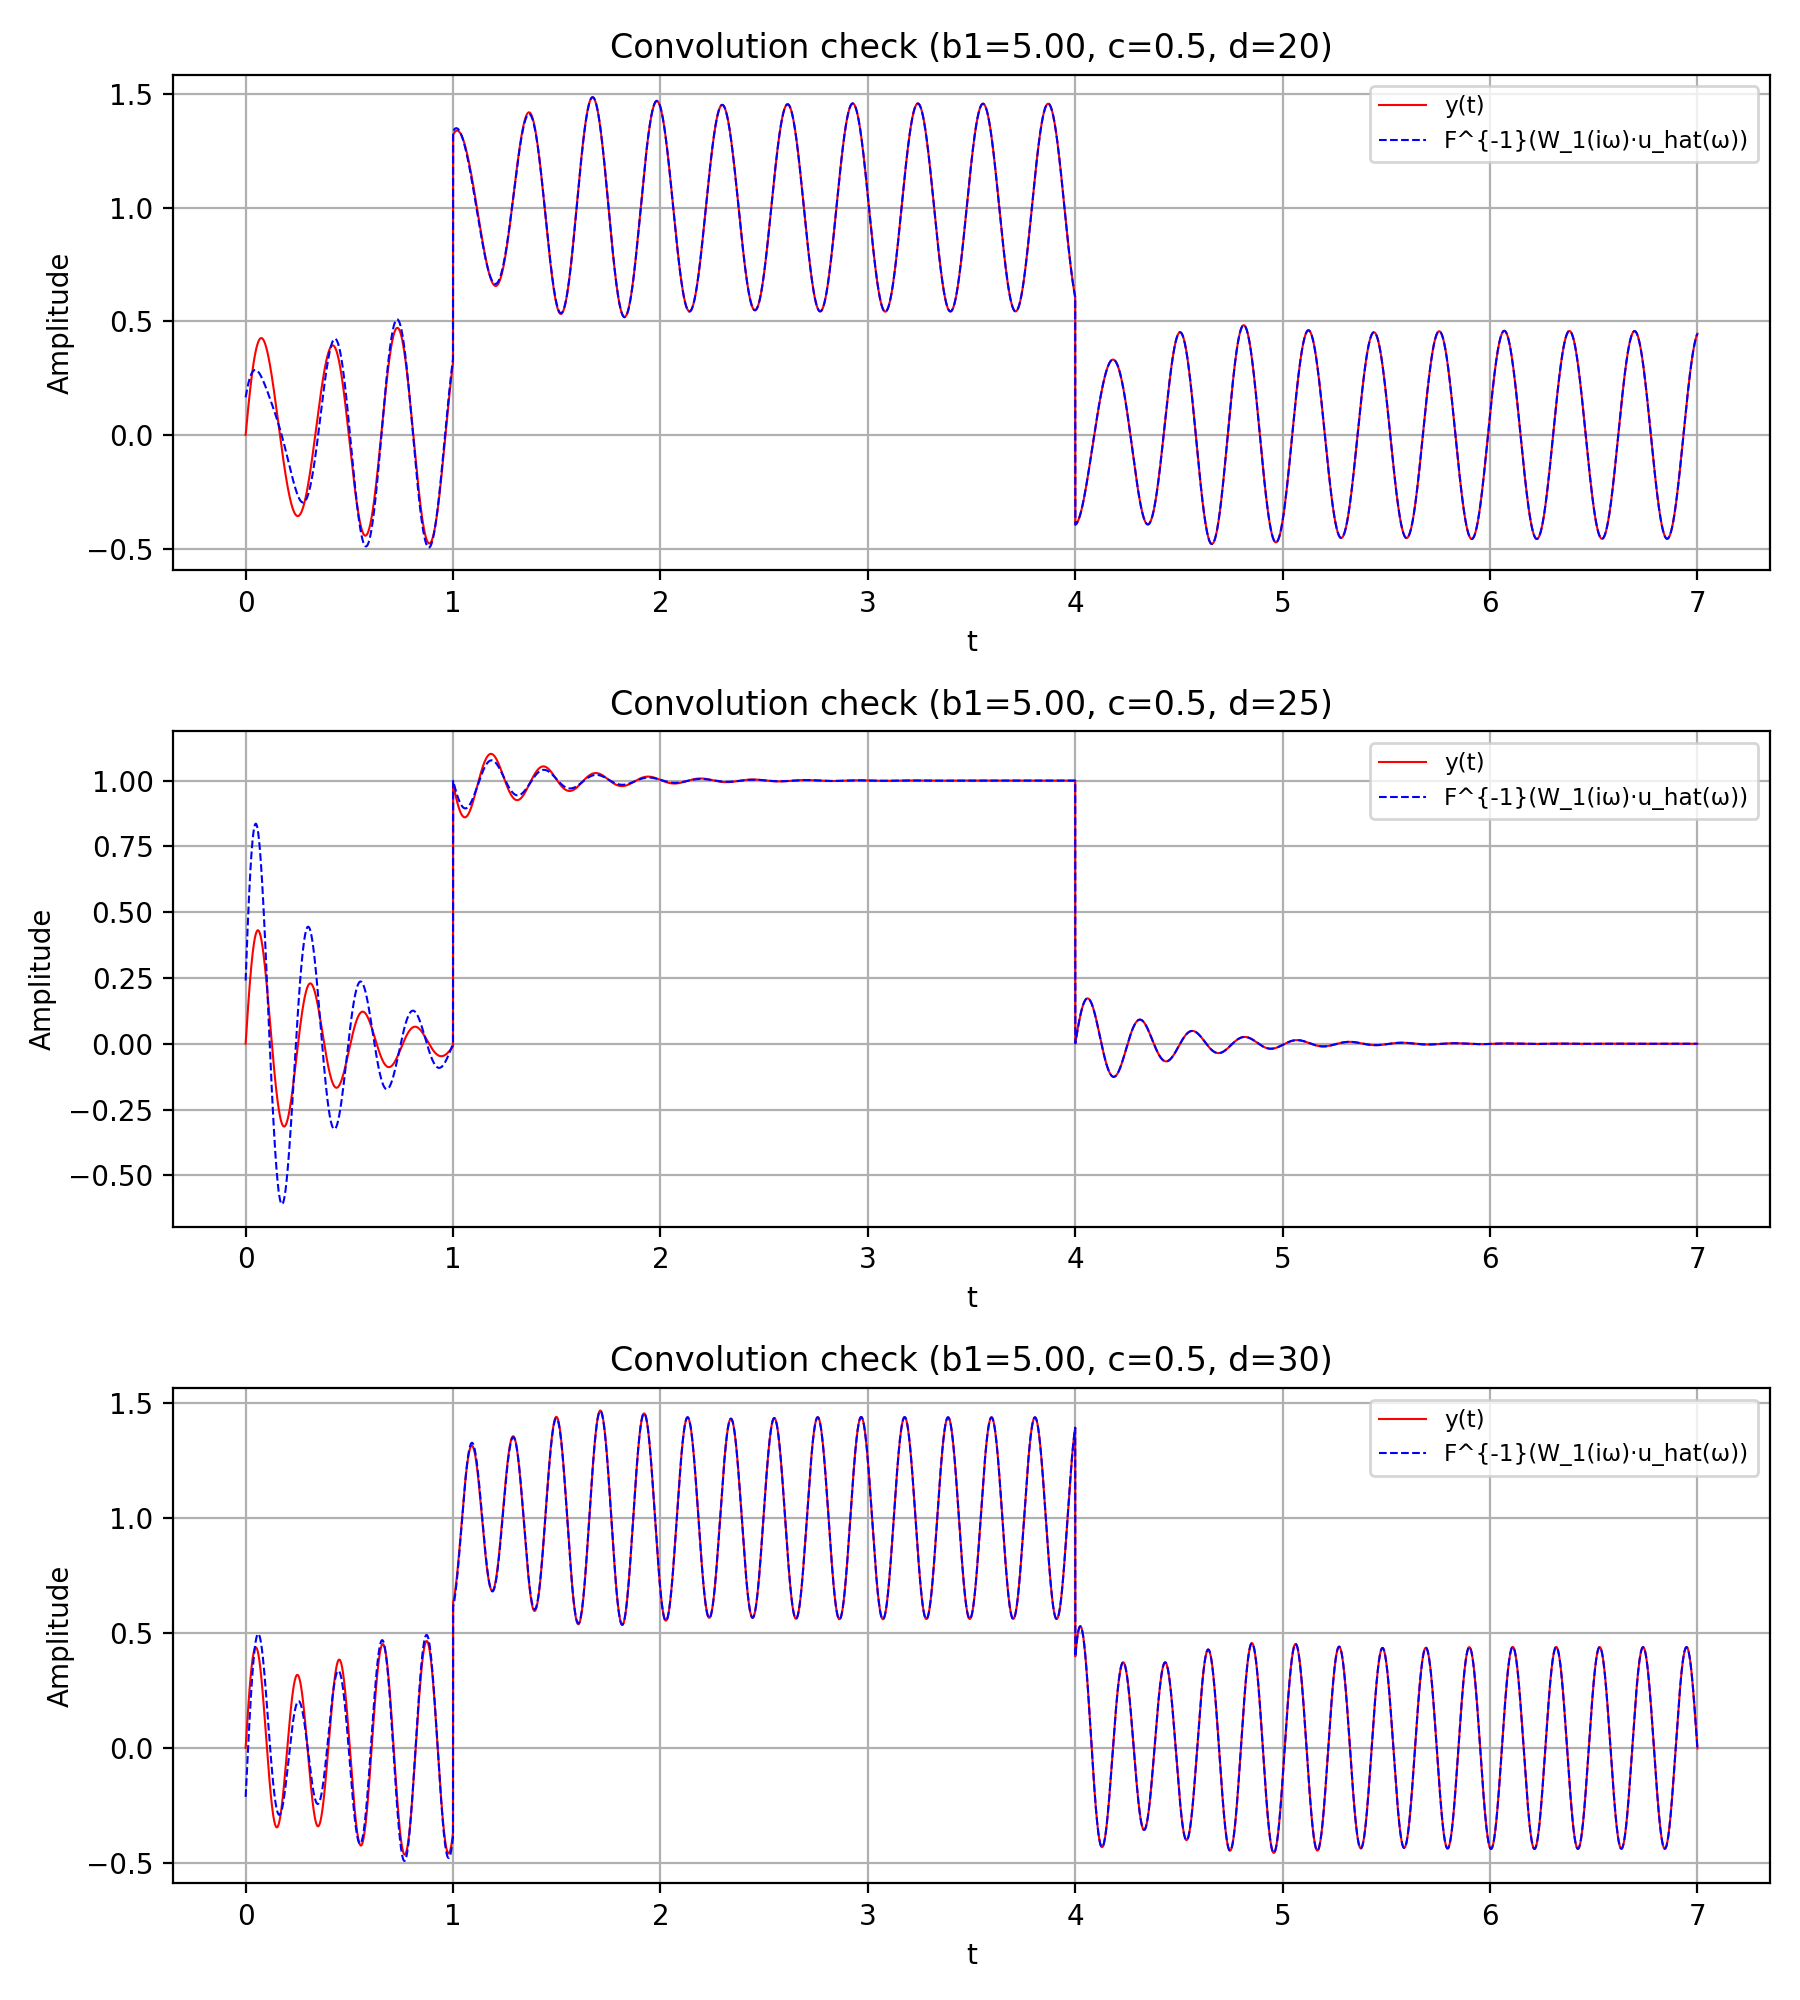
\includegraphics[width=1.0\linewidth]{fig/plots/Figure 35.png}
    \caption{Временная область}
    \label{fig:35}
\end{figure}
\begin{figure}[H]
    \centering
    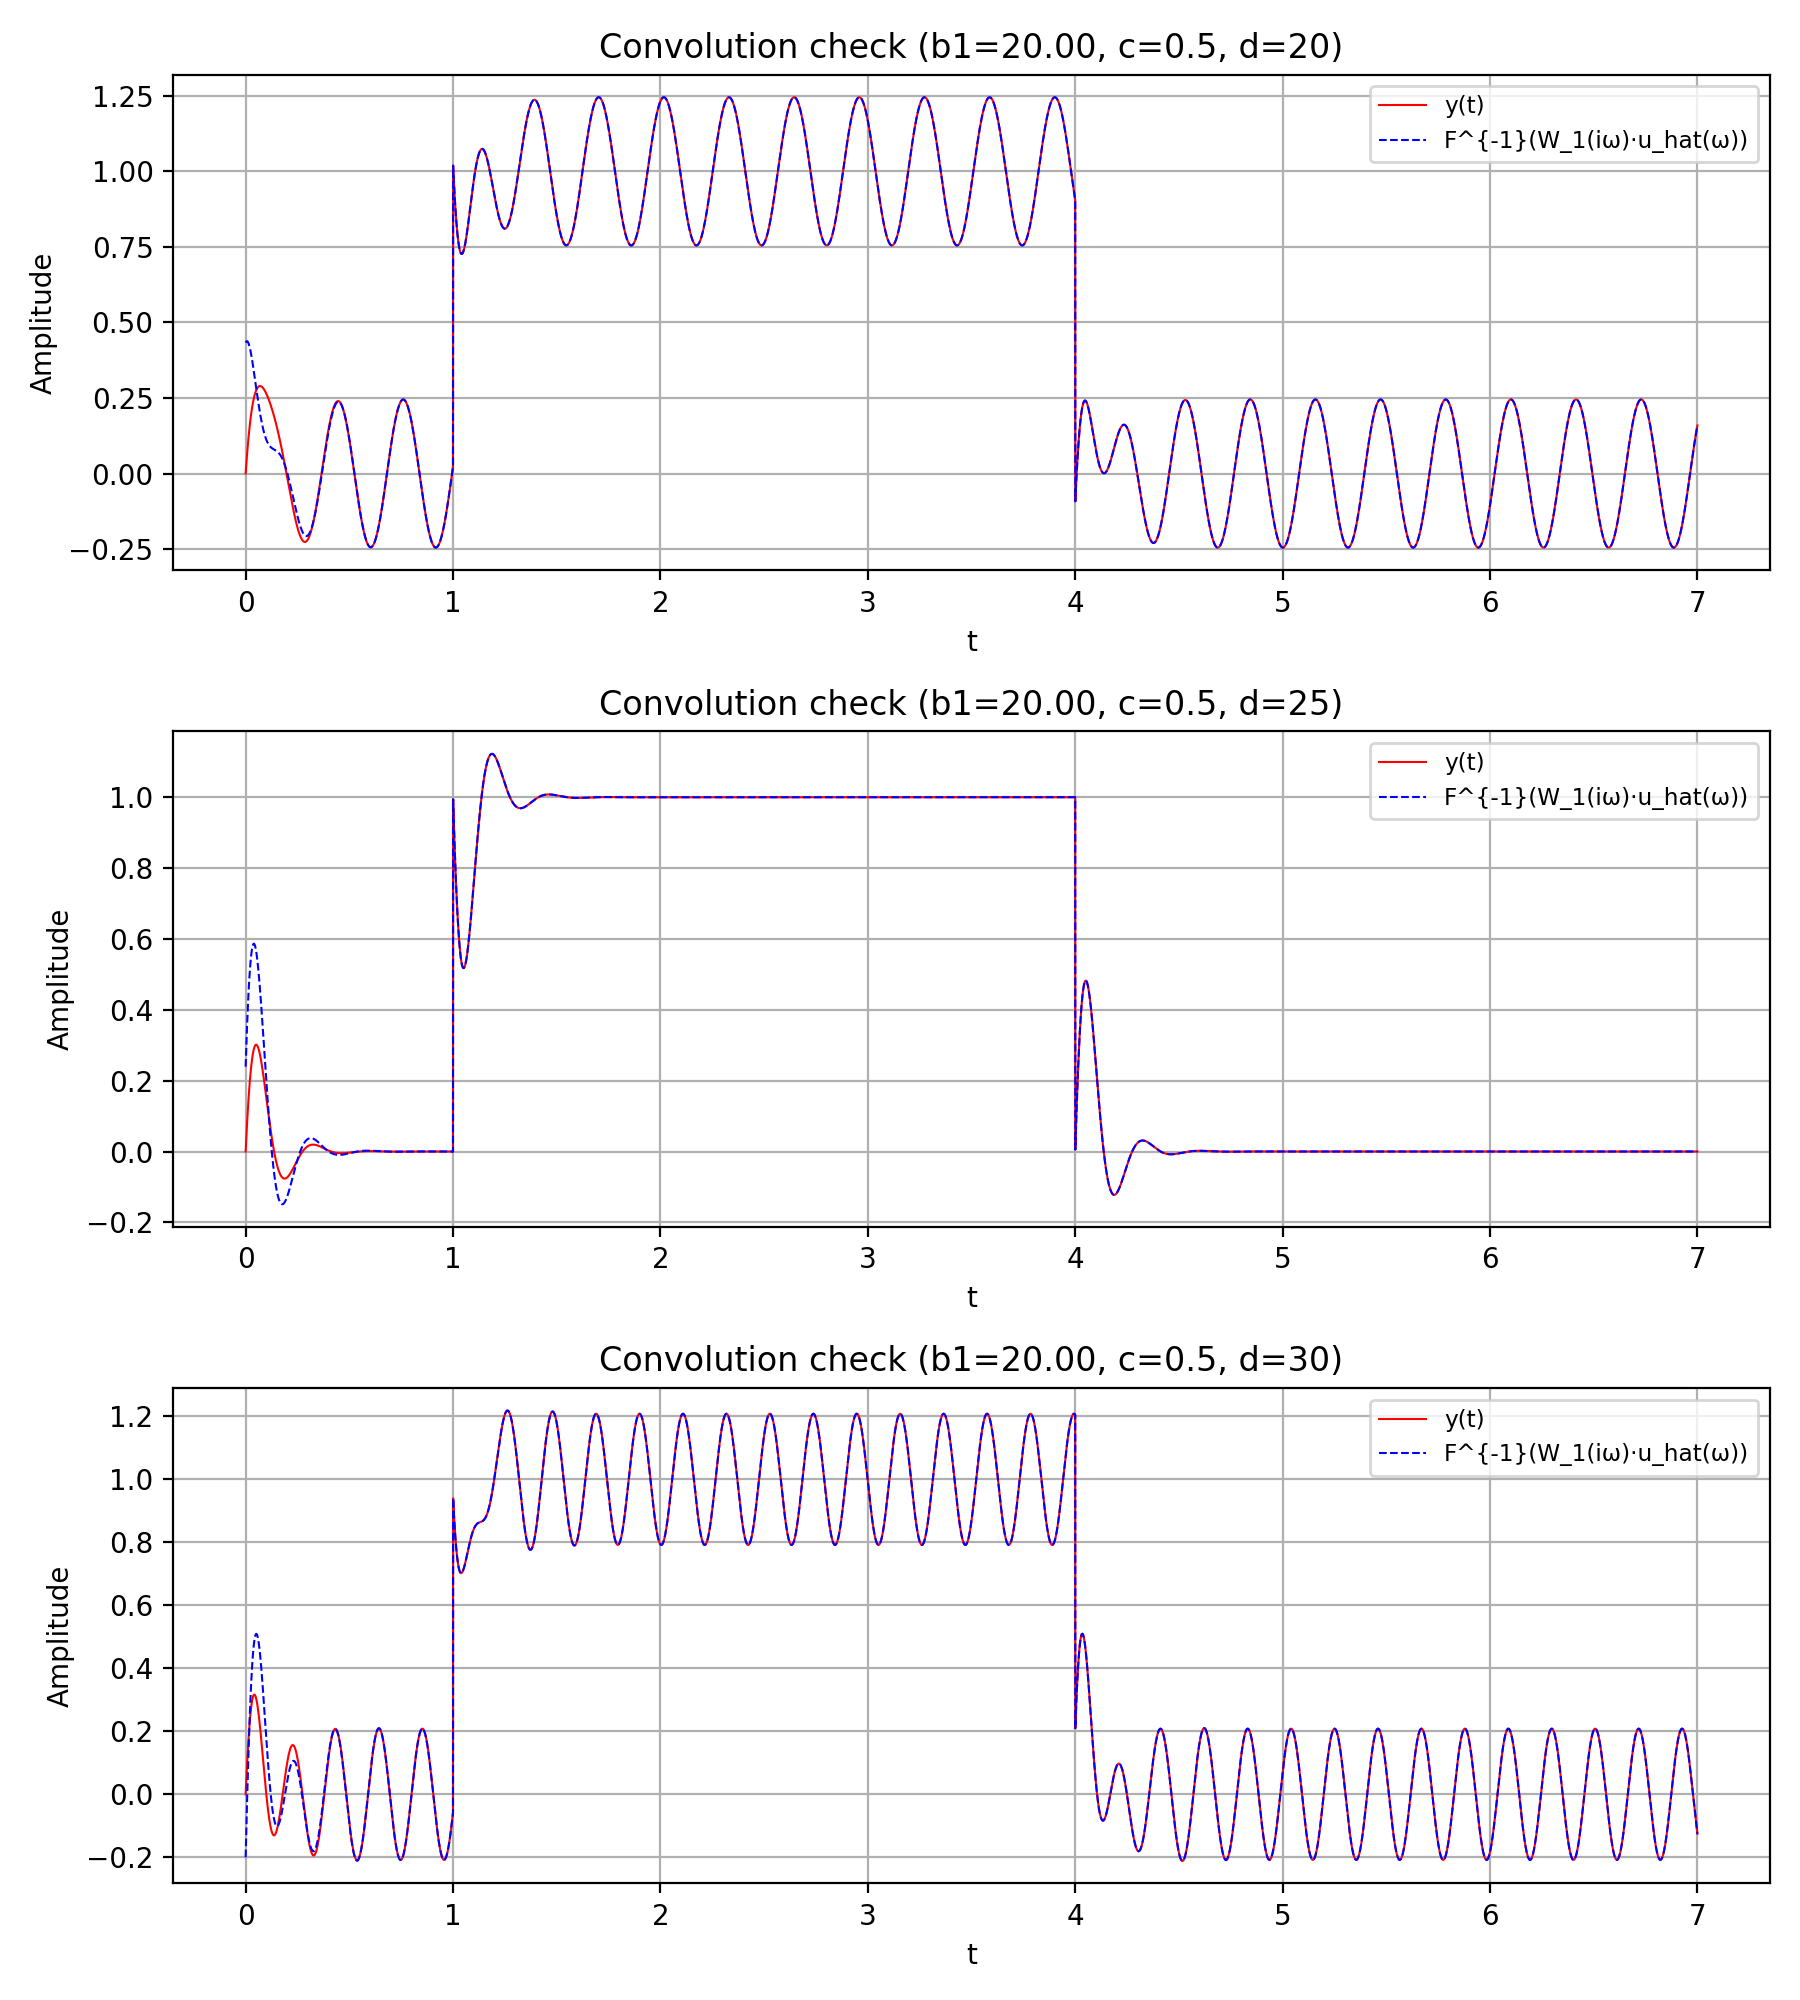
\includegraphics[width=1.0\linewidth]{fig/plots/Figure 36.png}
    \caption{Временная область}
    \label{fig:36}
\end{figure}
\begin{figure}[H]
    \centering
    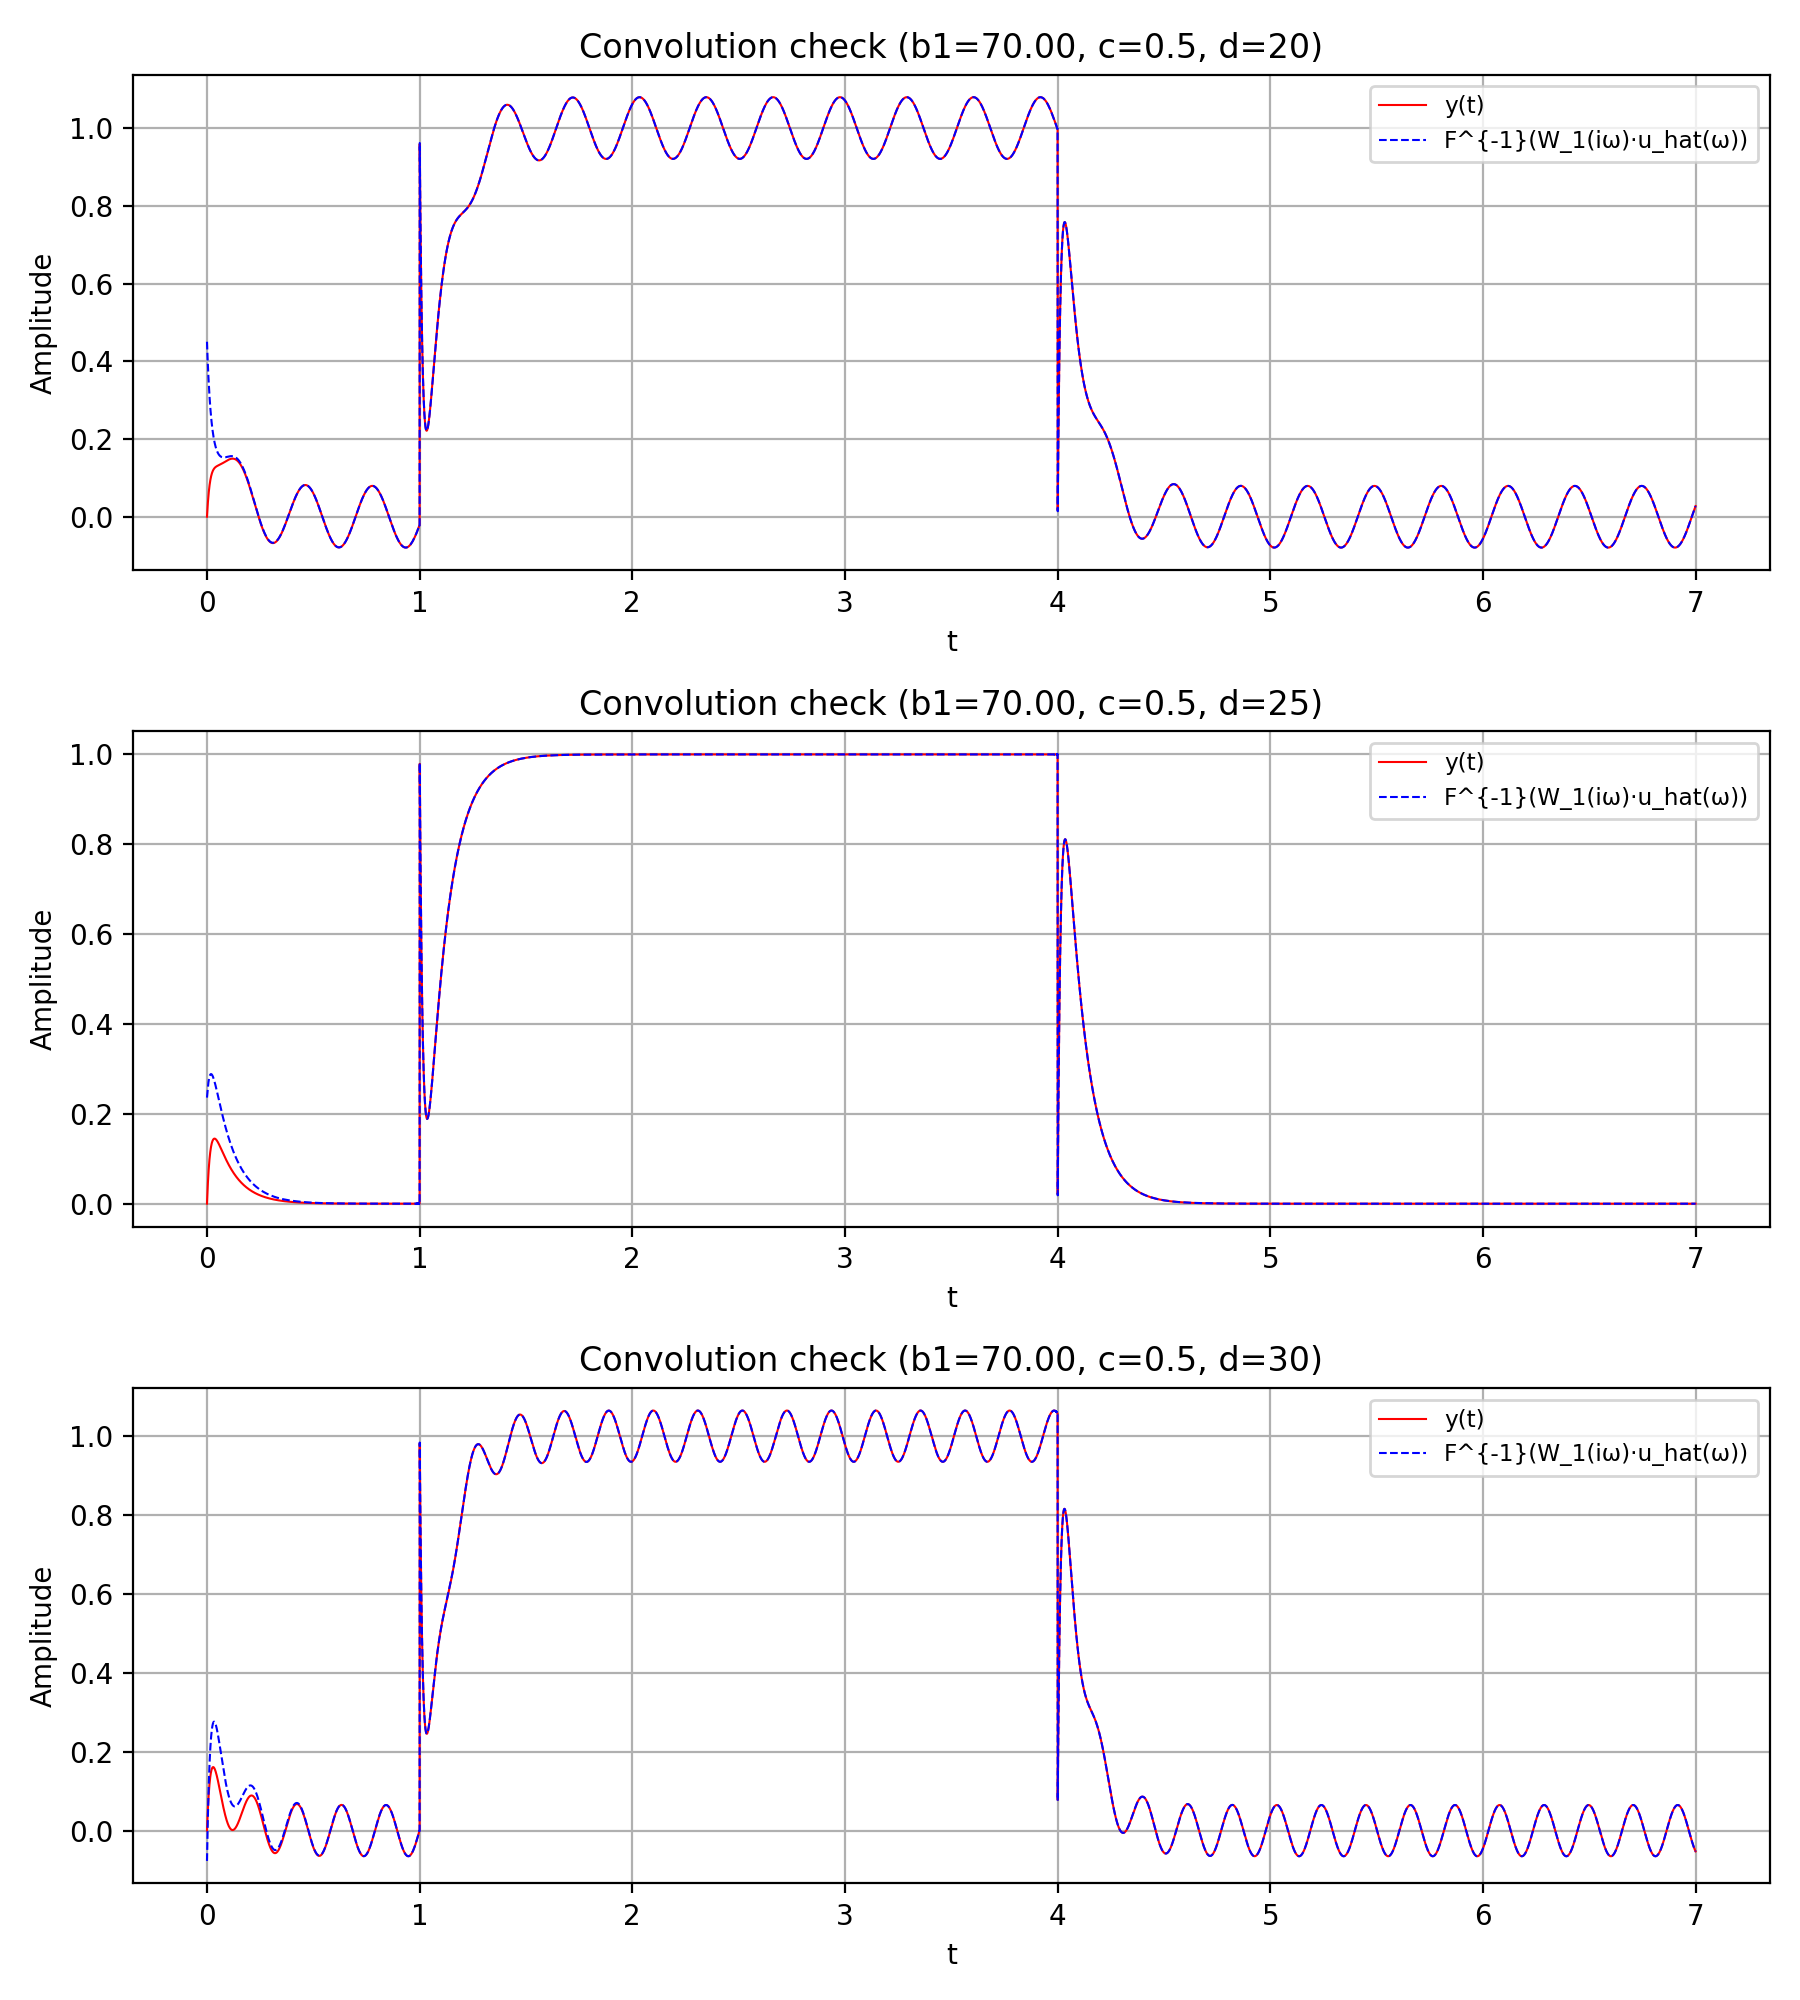
\includegraphics[width=1.0\linewidth]{fig/plots/Figure 37.png}
    \caption{Временная область}
    \label{fig:37}
\end{figure}
\begin{figure}[H]
    \centering
    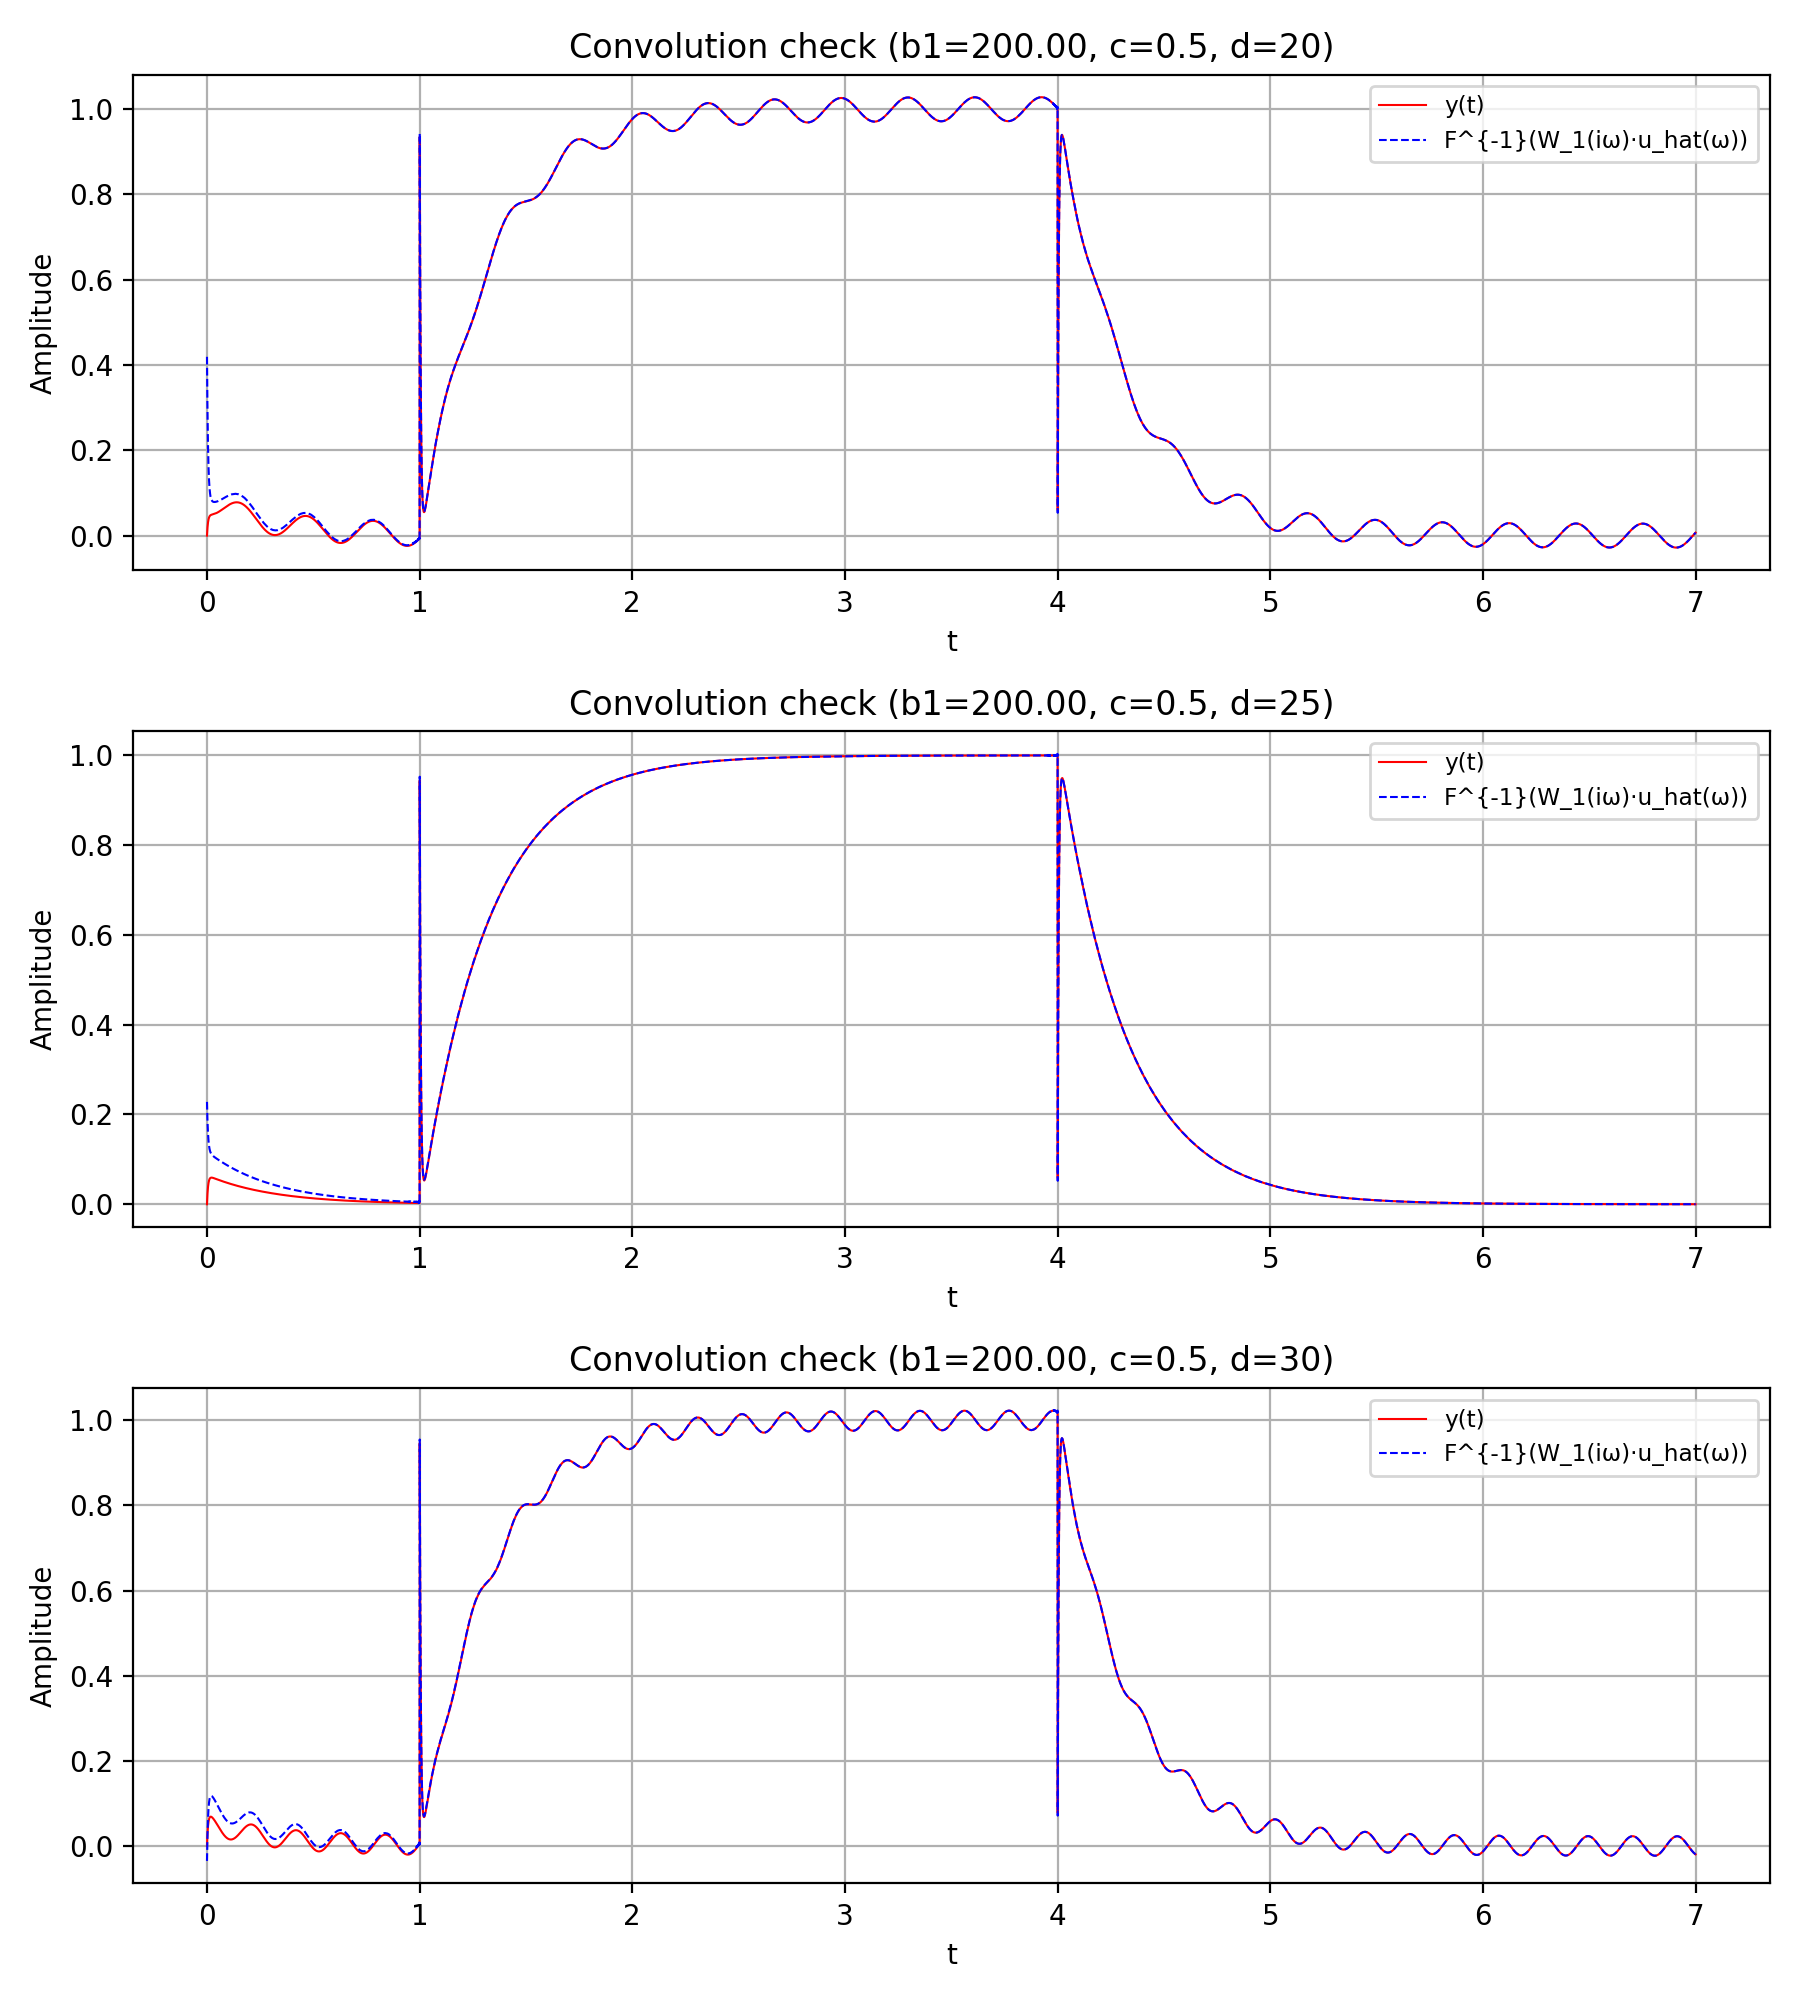
\includegraphics[width=1.0\linewidth]{fig/plots/Figure 38.png}
    \caption{Временная область}
    \label{fig:38}
\end{figure}

\begin{figure}[H]
    \centering
    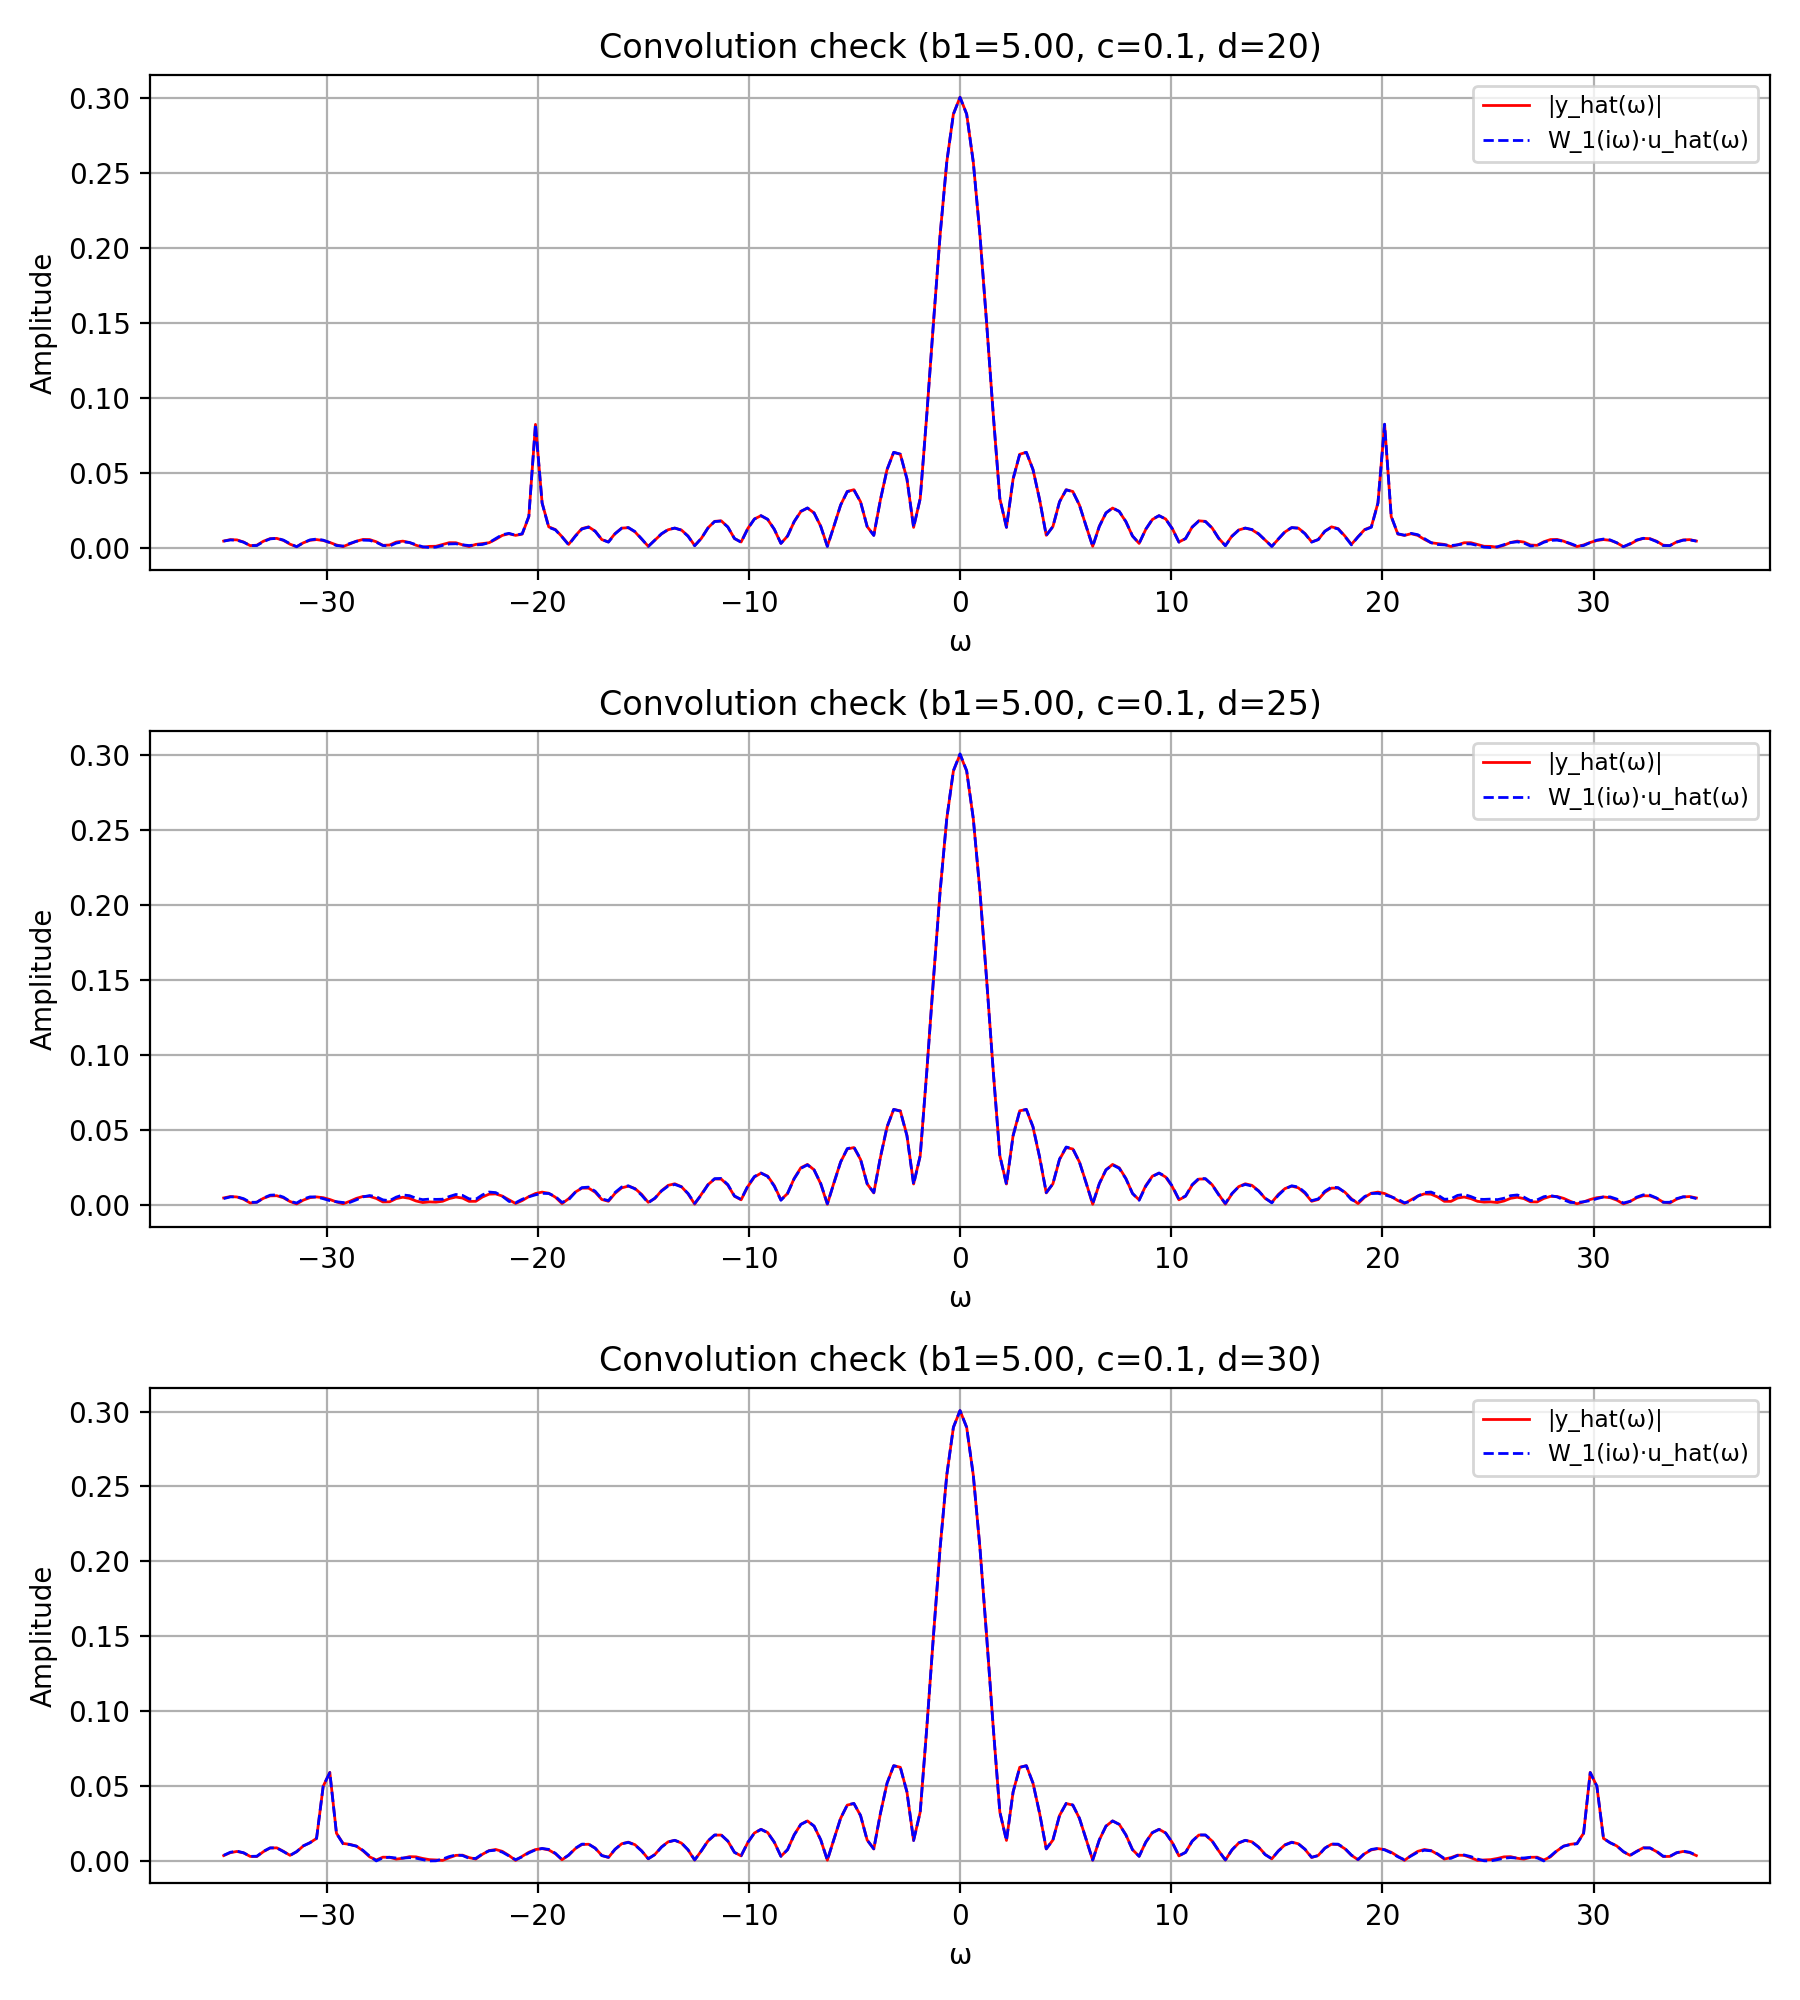
\includegraphics[width=1.0\linewidth]{fig/plots/Figure 39.png}
    \caption{Частотная область}
    \label{fig:39}
\end{figure}
\begin{figure}[H]
    \centering
    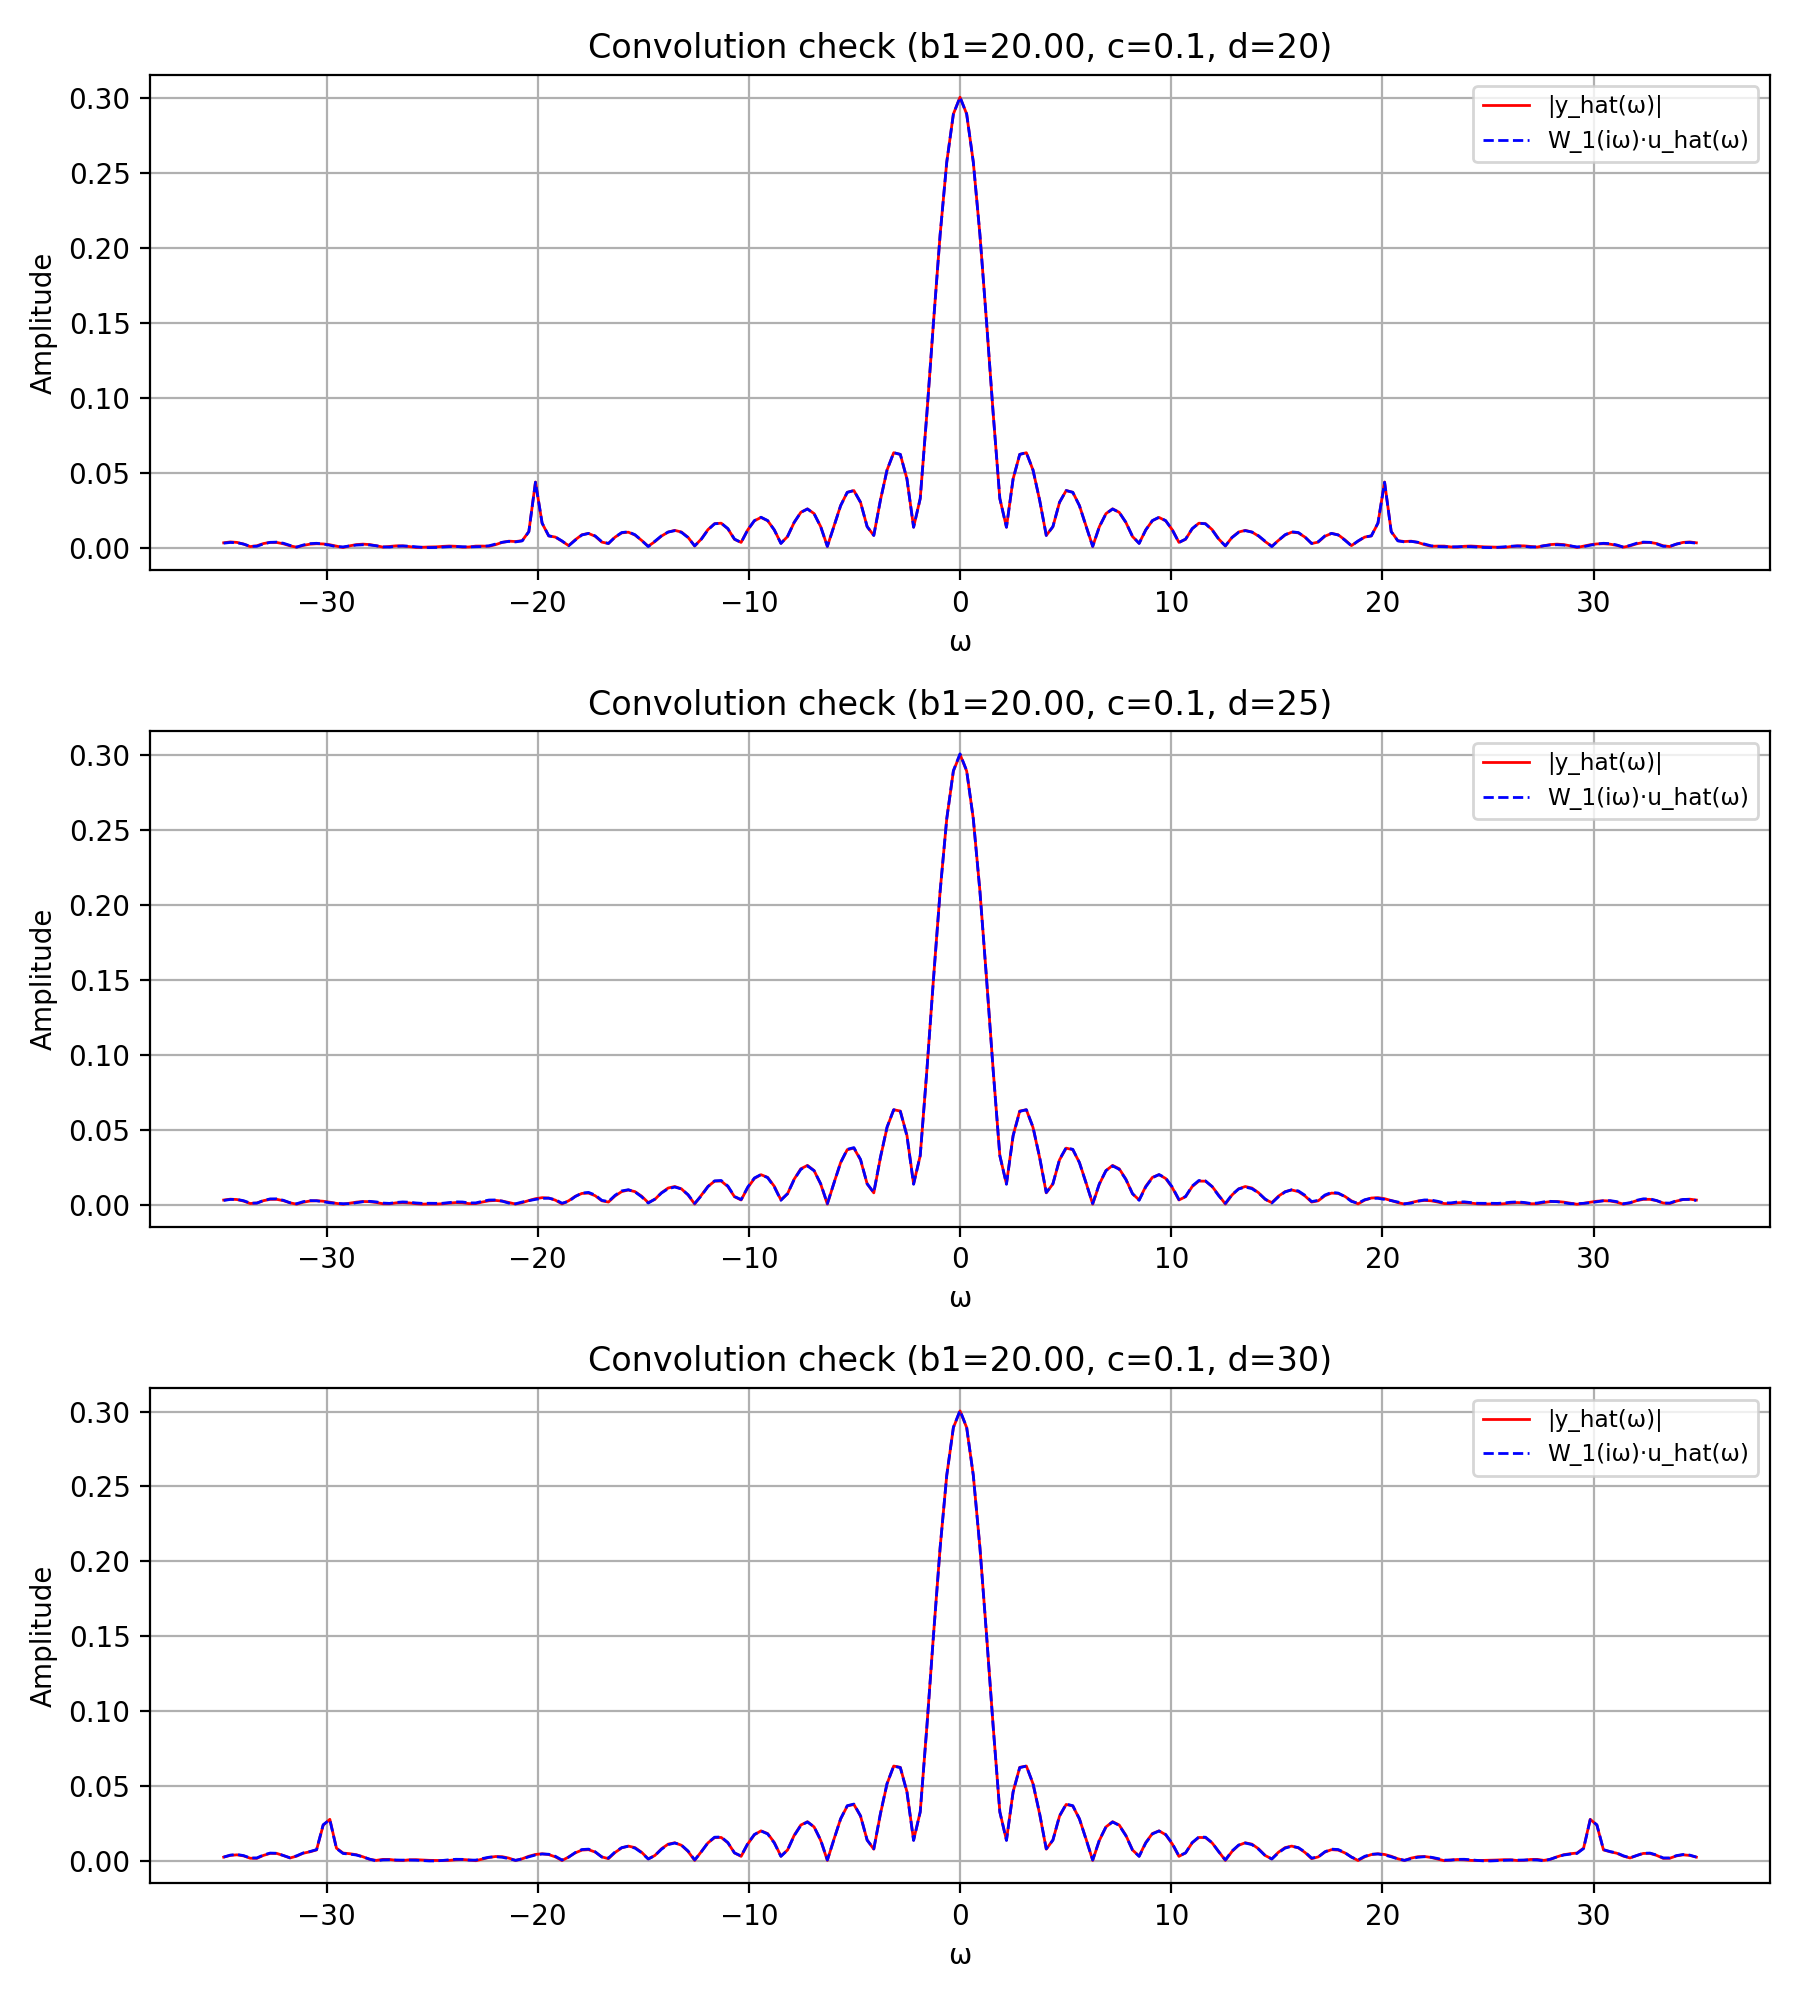
\includegraphics[width=1.0\linewidth]{fig/plots/Figure 40.png}
    \caption{Частотная область}
    \label{fig:40}
\end{figure}
\begin{figure}[H]
    \centering
    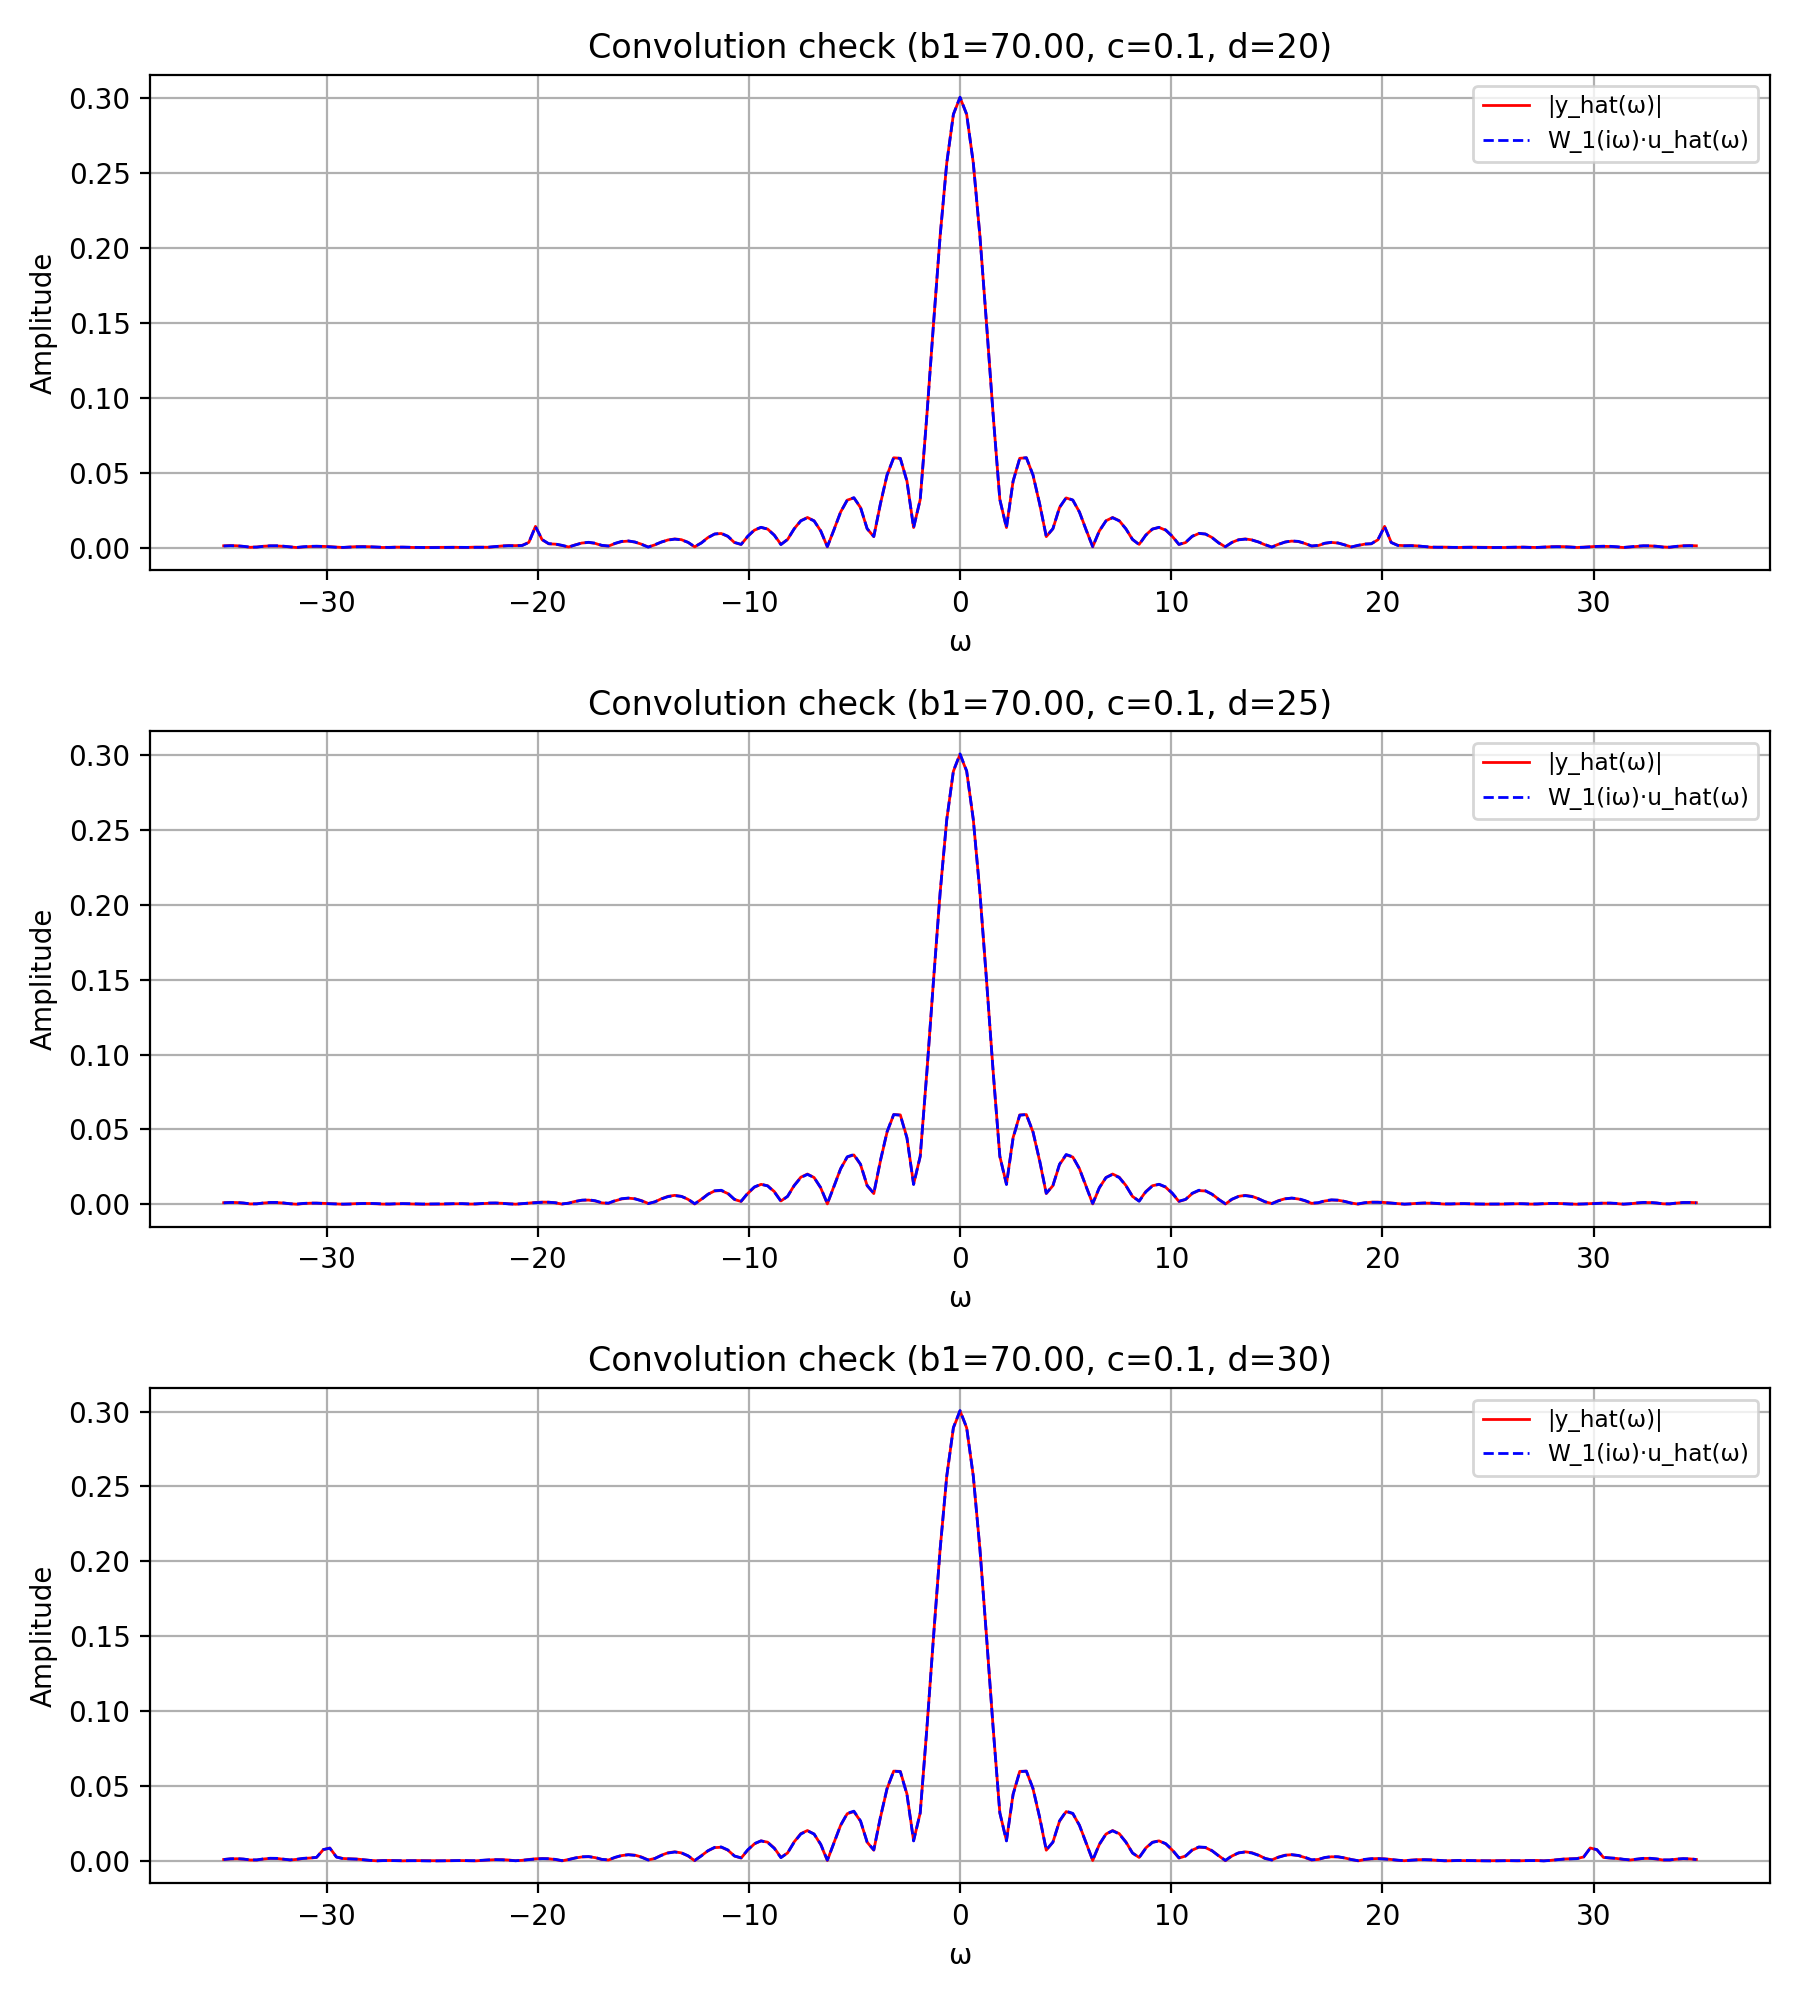
\includegraphics[width=1.0\linewidth]{fig/plots/Figure 41.png}
    \caption{Частотная область}
    \label{fig:41}
\end{figure}
\begin{figure}[H]
    \centering
    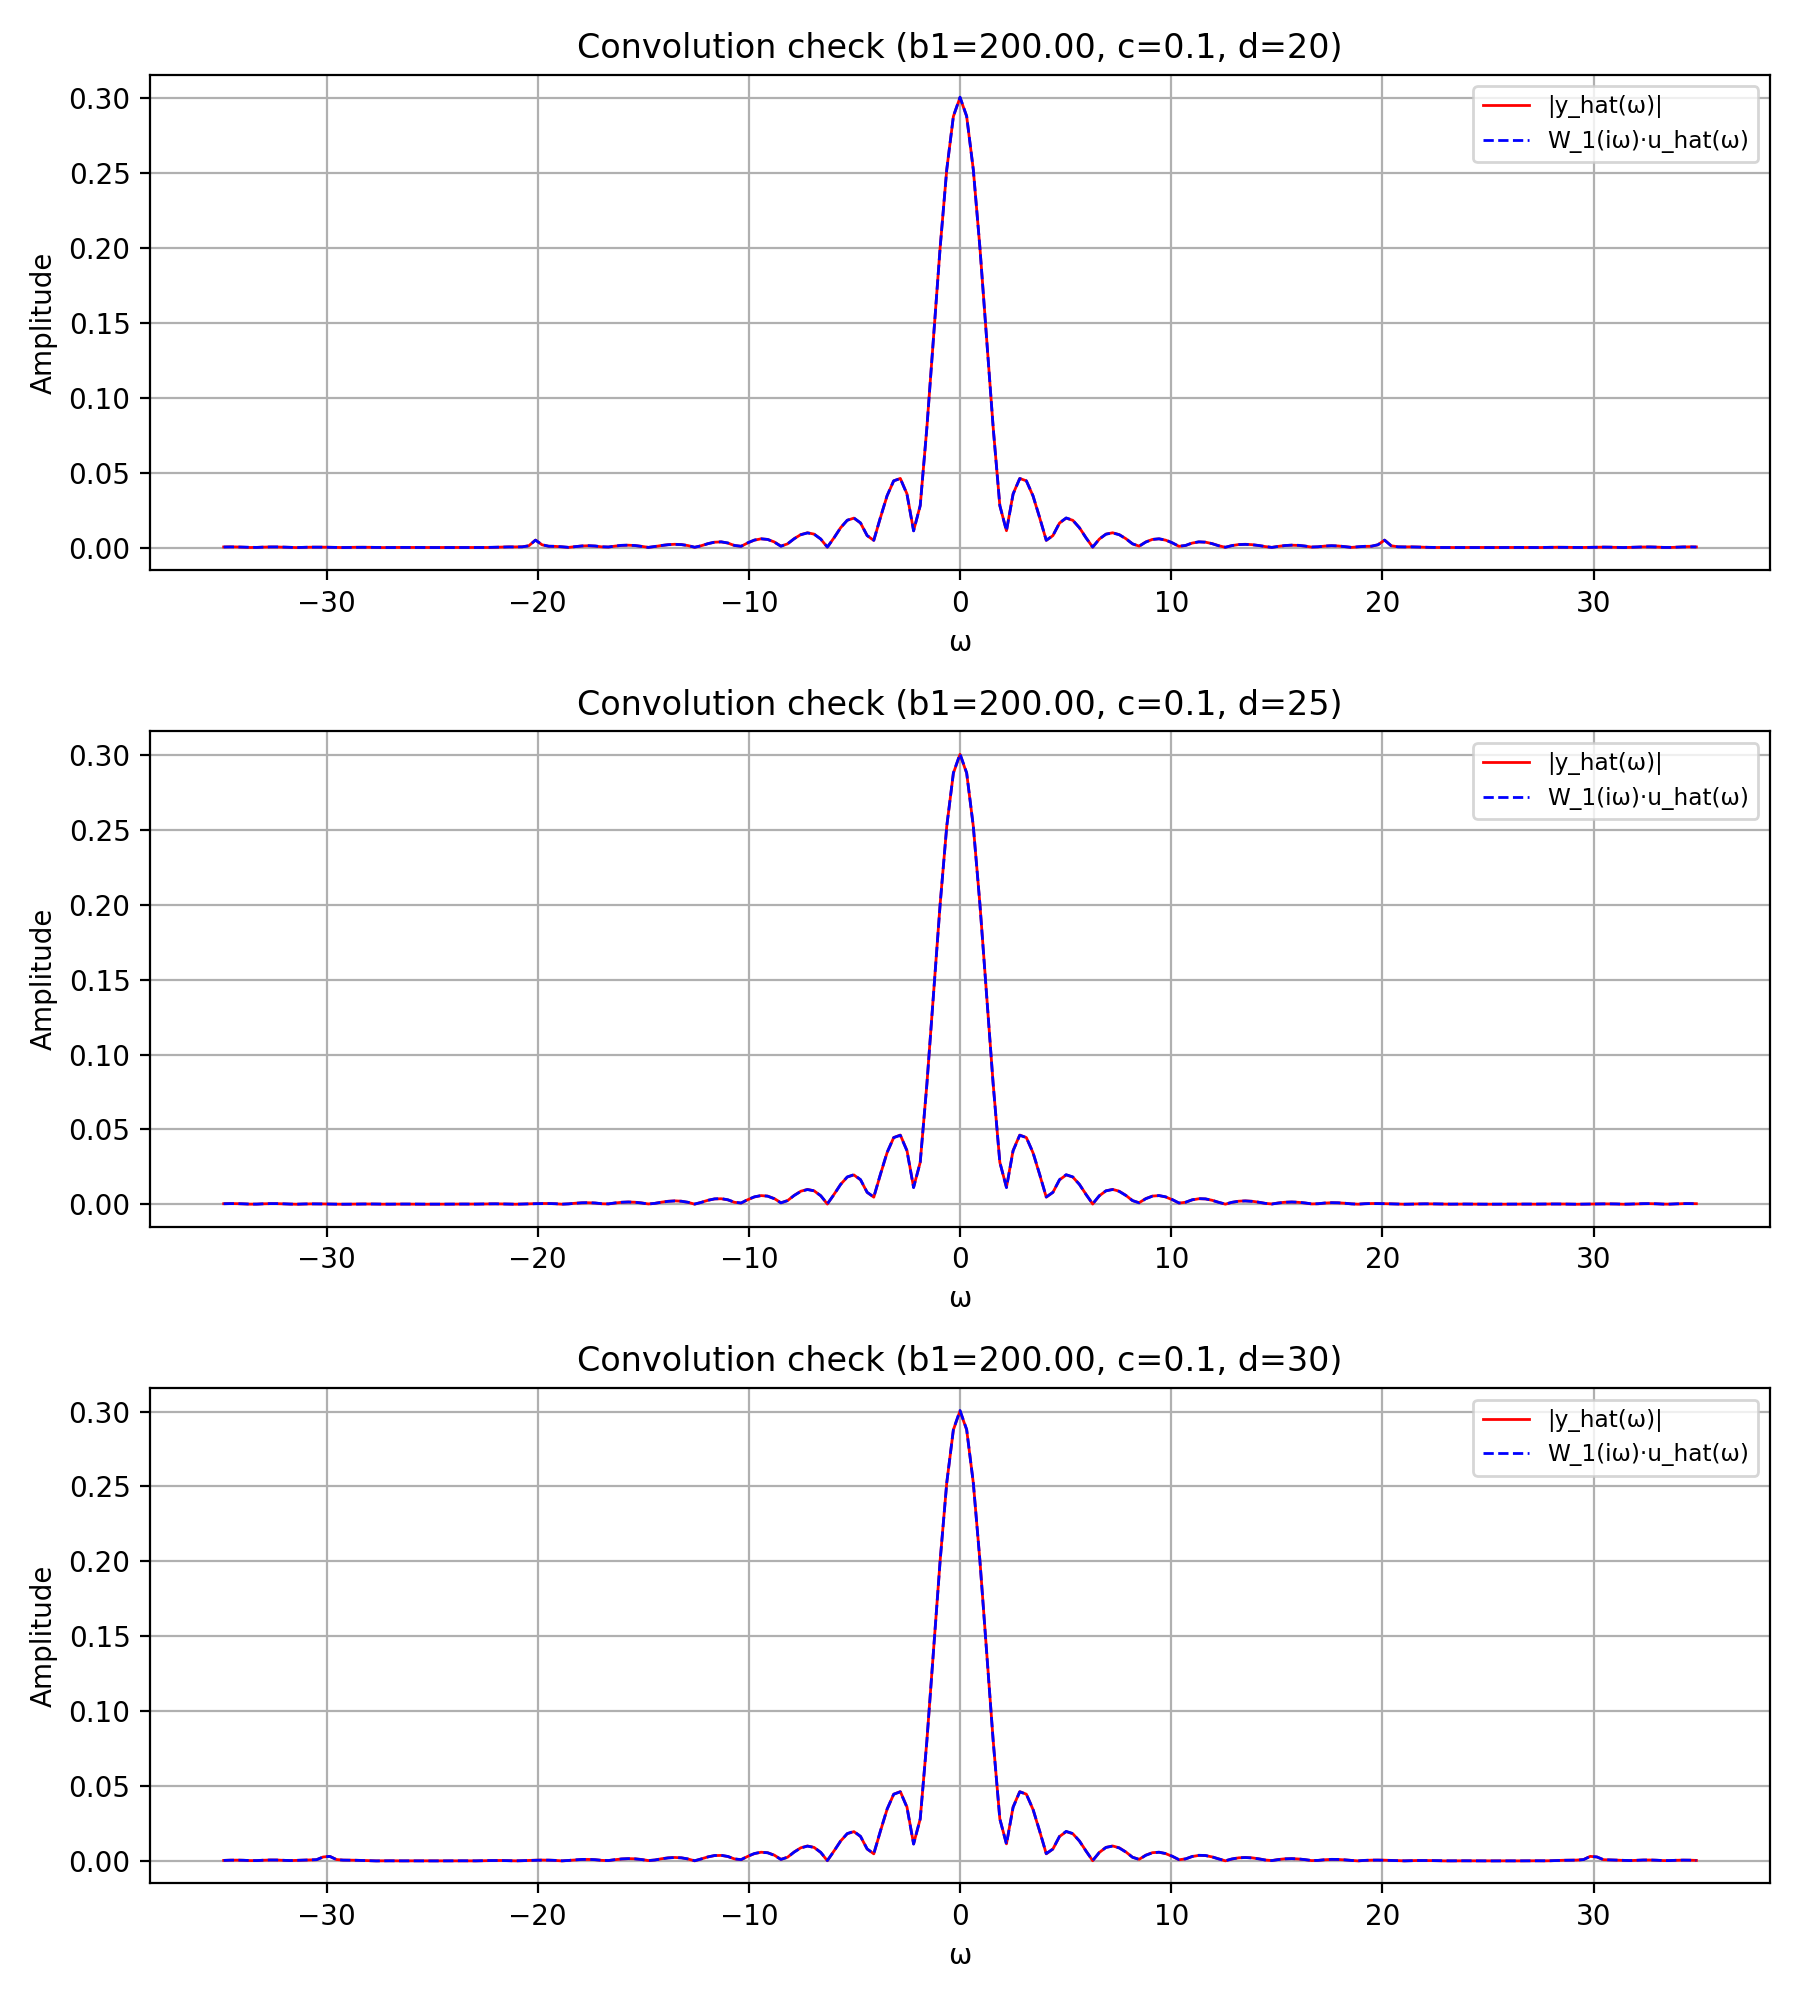
\includegraphics[width=1.0\linewidth]{fig/plots/Figure 42.png}
    \caption{Частотная область}
    \label{fig:42}
\end{figure}
\begin{figure}[H]
    \centering
    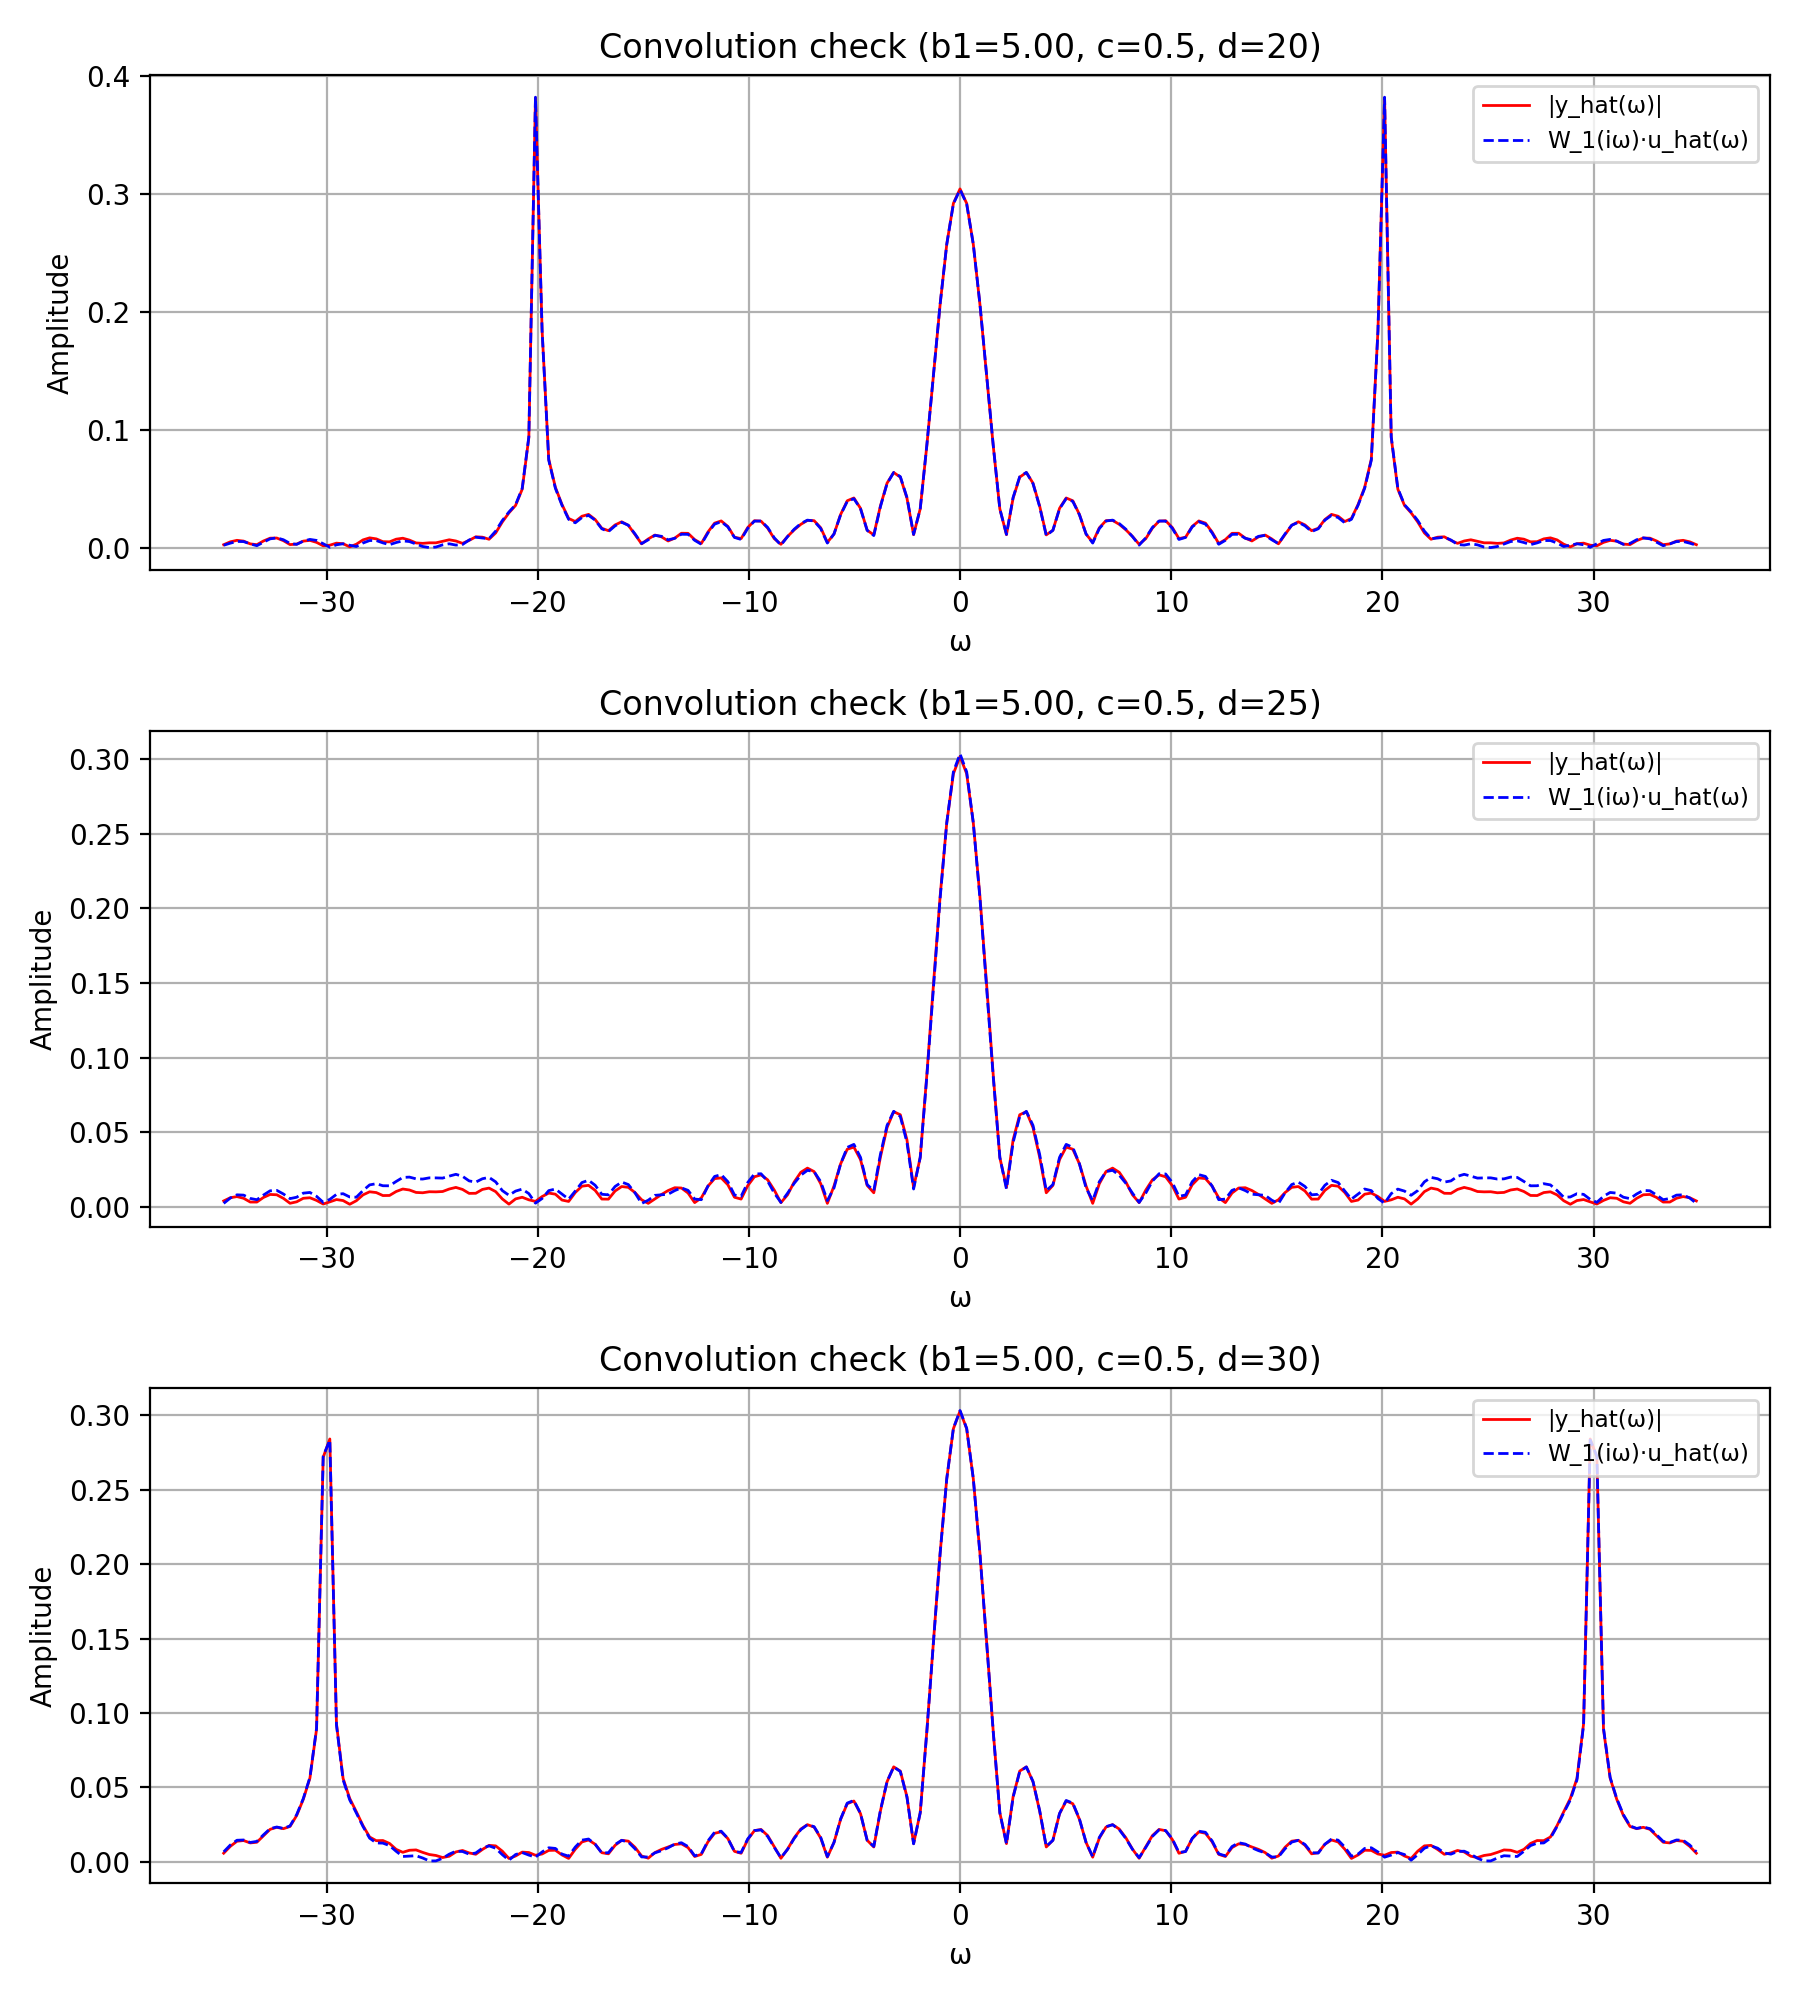
\includegraphics[width=1.0\linewidth]{fig/plots/Figure 43.png}
    \caption{Частотная область}
    \label{fig:43}
\end{figure}
\begin{figure}[H]
    \centering
    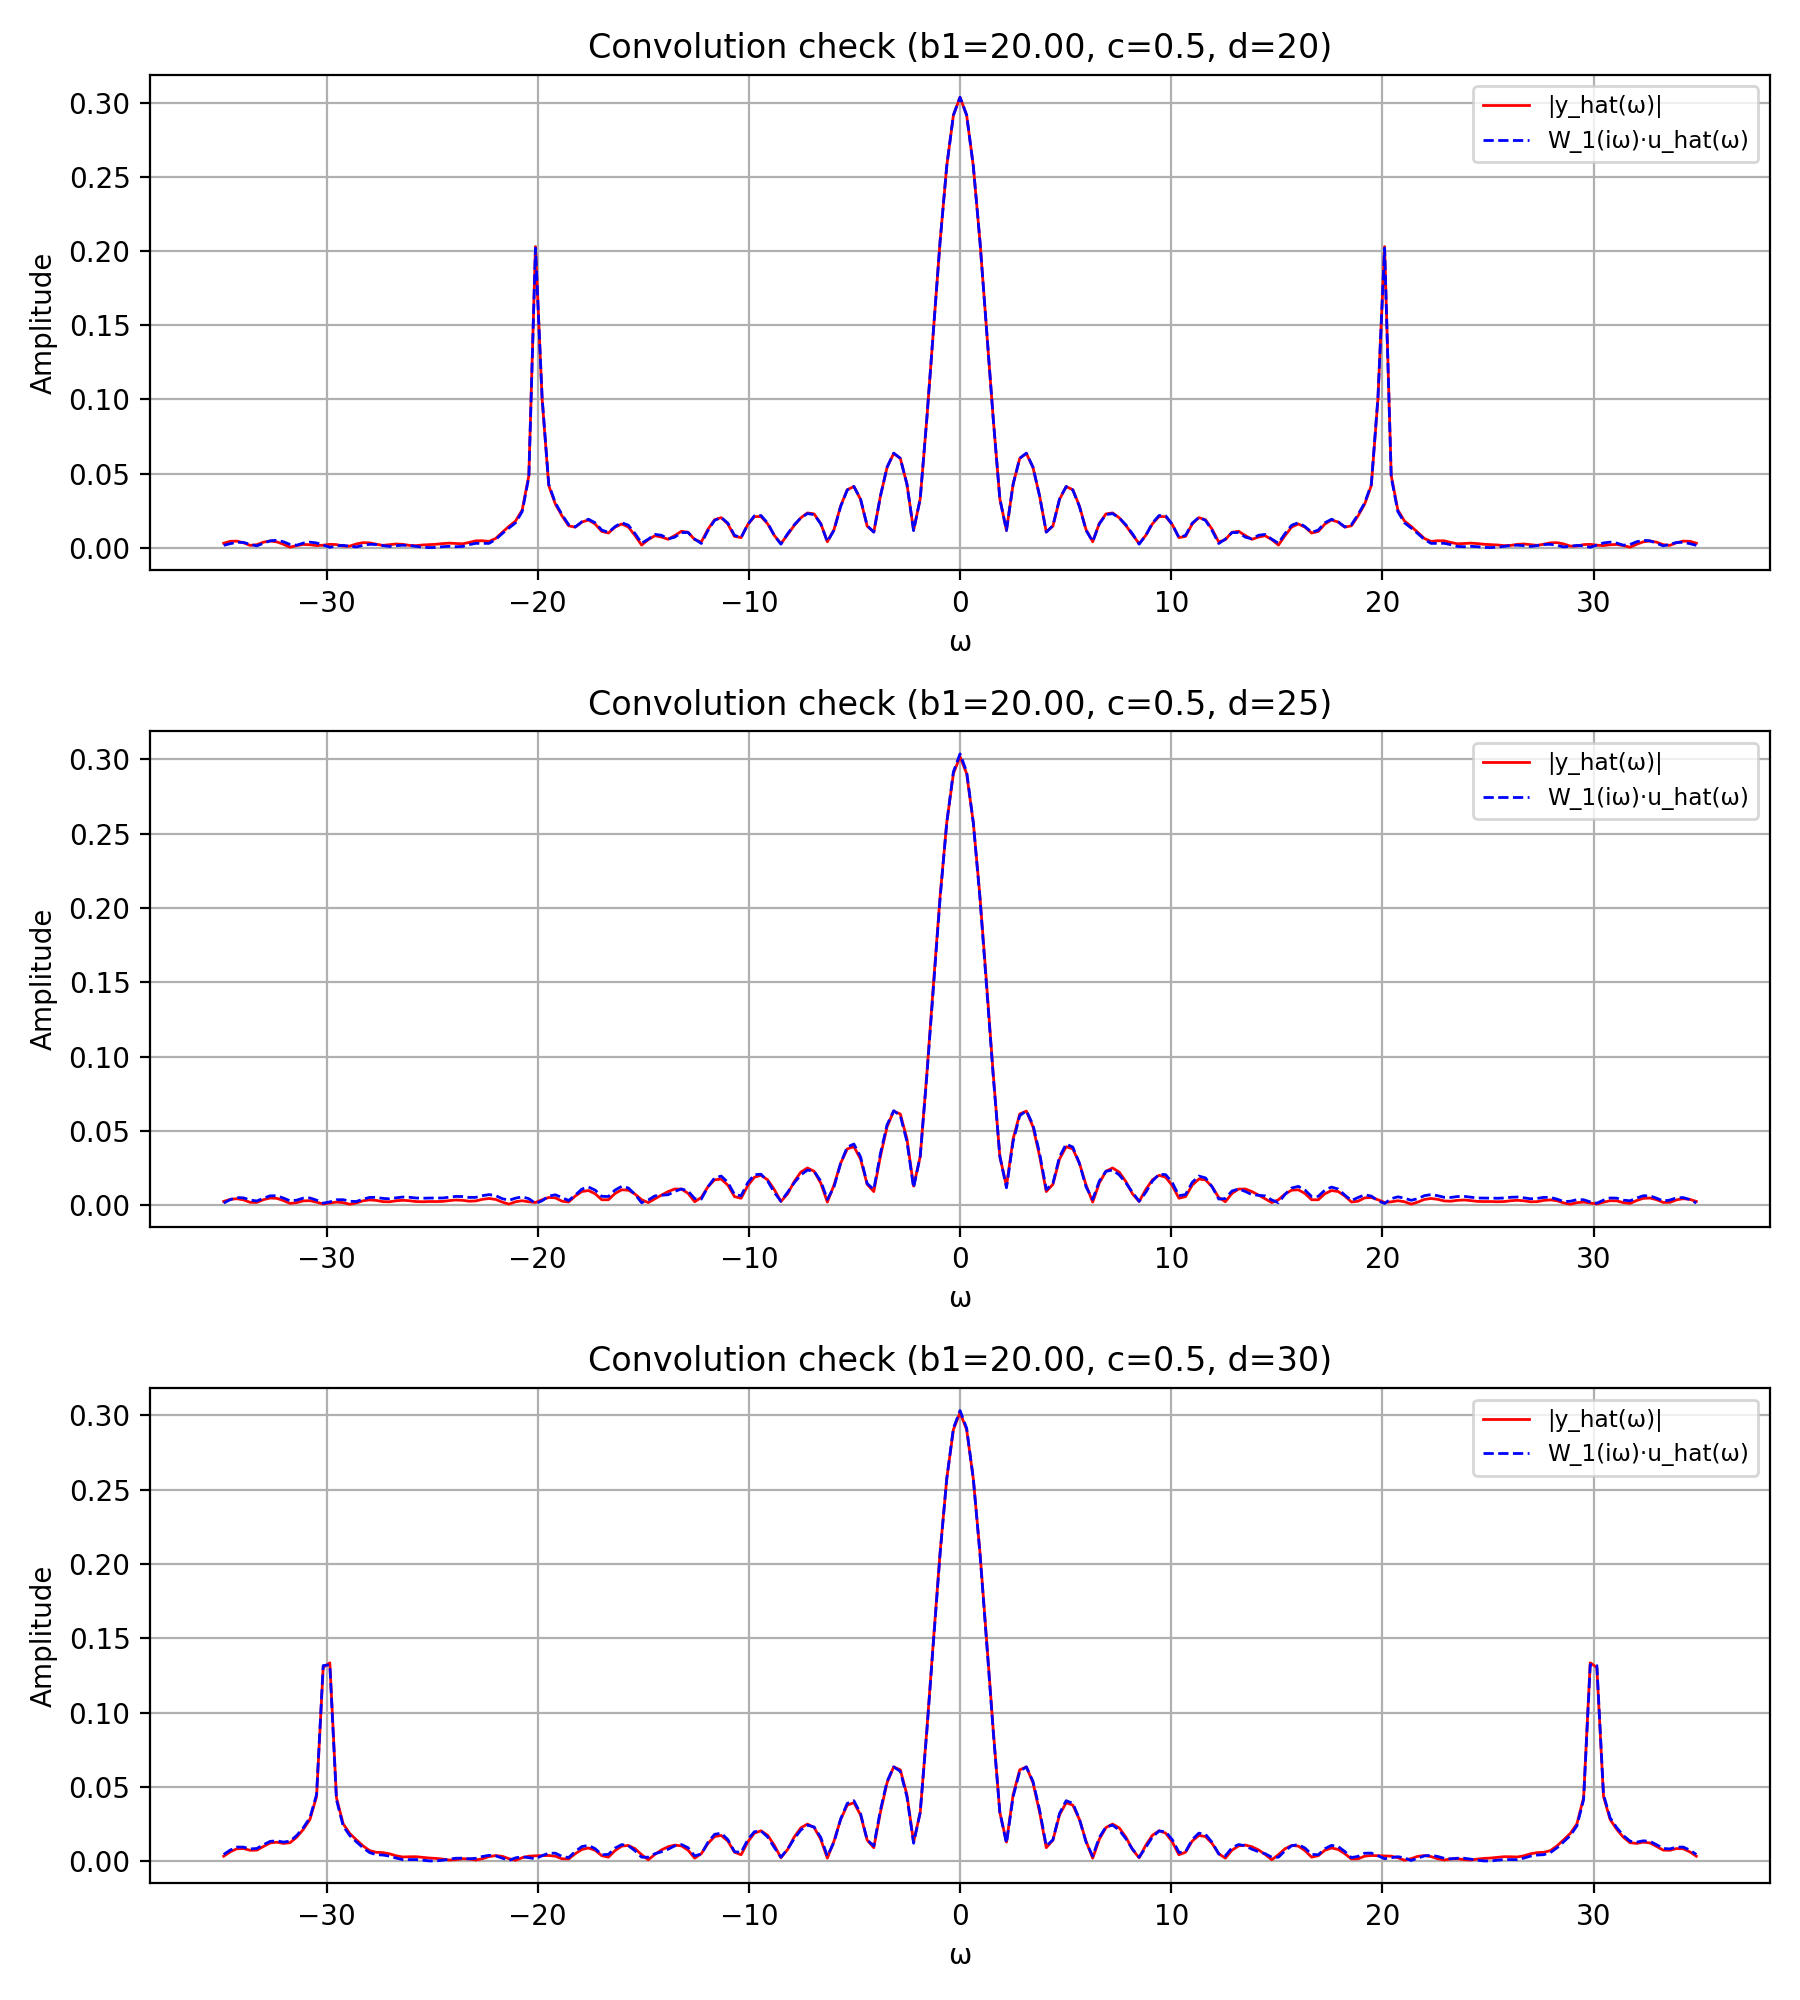
\includegraphics[width=1.0\linewidth]{fig/plots/Figure 44.png}
    \caption{Частотная область}
    \label{fig:44}
\end{figure}
\begin{figure}[H]
    \centering
    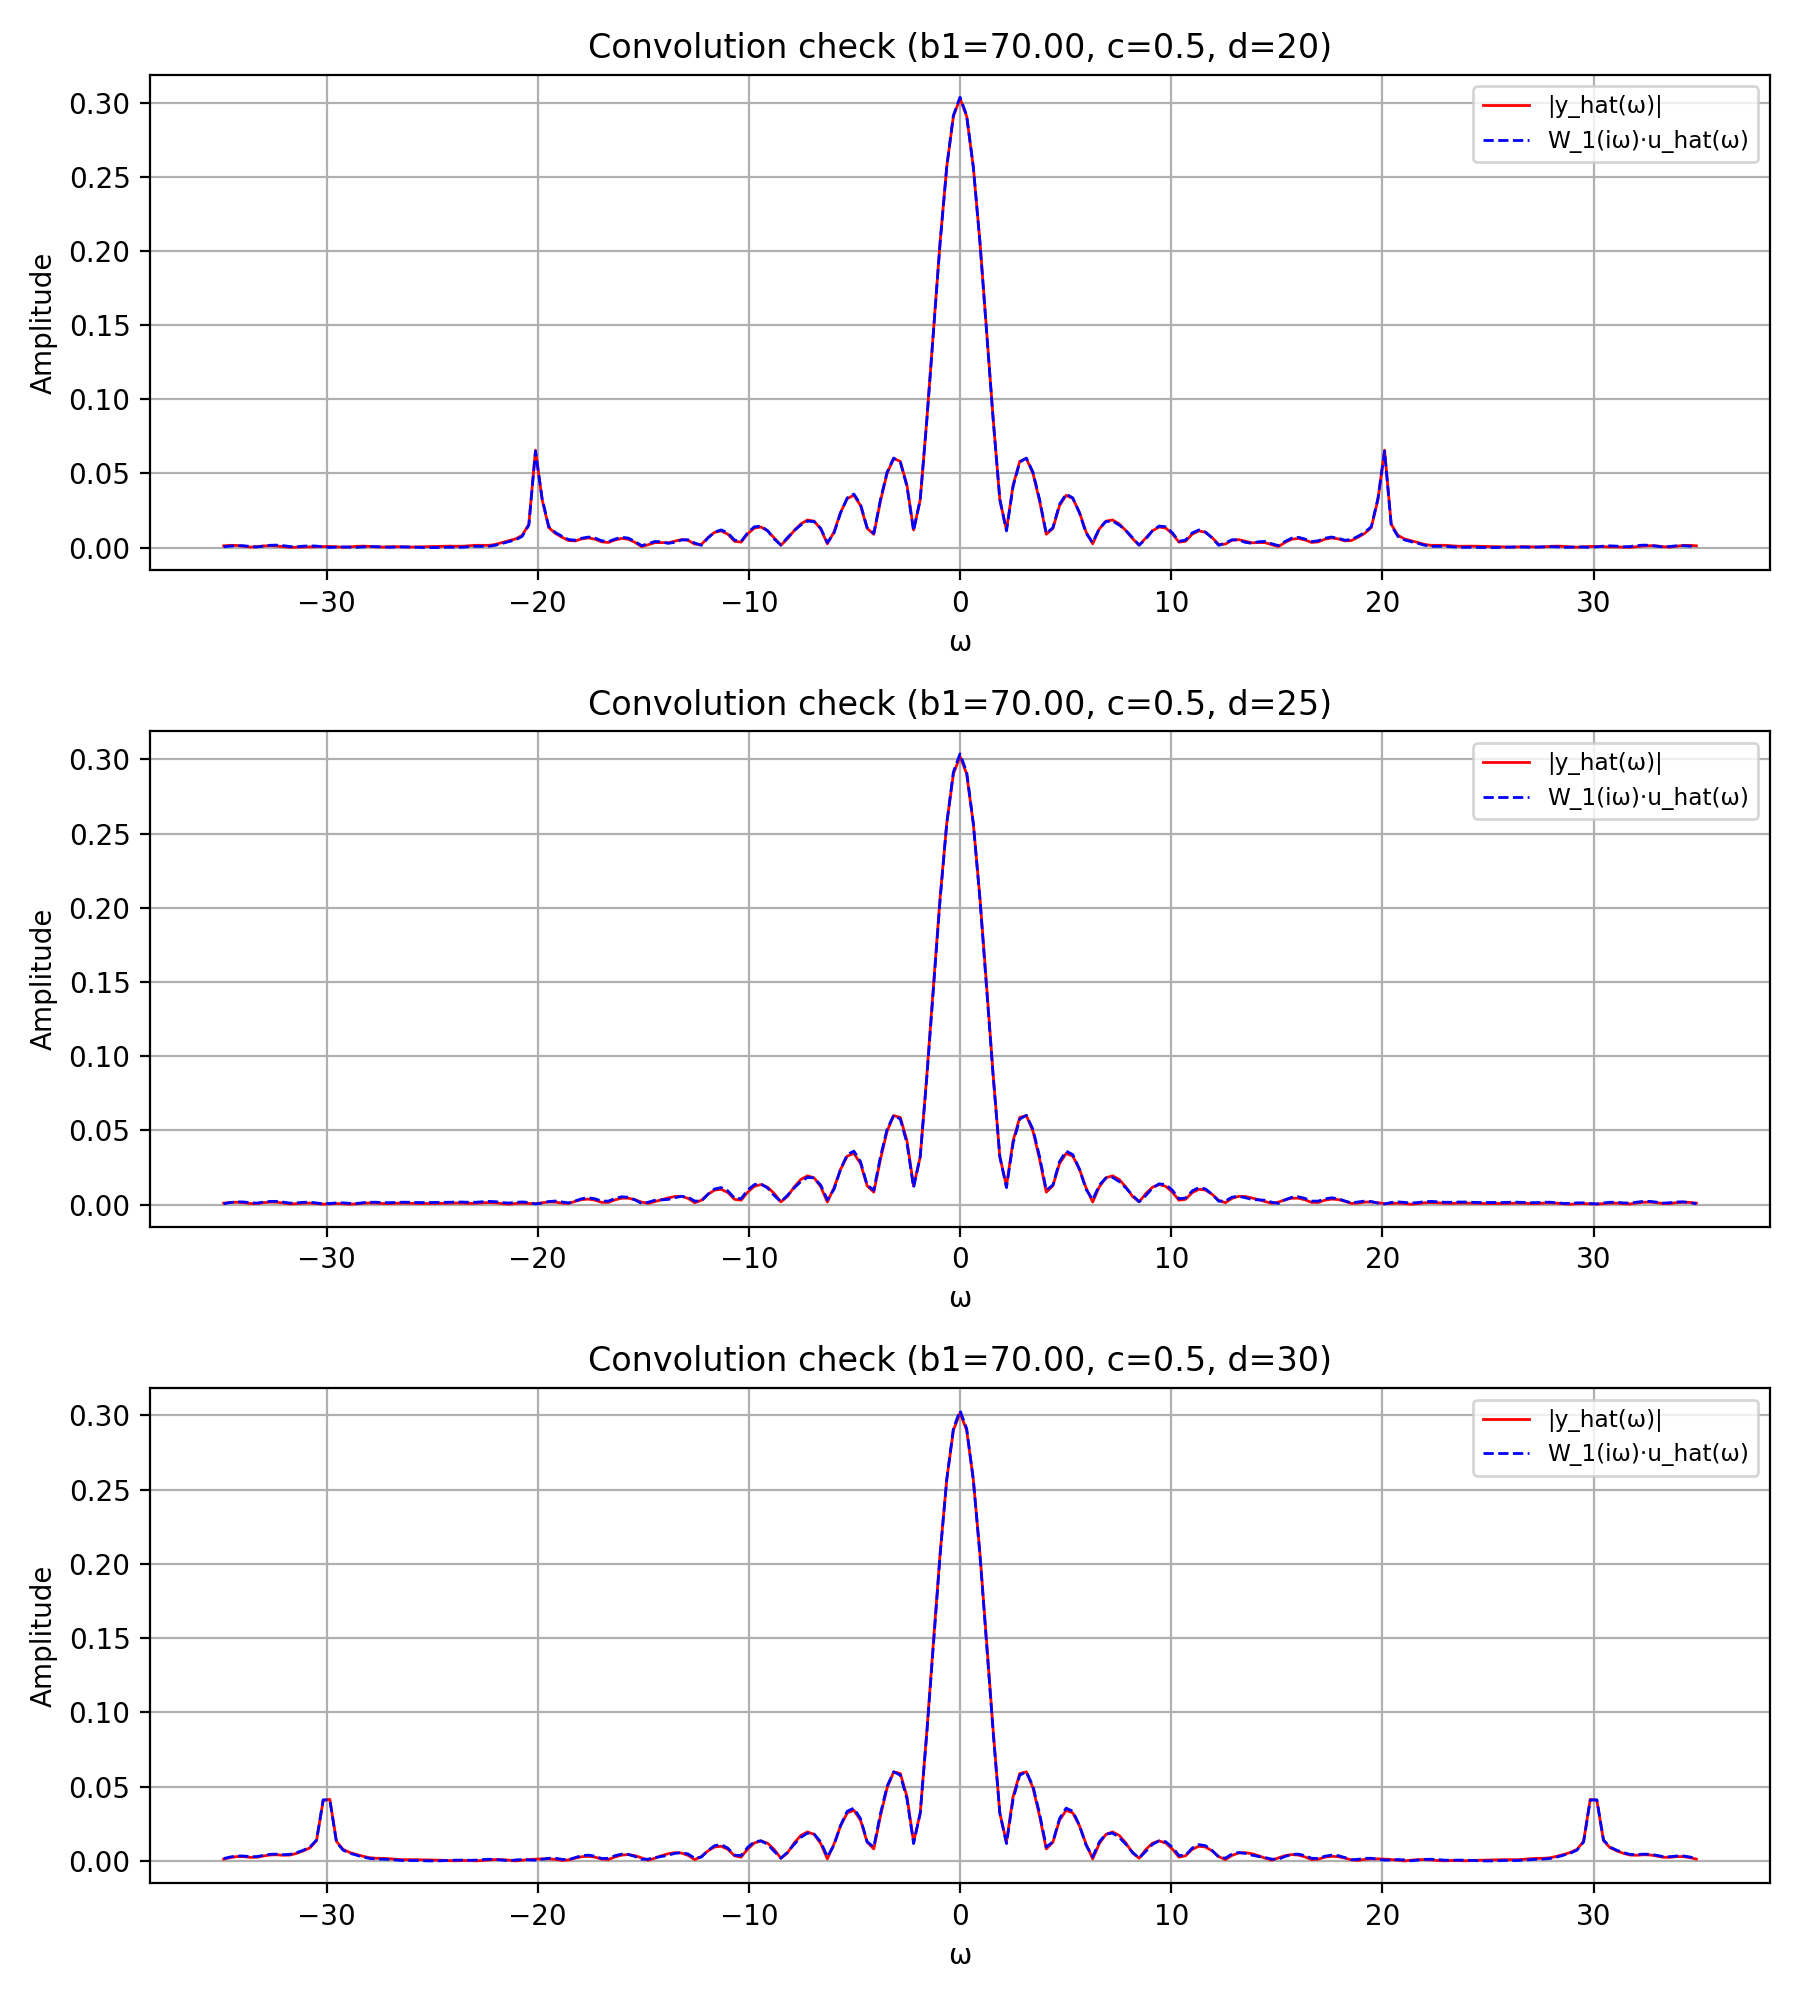
\includegraphics[width=1.0\linewidth]{fig/plots/Figure 45.png}
    \caption{Частотная область}
    \label{fig:45}
\end{figure}
\begin{figure}[H]
    \centering
    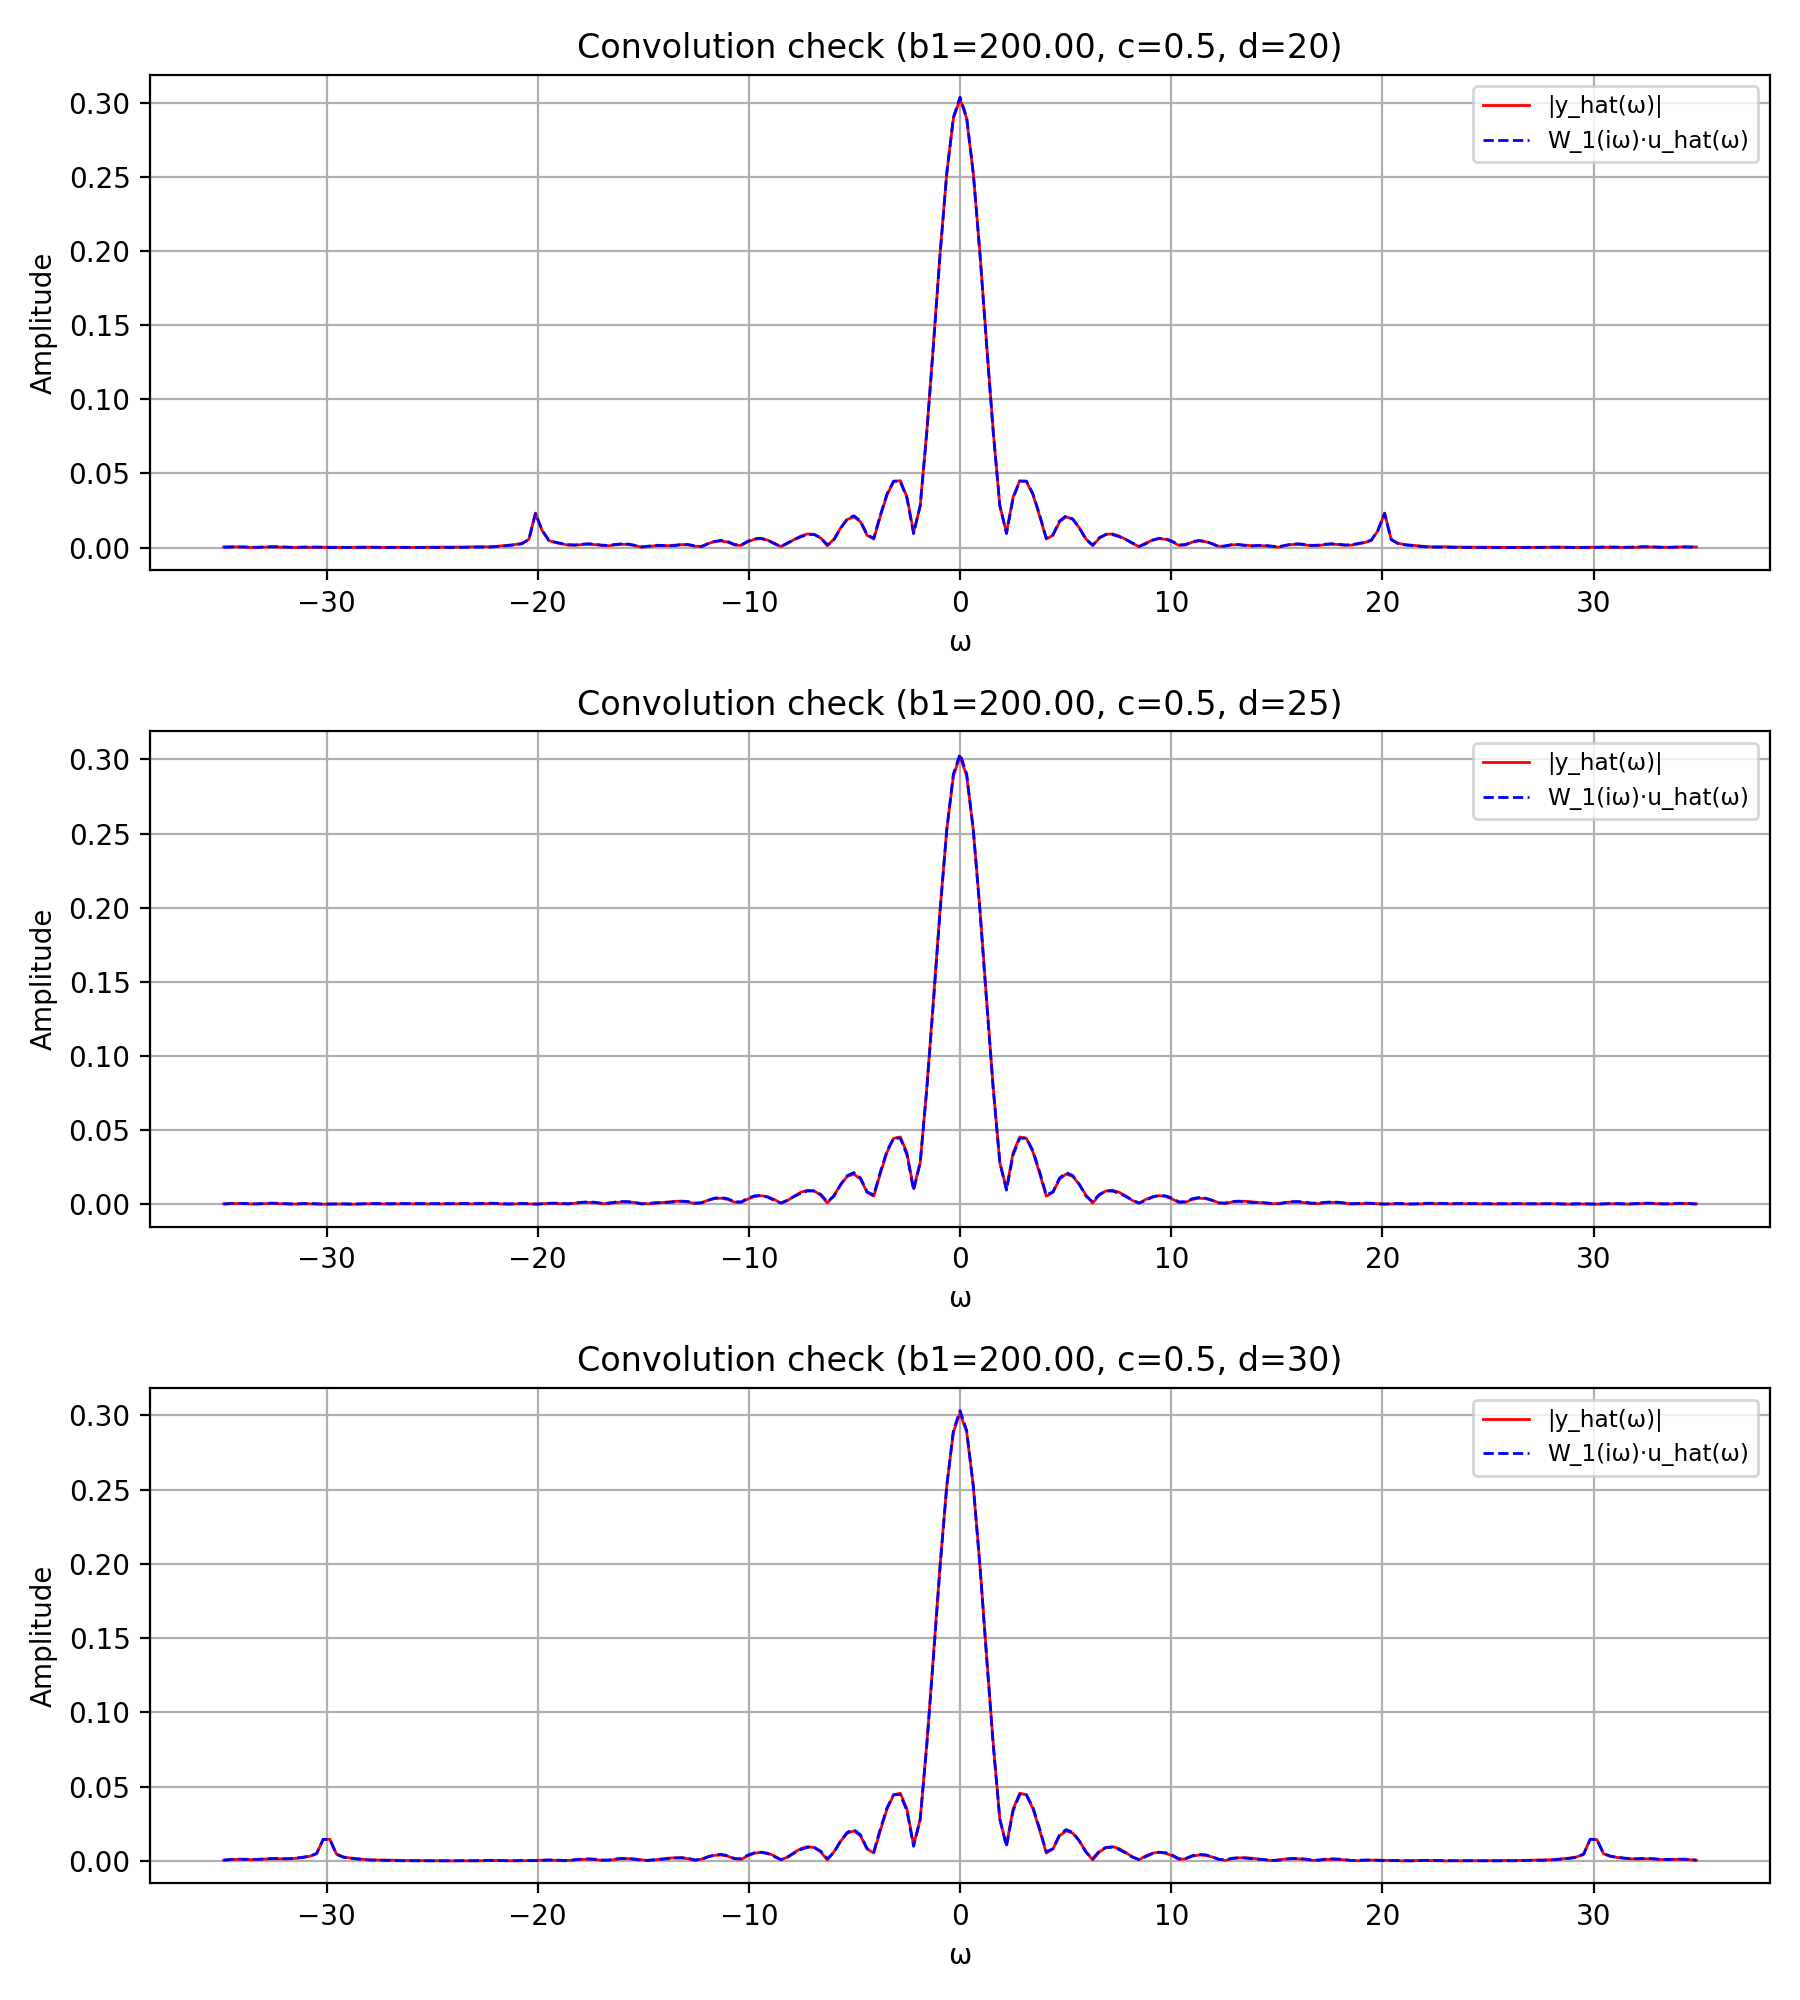
\includegraphics[width=1.0\linewidth]{fig/plots/Figure 46.png}
    \caption{Частотная область}
    \label{fig:46}
\end{figure}

\newpage
\section{Задание 2. Сглаживание биржевых данных}
Вообразим, что мы разрабатываем инвестиционное приложение, в котором должна присутствовать функция представления сглаженных графиков котировок акций.
\newline
При этом степень сглаживания должна зависеть от рассматриваемого нами временного периода.
\newline
Скачаем \href{fig:https://www.finam.ru/quote/moex/sber/export/}{отсюда} файл с данными о стоимости акций Сбербанка за достаточно продолжительный период. Загрузим данные в Python и применим к ним линейную фильтрацию с помощью фильтра первого порядка. Последовательно возьмём следующие значения постоянной времени $T$ : 1 день, 1 неделя, 1 месяц, 3 месяца, 1 год. Построим сравнительные графики исходного и фильтрованного сигналов, красиво оформим результат.
\newline
Возьём данные за период $10.06.2021-10.06.2025$ и будем анализировать цену закрытия (см. рис. \ref{fig:47}).
\newline
\textbf{Выводы}
\newline
Линейная фильтрация может использована не только для обработки сигналов, но и быть так же полезна при анализе финансовых инструментов. Однако, на практике стоит применять более сложные фильтры, так как можно заметить, что данный вариант хуже справляется со сглаживанием там, где происходят резкие изменения в цене. В нашем рассмотренном варианте больше всего подходят случае $T$: 1 день и 1 неделя, при большем $T$ сглаживание начинает съедать слишком много информации о цене.
\newline
\textbf{Общий вывод}\newline
Линейная фильтрация - эффективный инструмент для обработки сигналов и работы со сглаживанием графиков. Преимущество динамической фильтрации заключается в её вохможности работать с сигналом непосредственно по мере его получения, что делает её востребованной в реальных практических задачах.

\begin{figure}[H]
    \centering
    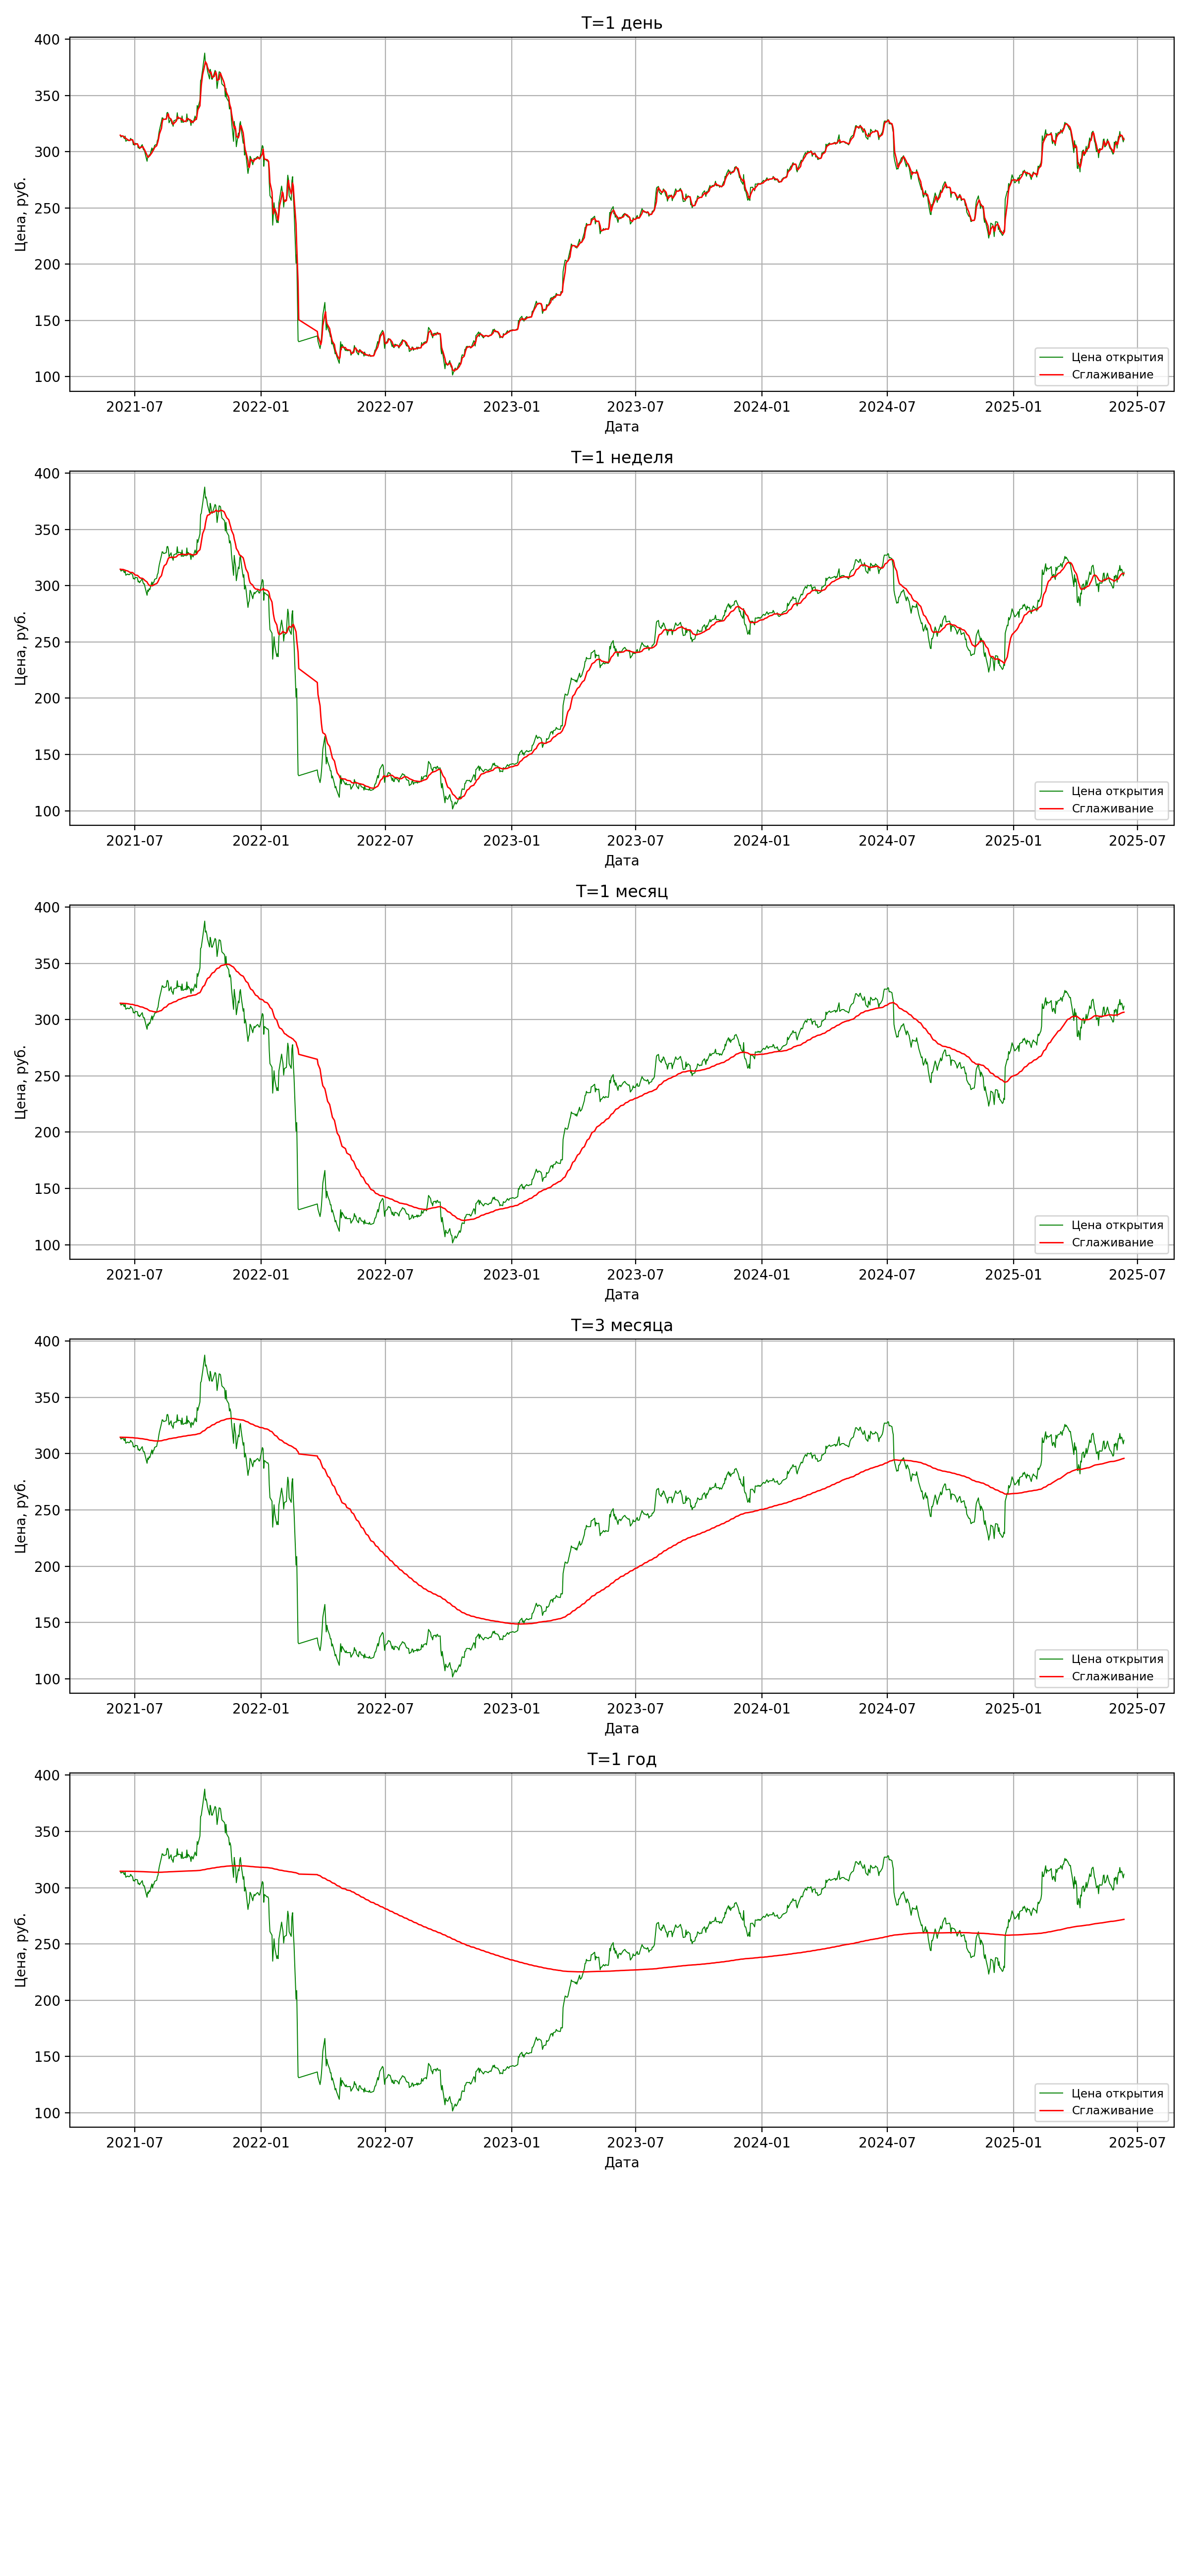
\includegraphics[width=0.83\linewidth]{fig/plots/Figure 47.png}
    \caption{Цена закрытия}
    \label{fig:47}
\end{figure}

\newpage
\section{Приложение}
\begin{code}
	\inputminted[breaklines=true, xleftmargin=1em, linenos, frame=single, framesep=10pt, fontsize=\tiny, firstline=1, lastline=720]{python}{/home/ns/Desktop/ITMO-courses/Fourier_Methods/Lab4/tex/FM_Lab4/listings/listing_lab4.py}
	\caption{Листинг}
\end{code}